\input{preamble}

% OK, start here.
%
\usepackage{fontspec}
\let\hyperwhite\relax
\let\hyperred\relax
\newcommand{\hyperwhite}{\hypersetup{citecolor=white,filecolor=white,linkcolor=white,urlcolor=white}}
\newcommand{\hyperred}{%
\hypersetup{%
    citecolor=TitlingRed,%
    filecolor=TitlingRed,%
    linkcolor=TitlingRed,%
     urlcolor=TitlingRed%
}}
\let\ChapterRef\relax
\newcommand{\ChapterRef}[2]{#1}
\setcounter{tocdepth}{2}
%▓▓▓▓▓▓▓▓▓▓▓▓▓▓▓▓▓▓▓▓▓▓▓▓▓▓▓▓▓▓▓▓▓
%▓▓ ╔╦╗╦╔╦╗╦  ╔═╗  ╔═╗╔═╗╔╗╔╔╦╗ ▓▓
%▓▓  ║ ║ ║ ║  ║╣   ╠╣ ║ ║║║║ ║  ▓▓
%▓▓  ╩ ╩ ╩ ╩═╝╚═╝  ╚  ╚═╝╝╚╝ ╩  ▓▓
%▓▓▓▓▓▓▓▓▓▓▓▓▓▓▓▓▓▓▓▓▓▓▓▓▓▓▓▓▓▓▓▓▓
%\usepackage{titlesec}
%▓▓▓▓▓▓▓▓▓▓▓▓▓▓▓▓▓▓▓▓▓▓▓▓▓▓▓▓▓▓▓▓▓▓▓▓▓▓▓▓▓▓▓▓▓▓▓▓▓▓▓▓▓▓▓
%▓▓ ╔╦╗╔═╗╔╗ ╦  ╔═╗  ╔═╗╔═╗  ╔═╗╔═╗╔╗╔╔╦╗╔═╗╔╗╔╔╦╗╔═╗ ▓▓
%▓▓  ║ ╠═╣╠╩╗║  ║╣   ║ ║╠╣   ║  ║ ║║║║ ║ ║╣ ║║║ ║ ╚═╗ ▓▓
%▓▓  ╩ ╩ ╩╚═╝╩═╝╚═╝  ╚═╝╚    ╚═╝╚═╝╝╚╝ ╩ ╚═╝╝╚╝ ╩ ╚═╝ ▓▓
%▓▓▓▓▓▓▓▓▓▓▓▓▓▓▓▓▓▓▓▓▓▓▓▓▓▓▓▓▓▓▓▓▓▓▓▓▓▓▓▓▓▓▓▓▓▓▓▓▓▓▓▓▓▓▓
\newcommand{\ChapterTableOfContents}{%
    \begingroup
    \addfontfeature{Numbers={Lining,Monospaced}}
    \hypersetup{hidelinks}\tableofcontents%
    \endgroup
}%

\makeatletter
\newcommand \DotFill {\leavevmode \cleaders \hb@xt@ .33em{\hss .\hss }\hfill \kern \z@}
\makeatother

\definecolor{ToCGrey}{rgb}{0.4,0.4,0.4}
\definecolor{mainColor}{rgb}{0.82745098,0.18431373,0.18431373}
\usepackage{titletoc}
\titlecontents{part}
[0.0em]
{\addvspace{1pc}\color{TitlingRed}\large\bfseries\text{Part }}
{\bfseries\textcolor{TitlingRed}{\contentslabel{0.0em}}\hspace*{1.35em}}
{}
{\textcolor{TitlingRed}{{\hfill\bfseries\contentspage\nobreak}}}
[]
\titlecontents{section}
[0.0em]
{\addvspace{1pc}}
{\color{black}\bfseries\textcolor{TitlingRed}{\contentslabel{0.0em}}\hspace*{1.35em}}
{}
{\textcolor{black}{\textbf{\DotFill}{\bfseries\contentspage\nobreak}}}
[]
\titlecontents{subsection}
[0.0em]
{}
{\hspace*{1.35em}\color{ToCGrey}{\contentslabel{0.0em}}\hspace*{2.1em}}
{}
{{\textcolor{ToCGrey}\DotFill}\textcolor{ToCGrey}{\contentspage}\nobreak}
[]
\usepackage{marginnote}
\renewcommand*{\marginfont}{\normalfont}
\usepackage{inconsolata}
\setmonofont{inconsolata}%
\let\ChapterRef\relax
\newcommand{\ChapterRef}[2]{#1}
\AtBeginEnvironment{subappendices}{%%
    \section*{\huge Appendices}%
}%

\begin{document}

\title{Constructions With Sets}

\maketitle

\phantomsection
\label{section-phantom}

This chapter develops some material relating to constructions with sets with an eye towards its categorical and higher-categorical counterparts to be introduced later in this work. In particular, it contains:
\begin{enumerate}
    \item Explicit descriptions of the major types of co/limits in $\Sets$, including in particular explicit descriptions of pushouts and coequalisers (see \cref{pushouts-of-sets,unwinding-pushouts-of-sets,coequalisers-of-sets,unwinding-coequalisers-of-sets}).
    \item A discussion of powersets as decategorifications of categories of presheaves (\cref{characteristic-functions-as-decategorifications-of-presheaves,powersets-as-decategorifications-of-co-presheaf-categories}), including a $(-1)$-categorical analogue of un/straightening, described in \cref{properties-of-powersets-as-sets-of-functions-relations-powersets-as-sets-of-functions-1,properties-of-powersets-as-sets-of-functions-relations-powersets-as-sets-of-functions-2} of \cref{properties-of-powersets-as-sets-of-functions-relations} and \cref{powersets-as-sets-of-functions-and-un-straightening}.
    \item A lengthy discussion of the adjoint triple%
        \[
            f_{*}\dashv f^{-1}\dashv f_{!}%
            \colon%
            \mathcal{P}(A)%
            \rightleftrightarrows%
            \mathcal{P}(B)%
        \]%
        of functors (morphisms of posets) between $\mathcal{P}(A)$ and $\mathcal{P}(B)$ induced by a map of sets $f\colon A\to B$, along with a discussion of the properties of $f_{*}$, $f^{-1}$, and $f_{!}$.%

        In line with the categorical viewpoint developed here, this adjoint triple may be described in terms of Kan extensions, and, as it turns out, it also shows up in some definitions and results in point-set topology, such as in e.g.\ notions of continuity for functions (\ChapterRef{\ChapterTopologicalSpaces, \cref{topological-spaces:section-continuous-maps}}{\cref{section-continuous-maps}}).
\end{enumerate}

\ChapterTableOfContents

\section{Limits of Sets}\label{section-limits-of-sets}
\subsection{The Terminal Set}\label{subsection-the-terminal-set}
\begin{definition}{The Terminal Set}{the-terminal-set}%
    The \index[set-theory]{terminal set}\textbf{terminal set} is the pair \index[notation]{pt@$\pt$}$(\pt,\{!_{A}\}_{A\in\Obj(\Sets)})$ consisting of:
    \begin{itemize}
        \item\SloganFont{The Limit. }The punctual set $\pt\defeq\{\point\}$.
        \item\SloganFont{The Cone. }The collection of maps
            \[
                \{%
                    !_{A}%
                    \colon%
                    A%
                    \to%
                    \pt%
                \}_{A\in\Obj(\Sets)}%
            \]%
            defined by
            \[
                !_{A}(a)%
                \defeq%
                \point%
            \]%
            for each $a\in A$ and each $A\in\Obj(\Sets)$.
    \end{itemize}
\end{definition}
\begin{Proof}{Proof of \cref{the-terminal-set}}%
    We claim that $\pt$ is the terminal object of $\Sets$. Indeed, suppose we have a diagram of the form
    \[
        \begin{tikzcd}[row sep={3.0*\the\DL,between origins}, column sep={4.0*\the\DL,between origins}, background color=backgroundColor, ampersand replacement=\&]
            A
            \&
            \pt
        \end{tikzcd}
    \]%
    in $\Sets$. Then there exists a unique map $\phi\colon A\to\pt$ making the diagram
    \[
        \begin{tikzcd}[row sep={3.0*\the\DL,between origins}, column sep={4.0*\the\DL,between origins}, background color=backgroundColor, ampersand replacement=\&]
            A
            \arrow[r,"\phi"{pos=0.425},"\exists!"'{pos=0.425}, dashed]
            \&
            \pt
        \end{tikzcd}
    \]%
    commute, namely $!_{A}$.
\end{Proof}
\subsection{Products of Families of Sets}\label{subsection-products-of-families-of-sets}
Let $\{A_{i}\}_{i\in I}$ be a family of sets.%
\begin{definition}{The Product of a Family of Sets}{the-product-of-a-family-of-sets}%
    The \index[set-theory]{product of a family of sets}\textbf{product}%
    %--- Begin Footnote ---%
    \footnote{%
        \SloganFont{Further Terminology: }Also called the \index[set-theory]{Cartesian product}\textbf{Cartesian product of $\{A_{i}\}_{i\in I}$}.
    } %
    %---  End Footnote  ---%
    \textbf{of $\{A_{i}\}_{i\in I}$} is the pair \index[notation]{prodiiniai@$\prod_{i\in I}A_{i}$}$(\prod_{i\in I}A_{i},\{\pr_{i}\}_{i\in I})$ consisting of:
    \begin{itemize}
        \item\SloganFont{The Limit. }The set $\prod_{i\in I}A_{i}$ defined by%
            %--- Begin Footnote ---%
            \footnote{%
                Less formally, $\prod_{i\in I}A_{i}$ is the set whose elements are $I$-indexed collections $(a_{i})_{i\in I}$ with $a_{i}\in A_{i}$ for each $i\in I$. The projection maps
                \[
                    \{%
                        \pr_{i}
                        \colon%
                        \prod_{i\in I}A_{i}%
                        \to%
                        A_{i}%
                    \}_{i\in I}%
                \]%
                are then given by
                \[
                    \pr_{i}((a_{j})_{j\in I})%
                    \defeq%
                    a_{i}%
                \]%
                for each $(a_{j})_{j\in I}\in\prod_{i\in I}A_{i}$ and each $i\in I$.
                \par\vspace*{-1.75\baselineskip}
            }%
            %---  End Footnote  ---%
            \[
                \prod_{i\in I}A_{i}
                \defeq
                \{%
                    f\in\Sets(I,\bigcup_{i\in I}A_{i})%
                    \ \middle|\ %
                    \parbox{0.225\textwidth}{%
                        for each $i\in I$, we have $f(i)\in A_{i}$%
                    }%
                \}.%
            \]%
        \item\SloganFont{The Cone. }The collection
            \[
                \{%
                    \pr_{i}
                    \colon%
                    \prod_{i\in I}A_{i}%
                    \to%
                    A_{i}%
                \}_{i\in I}%
            \]%
            of maps given by%
            \[
                \pr_{i}(f)%
                \defeq%
                f(i)%
            \]%
            for each $f\in\prod_{i\in I}A_{i}$ and each $i\in I$.
    \end{itemize}
\end{definition}
\begin{Proof}{Proof of \cref{the-product-of-a-family-of-sets}}%
    We claim that $\prod_{i\in I}A_{i}$ is the categorical product of $\{A_{i}\}_{i\in I}$ in $\Sets$. Indeed, suppose we have, for each $i\in I$, a diagram of the form
    \[
        \begin{tikzcd}[row sep={5.0*\the\DL,between origins}, column sep={5.0*\the\DL,between origins}, background color=backgroundColor, ampersand replacement=\&]
            P
            \arrow[rd,"p_{i}"]
            \&
            \\
            {\displaystyle\prod_{i\in I}A_{i}}
            \arrow[r,"\pr_{i}"']
            \&
            A_{i}
        \end{tikzcd}
    \]%
    in $\Sets$. Then there exists a unique map $\phi\colon P\to\prod_{i\in I}A_{i}$ making the diagram
    \[
        \begin{tikzcd}[row sep={5.0*\the\DL,between origins}, column sep={5.0*\the\DL,between origins}, background color=backgroundColor, ampersand replacement=\&]
            P
            \arrow[rd,"p_{i}"]
            \arrow[d,"\phi"',"\exists!",dashed]
            \&
            \\
            {\displaystyle\prod_{i\in I}A_{i}}
            \arrow[r,"\pr_{i}"']
            \&
            A_{i}
        \end{tikzcd}
    \]%
    commute, being uniquely determined by the condition $\pr_{i}\circ\phi=p_{i}$ for each $i\in I$ via
    \[
        \phi(x)%
        =%
        (p_{i}(x))_{i\in I}
    \]%
    for each $x\in P$.
\end{Proof}
\begin{proposition}{Properties of Products of Families of Sets}{properties-of-products-of-families-of-sets}%
    Let $\{A_{i}\}_{i\in I}$ be a family of sets.%
    \begin{enumerate}
        \item\label{properties-of-products-of-families-of-sets-functoriality}\SloganFont{Functoriality. }The assignment $\{A_{i}\}_{i\in I}\mapsto\prod_{i\in I}A_{i}$ defines a functor
            \[
                \prod_{i\in I}%
                \colon%
                \Fun(I_{\disc},\Sets)%
                \to%
                \Sets%
            \]%
            where
            \begin{itemize}
                \item\SloganFont{Action on Objects. }For each $(A_{i})_{i\in I}\in\Obj(\Fun(I_{\disc},\Sets))$, we have
                    \[
                        \left[\prod_{i\in I}\right]((A_{i})_{i\in I})%
                        \defeq%
                        \prod_{i\in I}A_{i}%
                    \]%
                \item\SloganFont{Action on Morphisms. }For each $(A_{i})_{i\in I},(B_{i})_{i\in I}\in\Obj(\Fun(I_{\disc},\Sets))$, the action on $\Hom$-sets
                    \[
                        (\prod_{i\in I})_{(A_{i})_{i\in I},(B_{i})_{i\in I}}
                        \colon
                        \Nat((A_{i})_{i\in I},(B_{i})_{i\in I})%
                        \to%
                        \Sets(\prod_{i\in I}A_{i},\prod_{i\in I}B_{i})%
                    \]%
                    of $\prod_{i\in I}$ at $((A_{i})_{i\in I},(B_{i})_{i\in I})$ is defined by sending a map
                    \[
                        \{%
                            f_{i}%
                            \colon%
                            A_{i}%
                            \to%
                            B_{i}
                        \}_{i\in I}%
                        %
                    \]%
                    in $\Nat((A_{i})_{i\in I},(B_{i})_{i\in I})$ to the map of sets
                    \[
                        \prod_{i\in I}f_{i}%
                        \colon
                        \prod_{i\in I}A_{i}%
                        \to%
                        \prod_{i\in I}B_{i}%
                    \]%
                    defined by
                    \[
                        \left[\prod_{i\in I}f_{i}\right]((a_{i})_{i\in I})
                        \defeq%
                        (f_{i}(a_{i}))_{i\in I}
                    \]%
                    for each $(a_{i})_{i\in I}\in\prod_{i\in I}A_{i}$.
            \end{itemize}
        %\item\label{properties-of-products-of-families-of-sets-}\SloganFont{. }
    \end{enumerate}
\end{proposition}
\begin{Proof}{Proof of \cref{properties-of-products-of-families-of-sets}}%
    \FirstProofBox{\cref{properties-of-products-of-families-of-sets-functoriality}: Functoriality}%
    This follows from \ChapterRef{\ChapterLimitsAndColimits, \cref{limits-and-colimits:properties-of-co-limits-functoriality} of \cref{limits-and-colimits:properties-of-co-limits}}{\cref{properties-of-co-limits-functoriality} of \cref{properties-of-co-limits}}.
\end{Proof}
\subsection{Binary Products of Sets}\label{subsection-binary-products-of-sets}
Let $A$ and $B$ be sets.%
\begin{definition}{Products of Sets}{products-of-sets}%
    The \index[set-theory]{product of sets}\textbf{product}%
    %--- Begin Footnote ---%
    \footnote{%
        \SloganFont{Further Terminology: }Also called the \index[set-theory]{Cartesian product}\textbf{Cartesian product of $A$ and $B$} or the \textbf{binary Cartesian product of $A$ and $B$}, for emphasis.

        This can also be thought of as the \textbf{$(\E_{-1},\E_{-1})$-tensor product of $A$ and $B$}.
    } %
    %---  End Footnote  ---%
    \textbf{of $A$ and $B$} is the pair \index[notation]{AtimesB@$A\times B$}$(A\times B,\{\pr_{1},\pr_{2}\})$ consisting of:
    \begin{itemize}
        \item\SloganFont{The Limit. }The set $A\times B$ defined by%
            %--- Begin Footnote ---%
            \footnote{%
                In other words, $A\times B$ is the set whose elements are ordered pairs $(a,b)$ with $a\in A$ and $b\in B$ as in \cref{ordered-pairs}
                \par\vspace*{-1.75\baselineskip}
            }%
            %---  End Footnote  ---%
            \begin{align*}
                A\times B &\defeq \prod_{z\in\{A,B\}}z\\
                          &\defeq \{%
                                      f\in\Sets(\{0,1\},A\cup B)%
                                      \ \middle|\ %
                                      \text{%
                                          we have $f(0)\in A$ and $f(1)\in B$%
                                      }%
                                  \}\\%
                          &\cong \{\{\{a\},\{a,b\}\}\in\mathcal{P}(\mathcal{P}(A\cup B))\ \middle|\ \text{we have $a\in A$ and $b\in B$}\}.%
            \end{align*}
        \item\SloganFont{The Cone. }The maps
            \begin{align*}
                \pr_{1} &\colon A\times B\to A,\\
                \pr_{2} &\colon A\times B\to B
            \end{align*}
            defined by
            \begin{align*}
                \pr_{1}(a,b) &\defeq a,\\
                \pr_{2}(a,b) &\defeq b
            \end{align*}
            for each $(a,b)\in A\times B$.
    \end{itemize}
\end{definition}
\begin{Proof}{Proof of \cref{products-of-sets}}%
    We claim that $A\times B$ is the categorical product of $A$ and $B$ in $\Sets$. Indeed, suppose we have a diagram of the form
    \[
        \begin{tikzcd}[row sep={4.0*\the\DL,between origins}, column sep={5.0*\the\DL,between origins}, background color=backgroundColor, ampersand replacement=\&]
            \&
            P
            \arrow[ld,"p_{1}"',bend right = 20]
            \arrow[rd,"p_{2}", bend left  = 20]
            \&
            \\
            A
            \&
            A\times B
            \arrow[l,"\pr_{1}"]
            \arrow[r,"\pr_{2}"']
            \&
            B
        \end{tikzcd}
    \]%
    in $\Sets$. Then there exists a unique map $\phi\colon P\to A\times B$ making the diagram
    \[
        \begin{tikzcd}[row sep={4.0*\the\DL,between origins}, column sep={5.0*\the\DL,between origins}, background color=backgroundColor, ampersand replacement=\&]
            \&
            P
            \arrow[ld,"p_{1}"',bend right = 20]
            \arrow[rd,"p_{2}", bend left  = 20]
            \arrow[d,"\phi"'{pos=0.425},"\exists!"{pos=0.425}, dashed]
            \&
            \\
            A
            \&
            A\times B
            \arrow[l,"\pr_{1}"]
            \arrow[r,"\pr_{2}"']
            \&
            B
        \end{tikzcd}
    \]%
    commute, being uniquely determined by the conditions
    \begin{align*}
        \pr_{1}\circ\phi &= p_{1},\\
        \pr_{2}\circ\phi &= p_{2}
    \end{align*}
    via
    \[
        \phi(x)%
        =%
        (p_{1}(x),p_{2}(x))%
    \]%
    for each $x\in P$.
\end{Proof}
\begin{proposition}{Properties of Products of Sets}{properties-of-products-of-sets}%
    Let $A$, $B$, $C$, and $X$ be sets.
    \begin{enumerate}
        \item\label{properties-of-products-of-sets-functoriality}\SloganFont{Functoriality. }The assignments $A,B,(A,B)\mapsto A\times B$ define functors
            \begin{gather*}
                \begin{aligned}
                    A\times-    &\colon            \Sets \to \Sets,\\
                    -\times B   &\colon \Sets            \to \Sets,
                \end{aligned}\\
                -_{1}\times-_{2} \colon \Sets\times\Sets \to \Sets,
            \end{gather*}
            where $-_{1}\times-_{2}$ is the functor where
            \begin{itemize}
                \item\SloganFont{Action on Objects. }For each $(A,B)\in\Obj(\Sets\times\Sets)$, we have
                    \[
                        [-_{1}\times-_{2}](A,B)%
                        \defeq
                        A\times B.%
                    \]%
                \item\SloganFont{Action on Morphisms. }For each $(A,B),(X,Y)\in\Obj(\Sets)$, the action on $\Hom$-sets
                    \[
                        \times_{(A,B),(X,Y)}
                        \colon
                        \Sets(A,X)\times\Sets(B,Y)%
                        \to%
                        \Sets(A\times B,X\times Y)%
                    \]%
                    of $\times$ at $((A,B),(X,Y))$ is defined by sending $(f,g)$ to the function
                    \[
                        f\times g%
                        \colon%
                        A\times B%
                        \to%
                        X\times Y%
                    \]%
                    defined by
                    \[
                        [f\times g](a,b)%
                        \defeq%
                        (f(a),g(b))
                    \]%
                    for each $(a,b)\in A\times B$.
            \end{itemize}
            and where $A\times-$ and $-\times B$ are the partial functors of $-_{1}\times-_{2}$ at $A,B\in\Obj(\Sets)$.
        \item\label{properties-of-products-of-sets-adjointness}\SloganFont{Adjointness. }We have adjunctions
            \begin{webcompile}
                \begin{gathered}
                    \AdjunctionShort#A\times -#{\Hom_{\Sets}(A,-)}#\Sets#\Sets,#\\
                    \AdjunctionShort#-\times B#{\Hom_{\Sets}(B,-)}#\Sets#\Sets,#
                \end{gathered}
            \end{webcompile}%
            witnessed by bijections
            \begin{align*}
                \Hom_{\Sets}(A\times B,C) &\cong \Hom_{\Sets}(A,\Hom_{\Sets}(B,C)),\\
                \Hom_{\Sets}(A\times B,C) &\cong \Hom_{\Sets}(B,\Hom_{\Sets}(A,C)),
            \end{align*}
            natural in $A,B,C\in\Obj(\Sets)$.
        \item\label{properties-of-products-of-sets-associativity}\SloganFont{Associativity. }We have an isomorphism of sets%
            \[
                (A\times B)\times C
                \cong
                A\times(B\times C),
            \]%
            natural in $A,B,C\in\Obj(\Sets)$.
        \item\label{properties-of-products-of-sets-unitality}\SloganFont{Unitality. }We have isomorphisms of sets
            \begin{align*}
                \pt\times A &\cong A,\\
                A\times\pt  &\cong A,
            \end{align*}
            natural in $A\in\Obj(\Sets)$.
        \item\label{properties-of-products-of-sets-commutativity}\SloganFont{Commutativity. }We have an isomorphism of sets
            \[
                A\times B
                \cong
                B\times A,
            \]%
            natural in $A,B\in\Obj(\Sets)$.
        \item\label{properties-of-products-of-sets-annihilation-with-the-empty-set}\SloganFont{Annihilation With the Empty Set. }We have isomorphisms of sets
            \begin{align*}
                A\times\emptyset  &\cong \emptyset,\\
                \emptyset\times A &\cong \emptyset,
            \end{align*}
            natural in $A\in\Obj(\Sets)$.
        \item\label{properties-of-products-of-sets-distributivity-over-unions}\SloganFont{Distributivity Over Unions. }We have isomorphisms of sets
            \begin{align*}
                A\times(B\cup C)  &= (A\times B)\cup(A\times C),\\
                (A\cup B)\times C &= (A\times C)\cup(B\times C).
            \end{align*}
        \item\label{properties-of-products-of-sets-distributivity-over-intersections}\SloganFont{Distributivity Over Intersections. }We have isomorphisms of sets
            \begin{align*}
                A\times(B\cap C)  &= (A\times B)\cap(A\times C),\\
                (A\cap B)\times C &= (A\times C)\cap(B\times C).
            \end{align*}
        \item\label{properties-of-products-of-sets-middle-four-exchange-with-respect-to-intersections}\SloganFont{Middle-Four Exchange with Respect to Intersections. }We have an isomorphism of sets
            \[
                (A\times B)\cap(C\times D)%
                \cong%
                (A\cap B)\times(C\cap D).%
            \]%
        \item\label{properties-of-products-of-sets-distributivity-over-differences}\SloganFont{Distributivity Over Differences. }We have isomorphisms of sets
            \begin{align*}
                A\times(B\setminus C)  &= (A\times B)\setminus(A\times C),\\
                (A\setminus B)\times C &= (A\times C)\setminus(B\times C),
            \end{align*}
            natural in $A,B,C\in\Obj(\Sets)$.
        \item\label{properties-of-products-of-sets-distributivity-over-symmetric-differences}\SloganFont{Distributivity Over Symmetric Differences. }We have isomorphisms of sets
            \begin{align*}
                A\times(B\sdiff C)  &= (A\times B)\sdiff(A\times C),\\
                (A\sdiff B)\times C &= (A\times C)\sdiff(B\times C),
            \end{align*}
            natural in $A,B,C\in\Obj(\Sets)$.
        \item\label{properties-of-products-of-sets-symmetric-monoidality}\SloganFont{Symmetric Monoidality. }The triple $(\Sets,\times,\pt)$ is a symmetric monoidal category.
        \item\label{properties-of-products-of-sets-symmetric-bimonoidality}\SloganFont{Symmetric Bimonoidality. }The quintuple $(\Sets,\icoprod,\emptyset,\times,\pt)$ is a symmetric bimonoidal category.
        %\item\label{properties-of-products-of-sets-}\SloganFont{. }
    \end{enumerate}
\end{proposition}
\begin{Proof}{Proof of \cref{properties-of-products-of-sets}}%
    \FirstProofBox{\cref{properties-of-products-of-sets-functoriality}: Functoriality}%
    This follows from \ChapterRef{\ChapterLimitsAndColimits, \cref{limits-and-colimits:properties-of-co-limits-functoriality} of \cref{limits-and-colimits:properties-of-co-limits}}{\cref{properties-of-co-limits-functoriality} of \cref{properties-of-co-limits}}.

    \ProofBox{\cref{properties-of-products-of-sets-adjointness}: Adjointness}%
    We prove only that there's an adjunction $-\times B\dashv\Hom_{\Sets}(B,-)$, witnessed by a bijection
    \[
        \Hom_{\Sets}(A\times B,C)%
        \cong%
        \Hom_{\Sets}(A,\Hom_{\Sets}(B,C)),%
    \]%
    natural in $B,C\in\Obj(\Sets)$, as the proof of the existence of the adjunction $A\times-\dashv\Hom_{\Sets}(A,-)$ follows almost exactly in the same way.%
    \begin{itemize}
        \item\SloganFont{Map \rmI. }We define a map
            \[
                \Phi_{B,C}%
                \colon%
                \Hom_{\Sets}(A\times B,C)%
                \to%
                \Hom_{\Sets}(A,\Hom_{\Sets}(B,C)),%
            \]%
            by sending a function
            \[
                \xi%
                \colon%
                A\times B%
                \to%
                C%
            \]%
            to the function%
            \begin{webcompile}
                \phantom{\xi^{\dagger}\colon}
                \begin{tikzcd}[row sep=0.0*\the\DL, column sep=1.0*\the\DL, background color=backgroundColor, ampersand replacement=\&]
                    \mathllap{\xi^{\dagger}\colon}A%
                    \arrow[r]
                    \&
                    \Hom_{\Sets}(B,C)\mrp{,}%
                    \\
                    a
                    \arrow[r, mapsto]
                    \&
                    {(\xi^{\dagger}_{a}\colon B\to C)\mrp{,}}
                \end{tikzcd}
            \end{webcompile}
            where we define
            \[
                \xi^{\dagger}_{a}(b)%
                \defeq
                \xi(a,b)%
            \]%
            for each $b\in B$. In terms of the $\llbracket a\mapsto f(a)\rrbracket$ notation of \ChapterRef{\ChapterSets, \cref{sets:additional-notation-for-functions}}{\cref{additional-notation-for-functions}}, we have
            \[
                \xi^{\dagger}%
                \defeq%
                \llbracket a\mapsto\llbracket b\mapsto\xi(a,b)\rrbracket\rrbracket.%
            \]%
        \item\SloganFont{Map \rmII. }We define a map
            \[
                \Psi_{B,C}%
                \colon%
                \Hom_{\Sets}(A,\Hom_{\Sets}(B,C)),%
                \to%
                \Hom_{\Sets}(A\times B,C)%
            \]%
            given by sending a function
            \begin{webcompile}
                \phantom{\xi\colon}
                \begin{tikzcd}[row sep=0.0*\the\DL, column sep=1.0*\the\DL, background color=backgroundColor, ampersand replacement=\&]
                    \mathllap{\xi\colon}A%
                    \arrow[r]
                    \&
                    \Hom_{\Sets}(B,C)\mrp{,}%
                    \\
                    a
                    \arrow[r, mapsto]
                    \&
                    {(\xi_{a}\colon B\to C)\mrp{,}}
                \end{tikzcd}
            \end{webcompile}
            to the function
            \[
                \xi^{\dagger}%
                \colon%
                A\times B%
                \to
                C
            \]%
            defined by
            \begin{align*}
                \xi^{\dagger}(a,b) &\defeq \ev_{b}(\ev_{a}(\xi))\\%
                                   &\defeq \ev_{b}(\xi_{a})\\%
                                   &\defeq \xi_{a}(b)%
            \end{align*}
            for each $(a,b)\in A\times B$.
        \item\SloganFont{Invertibility \rmI. }We claim that
            \[
                \Psi_{A,B}\circ\Phi_{A,B}%
                =%
                \id_{\Hom_{\Sets}(A\times B,C)}.%
            \]%
            Indeed, given a function $\xi\colon A\times B\to C$, we have
            \begin{align*}
                [\Psi_{A,B}\circ\Phi_{A,B}](\xi) &= \Psi_{A,B}(\Phi_{A,B}(\xi))\\%
                                                 &= \Psi_{A,B}(\Phi_{A,B}(\llbracket(a,b)\mapsto\xi(a,b)\rrbracket))\\%
                                                 &= \Psi_{A,B}(\llbracket a\mapsto\llbracket b\mapsto\xi(a,b)\rrbracket\rrbracket)\\%
                                                 &= \Psi_{A,B}(\llbracket a'\mapsto\llbracket b'\mapsto\xi(a',b')\rrbracket\rrbracket)\\%
                                                 &= \llbracket(a,b)\mapsto\ev_{b}(\ev_{a}(\llbracket a'\mapsto\llbracket b'\mapsto\xi(a',b')\rrbracket\rrbracket))\rrbracket\\%
                                                 &= \llbracket(a,b)\mapsto\ev_{b}(\llbracket b'\mapsto\xi(a,b')\rrbracket)\rrbracket\\%
                                                 &= \llbracket(a,b)\mapsto\xi(a,b)\rrbracket\\%
                                                 &= \xi.
            \end{align*}
        \item\SloganFont{Invertibility \rmII. }We claim that
            \[
                \Phi_{A,B}\circ\Psi_{A,B}%
                =%
                \id_{\Hom_{\Sets}(A,\Hom_{\Sets}(B,C))}.%
            \]%
            Indeed, given a function
            \begin{webcompile}
                \phantom{\xi\colon}
                \begin{tikzcd}[row sep=0.0*\the\DL, column sep=1.0*\the\DL, background color=backgroundColor, ampersand replacement=\&]
                    \mathllap{\xi\colon}A%
                    \arrow[r]
                    \&
                    \Hom_{\Sets}(B,C)\mrp{,}%
                    \\
                    a
                    \arrow[r, mapsto]
                    \&
                    {(\xi_{a}\colon B\to C)\mrp{,}}
                \end{tikzcd}
            \end{webcompile}
            we have
            \begin{align*}
                [\Phi_{A,B}\circ\Psi_{A,B}](\xi) &\defeq \Phi_{A,B}(\Psi_{A,B}(\xi))\\%
                                                 &\defeq \Phi_{A,B}(\llbracket(a,b)\mapsto\xi_{a}(b)\rrbracket)\\%
                                                 &\defeq \Phi_{A,B}(\llbracket(a',b')\mapsto\xi_{a'}(b')\rrbracket)\\%
                                                 &\defeq \llbracket a\mapsto\llbracket b\mapsto\ev_{(a,b)}(\llbracket(a',b')\mapsto\xi_{a'}(b')\rrbracket)\rrbracket\rrbracket\\%
                                                 &\defeq \llbracket a\mapsto\llbracket b\mapsto\xi_{a}(b)\rrbracket\rrbracket\\%
                                                 &\defeq \llbracket a\mapsto\xi_{a}\rrbracket\\%
                                                 &\defeq \xi.%
            \end{align*}
        \item\SloganFont{Naturality for $\Phi$, Part \rmI. }We need to show that, given a function $g\colon B\to B'$, the diagram
            \[
                \begin{tikzcd}[row sep={5.0*\the\DL,between origins}, column sep={14.0*\the\DL,between origins}, background color=backgroundColor, ampersand replacement=\&]
                    \Hom_{\Sets}(A\times B',C)%
                    \arrow[r,"\Phi_{B',C}"]
                    \arrow[d,"{\id_{A}\times g^{*}}"']
                    \&
                    \Hom_{\Sets}(A,\Hom_{\Sets}(B',C)),%
                    \arrow[d,"{(g^{*})_{*}}"]
                    \\
                    \Hom_{\Sets}(A\times B,C)%
                    \arrow[r,"\Phi_{B,C}"']
                    \&
                    \Hom_{\Sets}(A,\Hom_{\Sets}(B,C))%
                \end{tikzcd}
            \]%
            commutes. Indeed, given a function
            \[
                \xi%
                \colon%
                A\times B'%
                \to%
                C,%
            \]%
            we have
            \begin{align*}
                [\Phi_{B,C}\circ(\id_{A}\times g^{*})](\xi) &= \Phi_{B,C}([\id_{A}\times g^{*}](\xi))\\
                                                            &= \Phi_{B,C}(\xi(-_{1},g(-_{2})))\\
                                                            &= [\xi(-_{1},g(-_{2}))]^{\dagger}\\
                                                            &= \xi^{\dagger}_{-_{1}}(g(-_{2}))\\
                                                            &= (g^{*})_{*}(\xi^{\dagger})\\
                                                            &= (g^{*})_{*}(\Phi_{B',C}(\xi))\\
                                                            &= [(g^{*})_{*}\circ\Phi_{B',C}](\xi).
            \end{align*}
            Alternatively, using the $\llbracket a\mapsto f(a)\rrbracket$ notation of \ChapterRef{\ChapterSets, \cref{sets:additional-notation-for-functions}}{\cref{additional-notation-for-functions}}, we have
            \begin{align*}
                [\Phi_{B,C}\circ(\id_{A}\times g^{*})](\xi) &= \Phi_{B,C}([\id_{A}\times g^{*}](\xi))\\
                                                            &= \Phi_{B,C}([\id_{A}\times g^{*}](\llbracket(a,b')\mapsto\xi(a,b')\rrbracket))\\
                                                            &= \Phi_{B,C}(\llbracket(a,b)\mapsto\xi(a,g(b))\rrbracket)\\
                                                            &= \llbracket a\mapsto\llbracket b\mapsto\xi(a,g(b))\rrbracket\rrbracket\\
                                                            &= \llbracket a\mapsto g^{*}(\llbracket b'\mapsto\xi(a,b')\rrbracket)\rrbracket\\
                                                            &= (g^{*})_{*}(\llbracket a\mapsto\llbracket b'\mapsto\xi(a,b')\rrbracket\rrbracket)\\
                                                            &= (g^{*})_{*}(\Phi_{B',C}(\llbracket(a,b')\mapsto\xi(a,b')\rrbracket))\\
                                                            &= (g^{*})_{*}(\Phi_{B',C}(\xi))\\
                                                            &= [(g^{*})_{*}\circ\Phi_{B',C}](\xi).
            \end{align*}
        \item\SloganFont{Naturality for $\Phi$, Part \rmII. }We need to show that, given a function $h\colon C\to C'$, the diagram
            \[
                \begin{tikzcd}[row sep={5.0*\the\DL,between origins}, column sep={14.0*\the\DL,between origins}, background color=backgroundColor, ampersand replacement=\&]
                    \Hom_{\Sets}(A\times B,C)%
                    \arrow[r,"\Phi_{B,C}"]
                    \arrow[d,"h_{*}"']
                    \&
                    \Hom_{\Sets}(A,\Hom_{\Sets}(B,C)),%
                    \arrow[d,"{(h_{*})_{*}}"]
                    \\
                    \Hom_{\Sets}(A\times B,C')%
                    \arrow[r,"\Phi_{B,C'}"']
                    \&
                    \Hom_{\Sets}(A,\Hom_{\Sets}(B,C'))%
                \end{tikzcd}
            \]%
            commutes. Indeed, given a function
            \[
                \xi%
                \colon%
                A\times B%
                \to%
                C,%
            \]%
            we have
            \begin{align*}
                [\Phi_{B,C}\circ h_{*}](\xi) &= \Phi_{B,C}(h_{*}(\xi))\\
                                             &= \Phi_{B,C}(h_{*}(\llbracket(a,b)\mapsto\xi(a,b)\rrbracket))\\
                                             &= \Phi_{B,C}(\llbracket(a,b)\mapsto h(\xi(a,b))\rrbracket)\\
                                             &= \llbracket a\mapsto\llbracket b\mapsto h(\xi(a,b))\rrbracket\rrbracket\\
                                             &= \llbracket a\mapsto h_{*}(\llbracket b\mapsto\xi(a,b)\rrbracket\rrbracket)\\
                                             &= (h_{*})_{*}(\llbracket a\mapsto\llbracket b\mapsto\xi(a,b)\rrbracket\rrbracket)\\
                                             &= (h_{*})_{*}(\Phi_{B,C}(\llbracket(a,b)\mapsto\xi(a,b)\rrbracket))\\
                                             &= (h_{*})_{*}(\Phi_{B,C}(\xi))\\
                                             &= [(h_{*})_{*}\circ\Phi_{B,C}](\xi).
            \end{align*}
        \item\SloganFont{Naturality for $\Psi$. }Since $\Phi$ is natural in each argument and $\Phi$ is a componentwise inverse to $\Psi$ in each argument, it follows from \ChapterRef{\ChapterCategories, \cref{categories:properties-of-natural-isomorphisms-componentwise-inverses-of-natural-transformations-assemble-into-natural-transformations} of \cref{categories:properties-of-natural-isomorphisms}}{\cref{properties-of-natural-isomorphisms-componentwise-inverses-of-natural-transformations-assemble-into-natural-transformations} of \cref{properties-of-natural-isomorphisms}} that $\Psi$ is also natural in each argument.
    \end{itemize}

    \ProofBox{\cref{properties-of-products-of-sets-associativity}: Associativity}%
    See \cite{proof-wiki:cartesian-product-is-weakly-associative}.

    \ProofBox{\cref{properties-of-products-of-sets-unitality}: Unitality}%
    Clear.

    \ProofBox{\cref{properties-of-products-of-sets-commutativity}: Commutativity}%
    See \cite{proof-wiki:cartesian-product-is-weakly-commutative}.

    \ProofBox{\cref{properties-of-products-of-sets-annihilation-with-the-empty-set}: Annihilation With the Empty Set}%
    See \cite{proof-wiki:cartesian-product-is-empty-iff-factor-is-empty}.

    \ProofBox{\cref{properties-of-products-of-sets-distributivity-over-unions}: Distributivity Over Unions}%
    See \cite{proof-wiki:cartesian-product-distributes-over-union}.

    \ProofBox{\cref{properties-of-products-of-sets-distributivity-over-intersections}: Distributivity Over Intersections}%
    See \cite[Corollary 1]{proof-wiki:cartesian-product-of-intersections}.

    \ProofBox{\cref{properties-of-products-of-sets-middle-four-exchange-with-respect-to-intersections}: Middle-Four Exchange With Respect to Intersections}%
    See \cite[Corollary 1]{proof-wiki:cartesian-product-of-intersections}.

    \ProofBox{\cref{properties-of-products-of-sets-distributivity-over-differences}: Distributivity Over Differences}%
    See \cite{proof-wiki:cartesian-product-distributes-over-set-difference}.

    \ProofBox{\cref{properties-of-products-of-sets-distributivity-over-symmetric-differences}: Distributivity Over Symmetric Differences}%
    See \cite{proof-wiki:cartesian-product-distributes-over-symmetric-difference}.

    \ProofBox{\cref{properties-of-products-of-sets-symmetric-monoidality}: Symmetric Monoidality}%
    See \cite{MO382264}.

    \ProofBox{\cref{properties-of-products-of-sets-symmetric-bimonoidality}: Symmetric Bimonoidality}%
    Omitted.
\end{Proof}
\subsection{Pullbacks}\label{subsection-pullbacks}
Let $A$, $B$, and $C$ be sets and let $f\colon A\to C$ and $g\colon B\to C$ be functions.
\begin{definition}{Pullbacks of Sets}{pullbacks-of-sets}%
    The \index[set-theory]{pullback of sets}\textbf{pullback of $A$ and $B$ over $C$ along $f$ and $g$}%
    %--- Begin Footnote ---%
    \footnote{%
        \SloganFont{Further Terminology: }Also called the \index[set-theory]{fibre product of sets}\textbf{fibre product of $A$ and $B$ over $C$ along $f$ and $g$}.
    } %
    %---  End Footnote  ---%
    is the pair%
    %--- Begin Footnote ---%
    \footnote{%
        \SloganFont{Further Notation: }Also written \index[notation]{AtimesfCgB@$A\times_{f,C,g}B$}$A\times_{f,C,g}B$.
        \par\vspace*{-1.75\baselineskip}
    } %
    %---  End Footnote  ---%
    \index[notation]{AtimesCB@$A\times_{C}B$}$(A\times_{C}B,\{\pr_{1},\pr_{2}\})$ consisting of:
    \begin{itemize}
        \item\SloganFont{The Limit. }The set $A\times_{C}B$ defined by%
            \[
                A\times_{C}B%
                \defeq%
                \{(a,b)\in A\times B\ \middle|\ f(a)=g(b)\}.
            \]%
        \item\SloganFont{The Cone. }The maps
            \begin{align*}
                \pr_{1} &\colon A\times_{C}B\to A,\\
                \pr_{2} &\colon A\times_{C}B\to B
            \end{align*}
            defined by
            \begin{align*}
                \pr_{1}(a,b) &\defeq a,\\
                \pr_{2}(a,b) &\defeq b
            \end{align*}
            for each $(a,b)\in A\times_{C}B$.
    \end{itemize}
\end{definition}
\begin{Proof}{Proof of \cref{pullbacks-of-sets}}%
    We claim that $A\times_{C}B$ is the categorical pullback of $A$ and $B$ over $C$ with respect to $(f,g)$ in $\Sets$. First we need to check that the relevant pullback diagram commutes, i.e.\ that we have
    \begin{webcompile}
        f\circ\pr_{1}%
        =%
        g\circ\pr_{2},%
        \qquad
        \begin{tikzcd}[row sep={5.0*\the\DL,between origins}, column sep={5.0*\the\DL,between origins}, background color=backgroundColor, ampersand replacement=\&]
            A\times_{C}B
            \arrow[r,"\pr_{2}"]
            \arrow[d,"\pr_{1}"']
            \&
            B
            \arrow[d,"g"]
            \\
            A
            \arrow[r,"f"']
            \&
            C\mrp{.}
        \end{tikzcd}
    \end{webcompile}
    Indeed, given $(a,b)\in A\times_{C}B$, we have
    \begin{align*}
        [f\circ\pr_{1}](a,b) &= f(\pr_{1}(a,b))\\%
                             &= f(a)\\%
                             &= g(b)\\%
                             &= g(\pr_{2}(a,b))\\%
                             &= [g\circ\pr_{2}](a,b),%
    \end{align*}
    where $f(a)=g(b)$ since $(a,b)\in A\times_{C}B$. Next, we prove that $A\times_{C}B$ satisfies the universal property of the pullback. Suppose we have a diagram of the form
    \[
        \begin{tikzcd}[row sep={6.0*\the\DL,between origins}, column sep={6.0*\the\DL,between origins}, background color=backgroundColor, ampersand replacement=\&]
            P
            \arrow[rrd, "p_{2}",  bend left =25]
            \arrow[rdd, "p_{1}"', bend right=27.5]
            \&[-2.0*\the\DL]
            \&
            \\[-2.0*\the\DL]
            \&[-2.0*\the\DL]
            A\times_{C}B
            \arrow[rd, phantom, "\lrcorner", very near start]
            \arrow[r, "\pr_{2}"'description]
            \arrow[d, "\pr_{1}"description]
            \&
            B
            \arrow[d, "g"]
            \\
            \&[-2.0*\the\DL]
            A
            \arrow[r, "f"']
            \&
            C
        \end{tikzcd}
    \]%
    in $\Sets$. Then there exists a unique map $\phi\colon P\to A\times_{C}B$ making the diagram
    \[
        \begin{tikzcd}[row sep={6.0*\the\DL,between origins}, column sep={6.0*\the\DL,between origins}, background color=backgroundColor, ampersand replacement=\&]
            P
            \arrow[rrd, "p_{2}",  bend left =25]
            \arrow[rdd, "p_{1}"', bend right=27.5]
            \arrow[rd,  "\phi","\exists!"', dashed]
            \&[-2.0*\the\DL]
            \&
            \\[-2.0*\the\DL]
            \&[-2.0*\the\DL]
            A\times_{C}B
            \arrow[rd, phantom, "\lrcorner", very near start]
            \arrow[r, "\pr_{2}"'description]
            \arrow[d, "\pr_{1}"description]
            \&
            B
            \arrow[d, "g"]
            \\
            \&[-2.0*\the\DL]
            A
            \arrow[r, "f"']
            \&
            C
        \end{tikzcd}
    \]%
    commute, being uniquely determined by the conditions%
    \begin{align*}
        \pr_{1}\circ\phi &= p_{1},\\%
        \pr_{2}\circ\phi &= p_{2}%
    \end{align*}
    via
    \[
        \phi(x)%
        =%
        (p_{1}(x),p_{2}(x))%
    \]%
    for each $x\in P$, where we note that $(p_{1}(x),p_{2}(x))\in A\times B$ indeed lies in $A\times_{C}B$ by the condition
    \[
        f\circ p_{1}%
        =%
        g\circ p_{2},%
    \]%
    which gives
    \[
        f(p_{1}(x))%
        =%
        g(p_{2}(x))%
    \]%
    for each $x\in P$, so that $(p_{1}(x),p_{2}(x))\in A\times_{C}B$.
\end{Proof}
\begin{example}{Examples of Pullbacks of Sets}{examples-of-pullbacks-of-sets}%
    Here are some examples of pullbacks of sets.
    \begin{enumerate}
        \item\label{examples-of-pullbacks-of-sets-unions-via-intersections}\SloganFont{Unions via Intersections. }Let $A,B\subset X$. We have a bijection of sets
            \begin{webcompile}
                A\cap B%
                \cong%
                A\times_{A\cup B}B,%
                \quad
                \begin{tikzcd}[row sep={5.0*\the\DL,between origins}, column sep={5.0*\the\DL,between origins}, background color=backgroundColor, ampersand replacement=\&]
                    A\cap B
                    \arrow[r]
                    \arrow[d]
                    \arrow[rd,very near start,phantom,"\lrcorner"]
                    \&
                    B
                    \arrow[d,"\iota_{B}"]
                    \\
                    A
                    \arrow[r,"\iota_{A}"']
                    \&
                    A\cup B\mrp{.}
                \end{tikzcd}
            \end{webcompile}
    \end{enumerate}
\end{example}
\begin{Proof}{Proof of \cref{examples-of-pullbacks-of-sets}}%
    \FirstProofBox{\cref{examples-of-pullbacks-of-sets-unions-via-intersections}: Unions via Intersections}%
    Indeed, we have
    \begin{align*}
        A\times_{A\cup B}B &\cong \{(x,y)\in A\times B\ \middle|\ x=y\}\\
                           &\cong A\cap B.
    \end{align*}
    This finishes the proof.
\end{Proof}
\begin{proposition}{Properties of Pullbacks of Sets}{properties-of-pullbacks-of-sets}%
    Let $A$, $B$, $C$, and $X$ be sets.
    \begin{enumerate}
        \item\label{properties-of-pullbacks-of-sets-functoriality}\SloganFont{Functoriality. }The assignment $(A,B,C,f,g)\mapsto A\times_{f,C,g}B$ defines a functor
            \[
                -_{1}\times_{-_{3}}-_{1}%
                \colon%
                \Fun(\CatFont{P},\Sets)%
                \to%
                \Sets,%
            \]%
            where $\CatFont{P}$ is the category that looks like this:
            \[
                \begin{tikzcd}[row sep={3.0*\the\DL,between origins}, column sep={3.0*\the\DL,between origins}, background color=backgroundColor, ampersand replacement=\&]
                    \&
                    \bullet
                    \arrow[d]
                    \\
                    \bullet
                    \arrow[r]
                    \&
                    \bullet\mrp{.}
                \end{tikzcd}
            \]%
            In particular, the action on morphisms of $-_{1}\times_{-_{3}}-_{1}$ is given by sending a morphism
            \[
                \begin{tikzcd}[row sep={4.0*\the\DL,between origins}, column sep={4.0*\the\DL,between origins}, background color=backgroundColor, ampersand replacement=\&]
                    A\times_{C}B
                    \arrow[rr]
                    \arrow[dd]
                    %\arrow[rd, dashed]
                    \arrow[rd,very near start,phantom,"\lrcorner"{xshift=0.675em}]
                    \&
                    \&
                    B
                    \arrow[dd, "g"{description,pos=0.25}]
                    \arrow[rd, "\psi"]
                    \&
                    \\
                    \&
                    A'\times_{C'}B'
                    \arrow[rr,crossing over]
                    \arrow[rd,very near start,phantom,"\lrcorner"]
                    \&
                    \&
                    B'
                    \arrow[dd, "g'"]
                    \\
                    A
                    \arrow[rr, "f"{pos=0.25}]
                    \arrow[rd, "\phi"']
                    \&
                    \&
                    C
                    \arrow[rd,"\chi"description]
                    \&
                    \\
                    \&
                    A'
                    \arrow[rr, "f'"']
                    \arrow[from=uu, "", crossing over]
                    \&\&
                    C'
                \end{tikzcd}
            \]%
            in $\Fun(\CatFont{P},\Sets)$ to the map $\xi\colon A\times_{C}B\uearrow A'\times_{C'}B'$ given by
            \[
                \xi(a,b)%
                \defeq%
                (\phi(a),\psi(b))%
            \]%
            for each $(a,b)\in A\times_{C}B$, which is the unique map making the diagram
            \[
                \begin{tikzcd}[row sep={4.0*\the\DL,between origins}, column sep={4.0*\the\DL,between origins}, background color=backgroundColor, ampersand replacement=\&]
                    A\times_{C}B
                    \arrow[rr]
                    \arrow[dd]
                    \arrow[rd, dashed]
                    \arrow[rd,very near start,phantom,"\lrcorner"{xshift=0.675em}]
                    \&
                    \&
                    B
                    \arrow[dd, "g"{description,pos=0.25}]
                    \arrow[rd, "\psi"]
                    \&
                    \\
                    \&
                    A'\times_{C'}B'
                    \arrow[rr,crossing over]
                    \arrow[rd,very near start,phantom,"\lrcorner"]
                    \&
                    \&
                    B'
                    \arrow[dd, "g'"]
                    \\
                    A
                    \arrow[rr, "f"{pos=0.25}]
                    \arrow[rd, "\phi"']
                    \&
                    \&
                    C
                    \arrow[rd,"\chi"description]
                    \&
                    \\
                    \&
                    A'
                    \arrow[rr, "f'"']
                    \arrow[from=uu, "", crossing over]
                    \&\&
                    C'
                \end{tikzcd}
            \]%
            commute.
        \item\label{properties-of-pullbacks-of-sets-associativity}\SloganFont{Associativity. }Given a diagram
            \[
                \begin{tikzcd}[row sep={3.5*\the\DL,between origins}, column sep={3.5*\the\DL,between origins}, background color=backgroundColor, ampersand replacement=\&]
                    A
                    \&
                    \&
                    B
                    \&
                    \&
                    C
                    \\
                    \&
                    X
                    \&
                    \&
                    Y
                    \&
                    % 1-Arrows
                    \arrow[from=1-1,to=2-2,"f"']%
                    \arrow[from=1-3,to=2-2,"g"]%
                    %
                    \arrow[from=1-3,to=2-4,"h"']%
                    \arrow[from=1-5,to=2-4,"k"]%
                \end{tikzcd}
            \]%
            in $\Sets$, we have isomorphisms of sets
            \[
                (A\times_{X}B)\times_{Y}C%
                \cong
                (A\times_{X}B)\times_{B}(B\times_{Y}C)
                \cong
                A\times_{X}(B\times_{Y}C),%
            \]%
            where these pullbacks are built as in the diagrams
            \begin{webcompile}
                \resizebox{\textwidth}{!}{$%
                    \begin{tikzcd}[row sep={3.5*\the\DL,between origins}, column sep={3.5*\the\DL,between origins}, background color=backgroundColor, ampersand replacement=\&]
                        \&
                        \&
                        (A\times_{X}B)\times_{Y}C
                        \&
                        \&
                        \\
                        \&
                        A\times_{X}B
                        \&
                        \&
                        \&
                        \\
                        A
                        \&
                        \&
                        B
                        \&
                        \&
                        C\mrp{,}
                        \\
                        \&
                        X
                        \&
                        \&
                        Y
                        \&
                        % 1-Arrows
                        \arrow[from=1-3,to=2-2]%
                        \arrow[from=1-3,to=3-5]%
                        %
                        \arrow[from=2-2,to=3-1]%
                        \arrow[from=2-2,to=3-3]%
                        %
                        \arrow[from=3-1,to=4-2,"f"']%
                        \arrow[from=3-3,to=4-2,"g"]%
                        \arrow[from=3-3,to=4-4,"h"']%
                        \arrow[from=3-5,to=4-4,"k"]%
                        %
                        \arrow[from=1-3,to=3-3,very near start,phantom,"\lrcorner"{rotate=-45}]
                        \arrow[from=2-2,to=4-2,very near start,phantom,"\lrcorner"{rotate=-45}]
                    \end{tikzcd}
                    \qquad
                    \begin{tikzcd}[row sep={3.5*\the\DL,between origins}, column sep={3.5*\the\DL,between origins}, background color=backgroundColor, ampersand replacement=\&]
                        \&
                        \&
                        (A\times_{X}B)\times_{B}(B\times_{Y}C)
                        \&
                        \&
                        \\
                        \&
                        A\times_{X}B
                        \&
                        \&
                        B\times_{Y}C
                        \&
                        \\
                        A
                        \&
                        \&
                        B
                        \&
                        \&
                        C\mrp{,}
                        \\
                        \&
                        X
                        \&
                        \&
                        Y
                        \&
                        % 1-Arrows
                        \arrow[from=1-3,to=2-2]%
                        \arrow[from=1-3,to=2-4]%
                        %
                        \arrow[from=2-2,to=3-1]%
                        \arrow[from=2-2,to=3-3]%
                        \arrow[from=2-4,to=3-3]%
                        \arrow[from=2-4,to=3-5]%
                        %
                        \arrow[from=3-1,to=4-2,"f"']%
                        \arrow[from=3-3,to=4-2,"g"]%
                        \arrow[from=3-3,to=4-4,"h"']%
                        \arrow[from=3-5,to=4-4,"k"]%
                        %
                        \arrow[from=1-3,to=3-3,very near start,phantom,"\lrcorner"{rotate=-45}]
                        \arrow[from=2-2,to=4-2,very near start,phantom,"\lrcorner"{rotate=-45}]
                        \arrow[from=2-4,to=4-4,very near start,phantom,"\lrcorner"{rotate=-45}]
                    \end{tikzcd}
                    \qquad
                    \begin{tikzcd}[row sep={3.5*\the\DL,between origins}, column sep={3.5*\the\DL,between origins}, background color=backgroundColor, ampersand replacement=\&]
                        \&
                        \&
                        A\times_{X}(B\times_{Y}C)
                        \&
                        \&
                        \\
                        \&
                        \&
                        \&
                        B\times_{Y}C
                        \&
                        \\
                        A
                        \&
                        \&
                        B
                        \&
                        \&
                        C\mrp{.}
                        \\
                        \&
                        X
                        \&
                        \&
                        Y
                        \&
                        % 1-Arrows
                        \arrow[from=1-3,to=3-1]%
                        \arrow[from=1-3,to=2-4]%
                        %
                        \arrow[from=2-4,to=3-3]%
                        \arrow[from=2-4,to=3-5]%
                        %
                        \arrow[from=3-1,to=4-2,"f"']%
                        \arrow[from=3-3,to=4-2,"g"]%
                        \arrow[from=3-3,to=4-4,"h"']%
                        \arrow[from=3-5,to=4-4,"k"]%
                        %
                        \arrow[from=1-3,to=3-3,very near start,phantom,"\lrcorner"{rotate=-45}]
                        \arrow[from=2-4,to=4-4,very near start,phantom,"\lrcorner"{rotate=-45}]
                    \end{tikzcd}
                $}%
            \end{webcompile}
        \item\label{properties-of-pullbacks-of-sets-unitality}\SloganFont{Unitality. }We have isomorphisms of sets
            \begin{webcompile}
                \begin{tikzcd}[row sep={5.0*\the\DL,between origins}, column sep={5.0*\the\DL,between origins}, background color=backgroundColor, ampersand replacement=\&]
                    A
                    \arrow[r,Equals]
                    \arrow[d,"f"']
                    \arrow[rd,very near start,phantom,"\lrcorner"]
                    \&
                    A
                    \arrow[d,"f"]
                    \\
                    X
                    \arrow[r,Equals]
                    \&
                    X
                \end{tikzcd}
                \qquad
                \begin{aligned}
                    X\times_{X}A &\cong A,\\
                    A\times_{X}X &\cong A,
                \end{aligned}
                \qquad
                \begin{tikzcd}[row sep={5.0*\the\DL,between origins}, column sep={5.0*\the\DL,between origins}, background color=backgroundColor, ampersand replacement=\&]
                    A
                    \arrow[r,"f"]
                    \arrow[d,Equals]
                    \arrow[rd,very near start,phantom,"\lrcorner"]
                    \&
                    X
                    \arrow[d,Equals]
                    \\
                    X
                    \arrow[r,"f"']
                    \&
                    X\mrp{.}
                \end{tikzcd}
            \end{webcompile}
        \item\label{properties-of-pullbacks-of-sets-commutativity}\SloganFont{Commutativity. }We have an isomorphism of sets
            \begin{webcompile}
                \begin{tikzcd}[row sep={5.0*\the\DL,between origins}, column sep={5.0*\the\DL,between origins}, background color=backgroundColor, ampersand replacement=\&]
                    A\times_{X}B
                    \arrow[r]
                    \arrow[d]
                    \arrow[rd,very near start,phantom,"\lrcorner"]
                    \&
                    B
                    \arrow[d,"g"]
                    \\
                    A
                    \arrow[r,"f"']
                    \&
                    X\mrp{,}
                \end{tikzcd}
                \qquad
                A\times_{X}B
                \cong
                B\times_{X}A
                \qquad
                \begin{tikzcd}[row sep={5.0*\the\DL,between origins}, column sep={5.0*\the\DL,between origins}, background color=backgroundColor, ampersand replacement=\&]
                    B\times_{X}A
                    \arrow[r]
                    \arrow[d]
                    \arrow[rd,very near start,phantom,"\lrcorner"]
                    \&
                    A
                    \arrow[d,"f"]
                    \\
                    B
                    \arrow[r,"g"']
                    \&
                    X\mrp{.}
                \end{tikzcd}
            \end{webcompile}
        \item\label{properties-of-pullbacks-of-sets-annihilation-with-the-empty-set}\SloganFont{Annihilation With the Empty Set. }We have isomorphisms of sets
            \begin{webcompile}
                \begin{tikzcd}[row sep={5.0*\the\DL,between origins}, column sep={5.0*\the\DL,between origins}, background color=backgroundColor, ampersand replacement=\&]
                    \emptyset
                    \arrow[r]
                    \arrow[d]
                    \arrow[rd,very near start,phantom,"\lrcorner"]
                    \&
                    \emptyset
                    \arrow[d]
                    \\
                    A
                    \arrow[r,"f"']
                    \&
                    X\mrp{,}
                \end{tikzcd}
                \qquad
                \begin{aligned}
                    A\times_{X}\emptyset &\cong \emptyset,\\
                    \emptyset\times_{X}A &\cong \emptyset,
                \end{aligned}
                \qquad
                \begin{tikzcd}[row sep={5.0*\the\DL,between origins}, column sep={5.0*\the\DL,between origins}, background color=backgroundColor, ampersand replacement=\&]
                    \emptyset
                    \arrow[r]
                    \arrow[d]
                    \arrow[rd,very near start,phantom,"\lrcorner"]
                    \&
                    A
                    \arrow[d,"f"]
                    \\
                    \emptyset
                    \arrow[r]
                    \&
                    X\mrp{.}
                \end{tikzcd}
            \end{webcompile}
        \item\label{properties-of-pullbacks-of-sets-interaction-with-products}\SloganFont{Interaction With Products. }We have an isomorphism of sets
            \begin{webcompile}
                A\times_{\pt}B%
                \cong%
                A\times B,%
                \quad
                \begin{tikzcd}[row sep={5.0*\the\DL,between origins}, column sep={5.0*\the\DL,between origins}, background color=backgroundColor, ampersand replacement=\&]
                    A\times B
                    \arrow[r]
                    \arrow[d]
                    \arrow[rd,very near start,phantom,"\lrcorner"]
                    \&
                    B
                    \arrow[d,"!_{B}"]
                    \\
                    A
                    \arrow[r,"!_{A}"']
                    \&
                    \pt\mrp{.}
                \end{tikzcd}
            \end{webcompile}
        \item\label{properties-of-pullbacks-of-sets-symmetric-monoidality}\SloganFont{Symmetric Monoidality. }The triple $(\Sets,\times_{X},X)$ is a symmetric monoidal category.
        %\item\label{properties-of-pullbacks-of-sets-}\SloganFont{. }
    \end{enumerate}
\end{proposition}
\begin{Proof}{Proof of \cref{properties-of-pullbacks-of-sets}}%
    \FirstProofBox{\cref{properties-of-pullbacks-of-sets-functoriality}: Functoriality}%
    This is a special case of functoriality of co/limits, \ChapterRef{\ChapterLimitsAndColimits, \cref{limits-and-colimits:properties-of-co-limits-functoriality} of \cref{limits-and-colimits:properties-of-co-limits}}{\cref{properties-of-co-limits-functoriality} of \cref{properties-of-co-limits}}, with the explicit expression for $\xi$ following from the commutativity of the cube pullback diagram.

    \ProofBox{\cref{properties-of-pullbacks-of-sets-associativity}: Associativity}%
    Indeed, we have
    \begingroup\small
    \begin{align*}
        (A\times_{X}B)\times_{Y}C &\cong \{((a,b),c)\in(A\times_{X}B)\times C\ \middle|\ h(b)=k(c)\}\\
                                  &\cong \{((a,b),c)\in(A\times B)\times C\ \middle|\ \text{$f(a)=g(b)$ and $h(b)=k(c)$}\}\\
                                  &\cong \{(a,(b,c))\in A\times(B\times C)\ \middle|\ \text{$f(a)=g(b)$ and $h(b)=k(c)$}\}\\
                                  &\cong \{(a,(b,c))\in A\times(B\times_{Y}C)\ \middle|\ \text{$f(a)=g(b)$}\}\\
                                  &\cong A\times_{X}(B\times_{Y}C)
    \end{align*}
    \endgroup
    and
    \begingroup\footnotesize
    \begin{align*}
        (A\times_{X}B)\times_{B}(B\times_{Y}C) &\cong \{((a,b),(b',c))\in(A\times_{X}B)\times(B\times_{Y}C)\ \middle|\ b=b'\}\\
                                               &\cong \{((a,b),(b',c))\in(A\times B)\times(B\times C)\ \middle|\ \begin{aligned}&\text{$f(a)=g(b)$, $b=b'$,}\\&\text{and $h(b')=k(c)$}\end{aligned}\}\\
                                               &\cong \{(a,(b,(b',c)))\in A\times(B\times(B\times C))\ \middle|\ \begin{aligned}&\text{$f(a)=g(b)$, $b=b'$,}\\&\text{and $h(b')=k(c)$}\end{aligned}\}\\
                                               &\cong \{(a,((b,b'),c))\in A\times((B\times B)\times C)\ \middle|\ \begin{aligned}&\text{$f(a)=g(b)$, $b=b'$,}\\&\text{and $h(b')=k(c)$}\end{aligned}\}\\
                                               &\cong \{(a,((b,b'),c))\in A\times((B\times_{B}B)\times C)\ \middle|\ \begin{aligned}&\text{$f(a)=g(b)$ and}\\&\text{$h(b')=k(c)$}\end{aligned}\}\\
                                               &\cong \{(a,(b,c))\in A\times(B\times C)\ \middle|\ \text{$f(a)=g(b)$ and $h(b)=k(c)$}\}\\
                                               &\cong A\times_{X}(B\times_{Y}C),
    \end{align*}
    \endgroup
    where we have used \cref{properties-of-pullbacks-of-sets-unitality} for the isomorphism $B\times_{B}B\cong B$.

    \ProofBox{\cref{properties-of-pullbacks-of-sets-unitality}: Unitality}%
    Indeed, we have
    \begin{align*}
        X\times_{X}A &\cong \{(x,a)\in X\times A\ \middle|\ f(a)=x\},\\
        A\times_{X}X &\cong \{(a,x)\in X\times A\ \middle|\ f(a)=x\},
    \end{align*}
    which are isomorphic to $A$ via the maps $(x,a)\mapsto a$ and $(a,x)\mapsto a$.

    \ProofBox{\cref{properties-of-pullbacks-of-sets-commutativity}: Commutativity}%
    Clear.

    \ProofBox{\cref{properties-of-pullbacks-of-sets-annihilation-with-the-empty-set}: Annihilation With the Empty Set}%
    Clear.

    \ProofBox{\cref{properties-of-pullbacks-of-sets-interaction-with-products}: Interaction With Products}%
    Clear.

    \ProofBox{\cref{properties-of-pullbacks-of-sets-symmetric-monoidality}: Symmetric Monoidality}%
    Omitted.
\end{Proof}
\subsection{Equalisers}\label{subsection-equalisers}
Let $A$ and $B$ be sets and let $f,g\colon A\rightrightarrows B$ be functions.
\begin{definition}{Equalisers of Sets}{equalisers-of-sets}%
    The \index[set-theory]{equaliser of sets}\textbf{equaliser of $f$ and $g$} is the pair \index[notation]{Eqfg@$\Eq(f,g)$}\index[notation]{eqfg@$\eq(f,g)$}$(\Eq(f,g),\eq(f,g))$ consisting of:
    \begin{itemize}
        \item\SloganFont{The Limit. }The set $\Eq(f,g)$ defined by
            \[
                \Eq(f,g)%
                \defeq%
                \{a\in A\ \middle|\ f(a)=g(a)\}.
            \]%
        \item\SloganFont{The Cone. }The inclusion map
            \[
                \eq(f,g)%
                \colon%
                \Eq(f,g)%
                \hookrightarrow%
                A.%
            \]%
    \end{itemize}
\end{definition}
\begin{Proof}{Proof of \cref{equalisers-of-sets}}%
    We claim that $\Eq(f,g)$ is the categorical equaliser of $f$ and $g$ in $\Sets$. First we need to check that the relevant equaliser diagram commutes, i.e.\ that we have
    \[
        f\circ\eq(f,g)%
        =%
        g\circ\eq(f,g),%
    \]%
    which indeed holds by the definition of the set $\Eq(f,g)$. Next, we prove that $\Eq(f,g)$ satisfies the universal property of the equaliser. Suppose we have a diagram of the form
    \[
        \begin{tikzcd}[row sep={5.0*\the\DL,between origins}, column sep={5.0*\the\DL,between origins}, background color=backgroundColor, ampersand replacement=\&]
            {\Eq(f,g)}
            \arrow[r,"{\eq(f,g)}",hook]
            \&[2.0*\the\DL]
            A
            \arrow[r,"f", shift left =0.8]
            \arrow[r,"g"',shift right=0.8]
            \&
            B
            \\
            E
            \arrow[ru,"e"']
            \&[2.0*\the\DL]
            \&
            \&
        \end{tikzcd}
    \]%
    in $\Sets$. Then there exists a unique map $\phi\colon E\to\Eq(f,g)$ making the diagram
    \[
        \begin{tikzcd}[row sep={5.0*\the\DL,between origins}, column sep={5.0*\the\DL,between origins}, background color=backgroundColor, ampersand replacement=\&]
            {\Eq(f,g)}
            \arrow[r,"{\eq(f,g)}",hook]
            \&[2.0*\the\DL]
            A
            \arrow[r,"f", shift left =0.8]
            \arrow[r,"g"',shift right=0.8]
            \&
            B
            \\
            E
            \arrow[ru,"e"']
            \arrow[u,"\phi","\exists!"',dashed]
            \&[2.0*\the\DL]
            \&
            \&
        \end{tikzcd}
    \]%
    commute, being uniquely determined by the condition%
    \[
        \eq(f,g)\circ\phi%
        =%
        e%
    \]%
    via
    \[
        \phi(x)%
        =%
        e(x)
    \]%
    for each $x\in E$, where we note that $e(x)\in A$ indeed lies in $\Eq(f,g)$ by the condition
    \[
        f\circ e%
        =%
        g\circ e,%
    \]%
    which gives
    \[
        f(e(x))%
        =%
        g(e(x))%
    \]%
    for each $x\in E$, so that $e(x)\in\Eq(f,g)$.
\end{Proof}
\begin{proposition}{Properties of Equalisers of Sets}{properties-of-equalisers-of-sets}%
    Let $A$, $B$, and $C$ be sets.
    \begin{enumerate}
        \item\label{properties-of-equalisers-of-sets-associativity}\SloganFont{Associativity. }We have isomorphisms of sets%
            %--- Begin Footnote ---%
            \footnote{%
                That is, the following three ways of forming \say{the} equaliser of $(f,g,h)$ agree:
                \begin{enumerate}
                    \item Take the equaliser of $(f,g,h)$, i.e.\ the limit of the diagram
                        \[
                            \begin{tikzcd}[row sep={5.0*\the\DL,between origins}, column sep={3.5*\the\DL,between origins}, background color=backgroundColor, ampersand replacement=\&]
                                A%
                                \arrow[r,"f",shift left=2.25]%
                                \arrow[r,"g"description]%
                                \arrow[r,"h"',shift right=2.25]%
                                \&
                                B%
                            \end{tikzcd}
                        \]%
                        in $\Sets$.
                    \item First take the equaliser of $f$ and $g$, forming a diagram
                        \[
                            \Eq(f,g)%
                            \xlonghookrightarrow{\eq(f,g)}%
                            A%
                            \xlongrightrightarrows{f}{g}%
                            B%
                        \]%
                        and then take the equaliser of the composition
                        \[
                            \Eq(f,g)%
                            \xlonghookrightarrow{\eq(f,g)}%
                            A%
                            \xlongrightrightarrows{f}{h}%
                            B,%
                        \]%
                        obtaining a subset%
                        \[%
                            \Eq(f\circ\eq(f,g),h\circ\eq(f,g))%
                            =%
                            \Eq(g\circ\eq(f,g),h\circ\eq(f,g))%
                        \]%
                        of $\Eq(f,g)$.
                    \item First take the equaliser of $g$ and $h$, forming a diagram
                        \[
                            \Eq(g,h)%
                            \xlonghookrightarrow{\eq(g,h)}%
                            A%
                            \xlongrightrightarrows{g}{h}%
                            B%
                        \]%
                        and then take the equaliser of the composition
                        \[
                            \Eq(g,h)%
                            \xlonghookrightarrow{\eq(g,h)}%
                            A%
                            \xlongrightrightarrows{f}{g}%
                            B,%
                        \]%
                        obtaining a subset%
                        \[%
                            \Eq(f\circ\eq(g,h),g\circ\eq(g,h))%
                            =%
                            \Eq(f\circ\eq(g,h),h\circ\eq(g,h))%
                        \]%
                        of $\Eq(g,h)$.
                \end{enumerate}
                \par\vspace*{-2.0\baselineskip}
            }%
            %---  End Footnote  ---%
            \begingroup\small
            \[
                \underbrace{\Eq(f\circ\eq(g,h),g\circ\eq(g,h))}_{{}=\Eq(f\circ\eq(g,h),h\circ\eq(g,h))}%
                \cong
                \Eq(f,g,h)
                \cong
                \underbrace{\Eq(f\circ\eq(f,g),h\circ\eq(f,g))}_{{}=\Eq(g\circ\eq(f,g),h\circ\eq(f,g))},%
            \]%
            \endgroup
            where $\Eq(f,g,h)$ is the limit of the diagram
            \[
                \begin{tikzcd}[row sep={5.0*\the\DL,between origins}, column sep={4.0*\the\DL,between origins}, background color=backgroundColor, ampersand replacement=\&]
                    A%
                    \arrow[r,"f",shift left=2.2]%
                    \arrow[r,"g"description]%
                    \arrow[r,"h"',shift right=2.2]%
                    \&
                    B%
                \end{tikzcd}
            \]%
            in $\Sets$, being explicitly given by
            \[
                \Eq(f,g,h)%
                \cong%
                \{a\in A\ \middle|\ f(a)=g(a)=h(a)\}.%
            \]%
        \item\label{properties-of-equalisers-of-sets-unitality}\SloganFont{Unitality. }We have an isomorphism of sets
            \[
                \Eq(f,f)%
                \cong%
                A.%
            \]%
        \item\label{properties-of-equalisers-of-sets-commutativity}\SloganFont{Commutativity. }We have an isomorphism of sets
            \[
                \Eq(f,g)
                \cong
                \Eq(g,f).
            \]%
        \item\label{properties-of-equalisers-of-sets-interaction-with-composition}\SloganFont{Interaction With Composition. }Let
            \[
                A
                \xlongrightrightarrows{f}{g}
                B
                \xlongrightrightarrows{h}{k}
                C
            \]%
            be functions. We have an inclusion of sets
            \[
                \Eq(h\circ f\circ\eq(f,g),k\circ g\circ\eq(f,g))
                \subset
                \Eq(h\circ f,k\circ g),
            \]%
            where $\Eq(h\circ f\circ\eq(f,g),k\circ g\circ\eq(f,g))$ is the equaliser of the composition
            \[
                \Eq(f,g)%
                \xlonghookrightarrow{\eq(f,g)}%
                A%
                \xlongrightrightarrows{f}{g}%
                B%
                \xlongrightrightarrows{h}{k}%
                C.%
            \]%
        %\item\label{properties-of-equalisers-of-sets-}\SloganFont{. }
    \end{enumerate}
\end{proposition}
\begin{Proof}{Proof of \cref{properties-of-equalisers-of-sets}}%
    \FirstProofBox{\cref{properties-of-equalisers-of-sets-associativity}: Associativity}%
    We first prove that $\Eq(f,g,h)$ is indeed given by
    \[
        \Eq(f,g,h)%
        \cong%
        \{a\in A\ \middle|\ f(a)=g(a)=h(a)\}.%
    \]%
    Indeed, suppose we have a diagram of the form
    \[
        \begin{tikzcd}[row sep={5.0*\the\DL,between origins}, column sep={5.0*\the\DL,between origins}, background color=backgroundColor, ampersand replacement=\&]
            {\Eq(f,g,h)}
            \arrow[r,"{\eq(f,g,h)}",hook]
            \&[2.5*\the\DL]
            A
            \arrow[r,"f", shift left =2.0]
            \arrow[r,"g"description]
            \arrow[r,"h"',shift right=2.0]
            \&
            B
            \\
            E
            \arrow[ru,"e"']
            \&[2.5*\the\DL]
            \&
            \&
        \end{tikzcd}
    \]%
    in $\Sets$. Then there exists a unique map $\phi\colon E\to\Eq(f,g,h)$, uniquely determined by the condition%
    \[
        \eq(f,g)\circ\phi%
        =%
        e%
    \]%
    being necessarily given by
    \[
        \phi(x)%
        =%
        e(x)
    \]%
    for each $x\in E$, where we note that $e(x)\in A$ indeed lies in $\Eq(f,g,h)$ by the condition
    \[
        f\circ e%
        =%
        g\circ e%
        =%
        h\circ e,%
    \]%
    which gives
    \[
        f(e(x))%
        =%
        g(e(x))%
        =%
        h(e(x))%
    \]%
    for each $x\in E$, so that $e(x)\in\Eq(f,g,h)$.

    We now check the equalities
    \[
        \Eq(f\circ\eq(g,h),g\circ\eq(g,h))%
        \cong
        \Eq(f,g,h)
        \cong
        \Eq(f\circ\eq(f,g),h\circ\eq(f,g)).%
    \]%
    Indeed, we have
    \begingroup\footnotesize
    \begin{align*}
        \Eq(f\circ\eq(g,h),g\circ\eq(g,h)) &\cong \{x\in\Eq(g,h)\ \middle|\ [f\circ\eq(g,h)](a)=[g\circ\eq(g,h)](a)\}\\%
                                           &\cong \{x\in\Eq(g,h)\ \middle|\ f(a)=g(a)\}\\%
                                           &\cong \{x\in A\ \middle|\ \text{$f(a)=g(a)$ and $g(a)=h(a)$}\}\\%
                                           &\cong \{x\in A\ \middle|\ \text{$f(a)=g(a)=h(a)$}\}\\%
                                           &\cong \Eq(f,g,h).%
    \end{align*}
    \endgroup
    Similarly, we have
    \begingroup\footnotesize
    \begin{align*}
        \Eq(f\circ\eq(f,g),h\circ\eq(f,g)) &\cong \{x\in\Eq(f,g)\ \middle|\ [f\circ\eq(f,g)](a)=[h\circ\eq(f,g)](a)\}\\%
                                           &\cong \{x\in\Eq(f,g)\ \middle|\ f(a)=h(a)\}\\%
                                           &\cong \{x\in A\ \middle|\ \text{$f(a)=h(a)$ and $f(a)=g(a)$}\}\\%
                                           &\cong \{x\in A\ \middle|\ \text{$f(a)=g(a)=h(a)$}\}\\%
                                           &\cong \Eq(f,g,h).%
    \end{align*}
    \endgroup

    \ProofBox{\cref{properties-of-equalisers-of-sets-unitality}: Unitality}%
    Clear.

    \ProofBox{\cref{properties-of-equalisers-of-sets-commutativity}: Commutativity}%
    Clear.

    \ProofBox{\cref{properties-of-equalisers-of-sets-interaction-with-composition}: Interaction With Composition}%
    Indeed, we have
    \begingroup\footnotesize
    \begin{align*}
        \Eq(h\circ f\circ\eq(f,g),k\circ g\circ\eq(f,g)) &\cong \{a\in\Eq(f,g)\ \middle|\ h(f(a))=k(g(a))\}\\%
                                                         &\cong \{a\in A\ \middle|\ \text{$f(a)=g(a)$ and $h(f(a))=k(g(a))$}\}.%
    \end{align*}
    \endgroup
    and
    \[
        \Eq(h\circ f,k\circ g)%
        \cong%
        \{a\in A\ \middle|\ h(f(a))=k(g(a))\},%
    \]%
    and thus there's an inclusion from $\Eq(h\circ f\circ\eq(f,g),k\circ g\circ\eq(f,g))$ to $\Eq(h\circ f,k\circ g)$.
\end{Proof}
\section{Colimits of Sets}\label{section-colimits-of-sets}
\subsection{The Initial Set}\label{subsection-the-initial-set}
\begin{definition}{The Initial Set}{the-initial-set}%
    The \index[set-theory]{initial set}\textbf{initial set} is the pair \index[notation]{emptyset@$\emptyset$}$(\emptyset,\{\iota_{A}\}_{A\in\Obj(\Sets)})$ consisting of:
    \begin{itemize}
        \item\SloganFont{The Limit. }The empty set $\emptyset$ of \cref{the-empty-set}.
        \item\SloganFont{The Cone. }The collection of maps
            \[
                \{%
                    \iota_{A}%
                    \colon%
                    \emptyset%
                    \to%
                    A%
                \}_{A\in\Obj(\Sets)}%
            \]%
            given by the inclusion maps from $\emptyset$ to $A$.
    \end{itemize}
\end{definition}
\begin{Proof}{Proof of \cref{the-initial-set}}%
    We claim that $\emptyset$ is the initial object of $\Sets$. Indeed, suppose we have a diagram of the form
    \[
        \begin{tikzcd}[row sep={3.0*\the\DL,between origins}, column sep={4.0*\the\DL,between origins}, background color=backgroundColor, ampersand replacement=\&]
            \emptyset
            \&
            A
        \end{tikzcd}
    \]%
    in $\Sets$. Then there exists a unique map $\phi\colon\emptyset\to A$ making the diagram
    \[
        \begin{tikzcd}[row sep={3.0*\the\DL,between origins}, column sep={4.0*\the\DL,between origins}, background color=backgroundColor, ampersand replacement=\&]
            \emptyset
            \arrow[r,"\phi"{pos=0.425},"\exists!"'{pos=0.425}, dashed]
            \&
            A
        \end{tikzcd}
    \]%
    commute, namely the inclusion map $\iota_{A}$.
\end{Proof}
\subsection{Coproducts of Families of Sets}\label{subsection-coproducts-of-families-of-sets}
Let $\{A_{i}\}_{i\in I}$ be a family of sets.%
\begin{definition}{Disjoint Unions of Families}{disjoint-unions-of-families}%
    The \index[set-theory]{disjoint union!of a family of sets}\textbf{disjoint union of the family $\{A_{i}\}_{i\in I}$} is the pair \index[notation]{coprodiiniAi@$\coprod_{i\in I}A_{i}$}$(\coprod_{i\in I}A_{i},\{\inj_{i}\}_{i\in I})$ consisting of:
    \begin{itemize}
        \item\SloganFont{The Colimit. }The set $\coprod_{i\in I}A_{i}$ defined by%
            \[
                \coprod_{i\in I}A_{i}%
                \defeq%
                \{%
                    (i,x)\in I\times(\bigcup_{i\in I}A_{i}) %
                    \ \middle|\ %
                    \text{%
                        $x\in A_{i}$%
                    }%
                \}.%
            \]%
        \item\SloganFont{The Cocone. }The collection
            \[
                \{%
                    \inj_{i}
                    \colon%
                    A_{i}%
                    \to%
                    \coprod_{i\in I}A_{i}%
                \}_{i\in I}%
            \]%
            of maps given by
            \[
                \inj_{i}(x)%
                \defeq%
                (i,x)%
            \]%
            for each $x\in A_{i}$ and each $i\in I$.
    \end{itemize}
\end{definition}
\begin{Proof}{Proof of \cref{disjoint-unions-of-families}}%
    We claim that $\coprod_{i\in I}A_{i}$ is the categorical coproduct of $\{A_{i}\}_{i\in I}$ in $\Sets$. Indeed, suppose we have, for each $i\in I$, a diagram of the form
    \[
        \begin{tikzcd}[row sep={5.0*\the\DL,between origins}, column sep={5.0*\the\DL,between origins}, background color=backgroundColor, ampersand replacement=\&]
            \&
            C
            \\
            A_{i}
            \arrow[ru,"\iota_{i}"]
            \arrow[r,"\inj_{i}"']
            \&
            {\displaystyle\coprod_{i\in I}A_{i}}
        \end{tikzcd}
    \]%
    in $\Sets$. Then there exists a unique map $\phi\colon\coprod_{i\in I}A_{i}\to C$ making the diagram
    \[
        \begin{tikzcd}[row sep={5.0*\the\DL,between origins}, column sep={5.0*\the\DL,between origins}, background color=backgroundColor, ampersand replacement=\&]
            \&
            C
            \\
            A_{i}
            \arrow[ru,"\iota_{i}"]
            \arrow[r,"\inj_{i}"']
            \&
            {\displaystyle\coprod_{i\in I}A_{i}}
            \arrow[u,"\phi"{pos=0.45},"\exists!"'{pos=0.45},dashed]
        \end{tikzcd}
    \]%
    commute, being uniquely determined by the condition $\phi\circ\inj_{i}=\iota_{i}$ for each $i\in I$ via
    \[
        \phi((i,x))%
        =%
        \iota_{i}(x)
    \]%
    for each $(i,x)\in\coprod_{i\in I}A_{i}$.
\end{Proof}
\begin{proposition}{Properties of Coproducts of Families of Sets}{properties-of-coproducts-of-families-of-sets}%
    Let $\{A_{i}\}_{i\in I}$ be a family of sets.%
    \begin{enumerate}
        \item\label{properties-of-coproducts-of-families-of-sets-functoriality}\SloganFont{Functoriality. }The assignment $\{A_{i}\}_{i\in I}\mapsto\coprod_{i\in I}A_{i}$ defines a functor
            \[
                \coprod_{i\in I}%
                \colon%
                \Fun(I_{\disc},\Sets)%
                \to%
                \Sets%
            \]%
            where
            \begin{itemize}
                \item\SloganFont{Action on Objects. }For each $(A_{i})_{i\in I}\in\Obj(\Fun(I_{\disc},\Sets))$, we have
                    \[
                        \left[\coprod_{i\in I}\right]((A_{i})_{i\in I})%
                        \defeq%
                        \coprod_{i\in I}A_{i}%
                    \]%
                \item\SloganFont{Action on Morphisms. }For each $(A_{i})_{i\in I},(B_{i})_{i\in I}\in\Obj(\Fun(I_{\disc},\Sets))$, the action on $\Hom$-sets
                    \[
                        (\coprod_{i\in I})_{(A_{i})_{i\in I},(B_{i})_{i\in I}}
                        \colon
                        \Nat((A_{i})_{i\in I},(B_{i})_{i\in I})%
                        \to%
                        \Sets(\coprod_{i\in I}A_{i},\coprod_{i\in I}B_{i})%
                    \]%
                    of $\coprod_{i\in I}$ at $((A_{i})_{i\in I},(B_{i})_{i\in I})$ is defined by sending a map
                    \[
                        \{%
                            f_{i}%
                            \colon%
                            A_{i}%
                            \to%
                            B_{i}
                        \}_{i\in I}%
                        %
                    \]%
                    in $\Nat((A_{i})_{i\in I},(B_{i})_{i\in I})$ to the map of sets
                    \[
                        \coprod_{i\in I}f_{i}%
                        \colon
                        \coprod_{i\in I}A_{i}%
                        \to%
                        \coprod_{i\in I}B_{i}%
                    \]%
                    defined by
                    \[
                        \left[\coprod_{i\in I}f_{i}\right](i,a)
                        \defeq%
                        f_{i}(a)
                    \]%
                    for each $(i,a)\in\coprod_{i\in I}A_{i}$.
            \end{itemize}
        %\item\label{properties-of-coproducts-of-families-of-sets-}\SloganFont{. }
    \end{enumerate}
\end{proposition}
\begin{Proof}{Proof of \cref{properties-of-coproducts-of-families-of-sets}}%
    \FirstProofBox{\cref{properties-of-coproducts-of-families-of-sets-functoriality}: Functoriality}%
    This follows from \ChapterRef{\ChapterLimitsAndColimits, \cref{limits-and-colimits:properties-of-co-limits-functoriality} of \cref{limits-and-colimits:properties-of-co-limits}}{\cref{properties-of-co-limits-functoriality} of \cref{properties-of-co-limits}}.
\end{Proof}
\subsection{Binary Coproducts}\label{subsection-binary-coproducts}
Let $A$ and $B$ be sets.%
\begin{definition}{Coproducts of Sets}{coproducts-of-sets}%
    The \index[set-theory]{disjoint union}\textbf{coproduct}%
    %--- Begin Footnote ---%
    \footnote{%
        \SloganFont{Further Terminology: }Also called the \textbf{disjoint union of $A$ and $B$}, or the \textbf{binary disjoint union of $A$ and $B$}, for emphasis.
        \par\vspace*{-1.75\baselineskip}
    } %
    %---  End Footnote  ---%
    \textbf{of $A$ and $B$} is the pair \index[notation]{AicoprodB@$A\icoprod B$}$(A\coprod B,\{\inj_{1},\inj_{2}\})$ consisting of:
    \begin{itemize}
        \item\SloganFont{The Colimit. }The set $A\icoprod B$ defined by%
            \begin{align*}
                A\icoprod B &\defeq \coprod_{z\in\{A,B\}}z\\
                            &\cong  \{(0,a)\ \middle|\ a\in A\}\cup\{(1,b)\ \middle|\ b\in B\}.
            \end{align*}
        \item\SloganFont{The Cocone. }The maps
            \begin{align*}
                \inj_{1} &\colon A \to A\icoprod B,\\
                \inj_{2} &\colon B \to A\icoprod B,
            \end{align*}
            given by
            \begin{align*}
                \inj_{1}(a) &\defeq (0,a),\\
                \inj_{2}(b) &\defeq (1,b),
            \end{align*}
            for each $a\in A$ and each $b\in B$.
    \end{itemize}
\end{definition}
\begin{Proof}{Proof of \cref{coproducts-of-sets}}%
    We claim that $A\icoprod B$ is the categorical coproduct of $A$ and $B$ in $\Sets$. Indeed, suppose we have a diagram of the form
    \[
        \begin{tikzcd}[row sep={4.0*\the\DL,between origins}, column sep={5.0*\the\DL,between origins}, background color=backgroundColor, ampersand replacement=\&]
            \&
            C
            \arrow[from=ld,"\iota_{A}",  bend left  = 20]
            \arrow[from=rd,"\iota_{B}"', bend right = 20]
            \&
            \\
            A
            \&
            A\icoprod B
            \arrow[from=l,"\inj_{A}"']
            \arrow[from=r,"\inj_{B}"]
            \&
            B
        \end{tikzcd}
    \]%
    in $\Sets$. Then there exists a unique map $\phi\colon A\icoprod B\to C$ making the diagram
    \[
        \begin{tikzcd}[row sep={4.0*\the\DL,between origins}, column sep={5.0*\the\DL,between origins}, background color=backgroundColor, ampersand replacement=\&]
            \&
            C
            \arrow[from=ld,"\iota_{A}",  bend left  = 20]
            \arrow[from=rd,"\iota_{B}"', bend right = 20]
            \arrow[from=d,"\phi","\exists!"', dashed]
            \&
            \\
            A
            \&
            A\icoprod B
            \arrow[from=l,"\inj_{A}"']
            \arrow[from=r,"\inj_{B}"]
            \&
            B
        \end{tikzcd}
    \]%
    commute, being uniquely determined by the conditions
    \begin{align*}
        \phi\circ\inj_{A} &= \iota_{A},\\
        \phi\circ\inj_{B} &= \iota_{B}
    \end{align*}
    via
    \[
        \phi(x)%
        =%
        \begin{cases}
            \iota_{A}(a) &\text{if $x=(0,a)$,}\\%
            \iota_{B}(b) &\text{if $x=(1,b)$}
        \end{cases}
    \]%
    for each $x\in A\icoprod B$.
\end{Proof}
\begin{proposition}{Properties of Coproducts of Sets}{properties-of-coproducts-of-sets}%
    Let $A$, $B$, $C$, and $X$ be sets.
    \begin{enumerate}
        \item\label{properties-of-coproducts-of-sets-functoriality}\SloganFont{Functoriality. }The assignment $A,B,(A,B)\mapsto A\icoprod B$ defines functors
            \begin{gather*}
                \begin{aligned}
                    A\icoprod-     &\colon           \Sets \to \Sets,\\
                    -\icoprod B   &\colon \Sets            \to \Sets,\\
                \end{aligned}\\
                -_{1}\icoprod-_{2} \colon \Sets\times\Sets \to \Sets,
            \end{gather*}
            where $-_{1}\icoprod-_{2}$ is the functor where
            \begin{itemize}
                \item\SloganFont{Action on Objects. }For each $(A,B)\in\Obj(\Sets\times\Sets)$, we have
                    \[
                        [-_{1}\icoprod-_{2}](A,B)%
                        \defeq
                        A\icoprod B.%
                    \]%
                \item\SloganFont{Action on Morphisms. }For each $(A,B),(X,Y)\in\Obj(\Sets)$, the action on $\Hom$-sets
                    \[
                        \ipushout{(A,B),(X,Y)}
                        \colon
                        \Sets(A,X)\times\Sets(B,Y)%
                        \to%
                        \Sets(A\icoprod B,X\icoprod Y)%
                    \]%
                    of $\icoprod$ at $((A,B),(X,Y))$ is defined by sending $(f,g)$ to the function
                    \[
                        f\icoprod g%
                        \colon%
                        A\icoprod B%
                        \to%
                        X\icoprod Y%
                    \]%
                    defined by
                    \[
                        [f\icoprod g](x)%
                        \defeq%
                        \begin{cases}
                            (0,f(a)) &\text{if $x=(0,a)$,}\\%
                            (1,g(b)) &\text{if $x=(1,b)$,}%
                        \end{cases}
                    \]%
                    for each $x\in A\icoprod B$.
            \end{itemize}
            and where $A\icoprod-$ and $-\icoprod B$ are the partial functors of $-_{1}\icoprod-_{2}$ at $A,B\in\Obj(\Sets)$.
        \item\label{properties-of-coproducts-of-sets-associativity}\SloganFont{Associativity. }We have an isomorphism of sets%
            \[
                (A\icoprod B)\icoprod C
                \cong
                A\icoprod(B\icoprod C),
            \]%
            natural in $A,B,C\in\Obj(\Sets)$.
        \item\label{properties-of-coproducts-of-sets-unitality}\SloganFont{Unitality. }We have isomorphisms of sets
            \begin{align*}
                A\icoprod\emptyset  &\cong A,\\
                \emptyset\icoprod A &\cong A,
            \end{align*}
            natural in $A\in\Obj(\Sets)$.
        \item\label{properties-of-coproducts-of-sets-commutativity}\SloganFont{Commutativity. }We have an isomorphism of sets
            \[
                A\icoprod B
                \cong
                B\icoprod A,
            \]%
            natural in $A,B\in\Obj(\Sets)$.
        \item\label{properties-of-coproducts-of-sets-symmetric-monoidality}\SloganFont{Symmetric Monoidality. }The triple $(\Sets,\icoprod,\emptyset)$ is a symmetric monoidal category.
        %\item\label{properties-of-coproducts-of-sets-}\SloganFont{. }
    \end{enumerate}
\end{proposition}
\begin{Proof}{Proof of \cref{properties-of-coproducts-of-sets}}%
    \FirstProofBox{\cref{properties-of-coproducts-of-sets-functoriality}: Functoriality}%
    This follows from \ChapterRef{\ChapterLimitsAndColimits, \cref{limits-and-colimits:properties-of-co-limits-functoriality} of \cref{limits-and-colimits:properties-of-co-limits}}{\cref{properties-of-co-limits-functoriality} of \cref{properties-of-co-limits}}.

    \ProofBox{\cref{properties-of-coproducts-of-sets-associativity}: Associativity}%
    Clear.

    \ProofBox{\cref{properties-of-coproducts-of-sets-unitality}: Unitality}%
    Clear.

    \ProofBox{\cref{properties-of-coproducts-of-sets-commutativity}: Commutativity}%
    Clear.

    \ProofBox{\cref{properties-of-coproducts-of-sets-symmetric-monoidality}: Symmetric Monoidality}%
    Omitted.
\end{Proof}
\subsection{Pushouts}\label{subsection-pushouts}
Let $A$, $B$, and $C$ be sets and let $f\colon C\to A$ and $g\colon C\to B$ be functions.
\begin{definition}{Pushouts of Sets}{pushouts-of-sets}%
    The \index[set-theory]{pushout of sets}\textbf{pushout of $A$ and $B$ over $C$ along $f$ and $g$}%
    %--- Begin Footnote ---%
    \footnote{%
        \SloganFont{Further Terminology: }Also called the \index[set-theory]{fibre coproduct of sets}\textbf{fibre coproduct of $A$ and $B$ over $C$ along $f$ and $g$}.
    } %
    %---  End Footnote  ---%
    is the pair%
    %--- Begin Footnote ---%
    \footnote{%
        \SloganFont{Further Notation: }Also written \index[notation]{AcoprodfCgB@$A\icoprod_{f,C,g}B$}$A\icoprod_{f,C,g}B$.
        \par\vspace*{-1.75\baselineskip}
    } %
    %---  End Footnote  ---%
    \index[notation]{AicoprodCB@$A\ipushout{C}B$}$(A\ipushout{C}B,\{\inj_{1},\inj_{2}\})$ consisting of:
    \begin{itemize}
        \item\SloganFont{The Colimit. }The set $A\ipushout{C}B$ defined by
            \[
                A\ipushout{C}B%
                \defeq%
                A\icoprod B/\unsim_{C},
            \]%
            where $\unsim_{C}$ is the equivalence relation on $A\icoprod B$ generated by $(0,f(c))\sim_{C}(1,g(c))$.
        \item\SloganFont{The Cocone. }The maps
            \begin{align*}
                \inj_{1} &\colon A\to A\ipushout{C}B,\\
                \inj_{2} &\colon B\to A\ipushout{C}B
            \end{align*}
            given by
            \begin{align*}
                \inj_{1}(a) &\defeq [(0,a)]\\%
                \inj_{2}(b) &\defeq [(1,b)]%
            \end{align*}
            for each $a\in A$ and each $b\in B$.
    \end{itemize}
\end{definition}
\begin{Proof}{Proof of \cref{pushouts-of-sets}}%
    We claim that $A\ipushout{C}B$ is the categorical pushout of $A$ and $B$ over $C$ with respect to $(f,g)$ in $\Sets$. First we need to check that the relevant pushout diagram commutes, i.e.\ that we have
    \begin{webcompile}
        \inj_{1}\circ f%
        =%
        \inj_{2}\circ g,%
        \qquad
        \begin{tikzcd}[row sep={5.0*\the\DL,between origins}, column sep={5.0*\the\DL,between origins}, background color=backgroundColor, ampersand replacement=\&]
            A\ipushout{C}B
            \arrow[from=r,"\inj_{2}"']
            \arrow[from=d,"\inj_{1}"]
            \&
            B
            \arrow[from=d,"g"']
            \\
            A
            \arrow[from=r,"f"]
            \&
            C\mrp{.}
        \end{tikzcd}
    \end{webcompile}
    Indeed, given $c\in C$, we have
    \begin{align*}
        [\inj_{1}\circ f](c) &= \inj_{1}(f(c))\\%
                             &= [(0,f(c))]\\%
                             &= [(1,g(c))]\\%
                             &= \inj_{2}(g(c))\\%
                             &= [\inj_{2}\circ g](c),%
    \end{align*}
    where $[(0,f(c))]=[(1,g(c))]$ by the definition of the relation $\unsim$ on $A\icoprod B$. Next, we prove that $A\icoprod_{C}B$ satisfies the universal property of the pushout. Suppose we have a diagram of the form
    \[
        \begin{tikzcd}[row sep={6.0*\the\DL,between origins}, column sep={6.0*\the\DL,between origins}, background color=backgroundColor, ampersand replacement=\&]
            P
            \arrow[from=rrd, "\iota_{2}"',bend right=25]
            \arrow[from=rdd, "\iota_{1}", bend left =27.5]
            \&[-2.0*\the\DL]
            \&
            \\[-2.0*\the\DL]
            \&[-2.0*\the\DL]
            A\ipushout{C}B
            \arrow[rd, phantom, "\ulcorner", very near start]
            \arrow[from=r, "\inj_{2}"description]
            \arrow[from=d, "\inj_{1}"'description]
            \&
            B
            \arrow[from=d, "g"']
            \\
            \&[-2.0*\the\DL]
            A
            \arrow[from=r, "f"]
            \&
            C
        \end{tikzcd}
    \]%
    in $\Sets$. Then there exists a unique map $\phi\colon A\ipushout{C}B\to P$ making the diagram
    \[
        \begin{tikzcd}[row sep={6.0*\the\DL,between origins}, column sep={6.0*\the\DL,between origins}, background color=backgroundColor, ampersand replacement=\&]
            P
            \arrow[from=rrd, "\iota_{2}"',bend right=25]
            \arrow[from=rdd, "\iota_{1}", bend left =27.5]
            \arrow[from=rd,  "\phi","\exists!"',dashed]
            \&[-2.0*\the\DL]
            \&
            \\[-2.0*\the\DL]
            \&[-2.0*\the\DL]
            A\ipushout{C}B
            \arrow[rd, phantom, "\ulcorner", very near start]
            \arrow[from=r, "\inj_{2}"description]
            \arrow[from=d, "\inj_{1}"'description]
            \&
            B
            \arrow[from=d, "g"']
            \\
            \&[-2.0*\the\DL]
            A
            \arrow[from=r, "f"]
            \&
            C
        \end{tikzcd}
    \]%
    commute, being uniquely determined by the conditions%
    \begin{align*}
        \phi\circ\inj_{1} &= \iota_{1},\\%
        \phi\circ\inj_{2} &= \iota_{2}
    \end{align*}
    via
    \[
        \phi(x)%
        =%
        \begin{cases}
            \iota_{1}(a) &\text{if $x=[(0,a)]$,}\\
            \iota_{2}(b) &\text{if $x=[(1,b)]$}
        \end{cases}
    \]%
    for each $x\in A\ipushout{C}B$, where the well-definedness of $\phi$ is guaranteed by the equality $\iota_{1}\circ f=\iota_{2}\circ g$ and the definition of the relation $\unsim$ on $A\icoprod B$ as follows:
    \begin{enumerate}
        \item\SloganFont{Case 1: }Suppose we have $x=[(0,a)]=[(0,a')]$ for some $a,a'\in A$. Then, by \cref{unwinding-pushouts-of-sets}, we have a sequence
            \[
                (0,a)\sim'x_{1}\sim'\cdots\sim'x_{n}\sim'(0,a').%
            \]%
        \item\SloganFont{Case 2: }Suppose we have $x=[(1,b)]=[(1,b')]$ for some $b,b'\in B$. Then, by \cref{unwinding-pushouts-of-sets}, we have a sequence
            \[
                (1,b)\sim'x_{1}\sim'\cdots\sim'x_{n}\sim'(1,b').%
            \]%
        \item\SloganFont{Case 3: }Suppose we have $x=[(0,a)]=[(1,b)]$ for some $a\in A$ and $b\in B$. Then, by \cref{unwinding-pushouts-of-sets}, we have a sequence
            \[
                (0,a)\sim'x_{1}\sim'\cdots\sim'x_{n}\sim'(1,b).%
            \]%
    \end{enumerate}
    In all these cases, we declare $x\sim'y$ iff there exists some $c\in C$ such that $x=(0,f(c))$ and $y=(1,g(c))$ or $x=(1,g(c))$ and $y=(0,f(c))$. Then, the equality $\iota_{1}\circ f=\iota_{2}\circ g$ gives
    \begin{align*}
        \phi([x]) &=      \phi([(0,f(c))])\\
                  &\defeq \iota_{1}(f(c))\\
                  &=      \iota_{2}(g(c))\\
                  &\defeq \phi([(1,g(c))])\\
                  &=      \phi([y]),
    \end{align*}
    with the case where $x=(1,g(c))$ and $y=(0,f(c))$ similarly giving $\phi([x])=\phi([y])$. Thus, if $x\sim'y$, then $\phi([x])=\phi([y])$. Applying this equality pairwise to the sequences
    \begin{align*}
        (0,a)&\sim'x_{1}\sim'\cdots\sim'x_{n}\sim'(0,a'),\\%
        (1,b)&\sim'x_{1}\sim'\cdots\sim'x_{n}\sim'(1,b'),\\%
        (0,a)&\sim'x_{1}\sim'\cdots\sim'x_{n}\sim'(1,b)%
    \end{align*}
    gives
    \begin{align*}
        \phi([(0,a)]) &= \phi([(0,a')]),\\
        \phi([(1,b)]) &= \phi([(1,b')]),\\
        \phi([(0,a)]) &= \phi([(1,b)]),
    \end{align*}
    showing $\phi$ to be well-defined.
\end{Proof}
\begin{remark}{Unwinding \cref{pushouts-of-sets}}{unwinding-pushouts-of-sets}%
    In detail, by \ChapterRef{\ChapterEquivalenceRelationsAndApartnessRelations, \cref{equivalence-relations-and-apartness-relations:construction-of-the-equivalence-closure-of-a-relation}}{\cref{construction-of-the-equivalence-closure-of-a-relation}}, the relation $\unsim$ of \cref{pushouts-of-sets} is given by declaring $a\sim b$ \textiff one of the following conditions is satisfied:%
    \begin{itemize}
        \item We have $a,b\in A$ and $a=b$;
        \item We have $a,b\in B$ and $a=b$;
        \item There exist $x_{1},\ldots,x_{n}\in A\icoprod B$ such that $a\sim'x_{1}\sim'\cdots\sim'x_{n}\sim'b$, where we declare $x\sim'y$ if one of the following conditions is satisfied:
            \begin{enumerate}
                \item There exists $c\in C$ such that $x=(0,f(c))$ and $y=(1,g(c))$.
                \item There exists $c\in C$ such that $x=(1,g(c))$ and $y=(0,f(c))$.
            \end{enumerate}
            That is: we require the following condition to be satisfied:
            \begin{itemize}
                \item[$(\star)$]There exist $x_{1},\ldots,x_{n}\in A\icoprod B$ satisfying the following conditions:
                    \begin{enumerate}
                        \item There exists $c_{0}\in C$ satisfying one of the following conditions:
                            \begin{enumerate}
                                \item We have $a=f(c_{0})$ and $x_{1}=g(c_{0})$.
                                \item We have $a=g(c_{0})$ and $x_{1}=f(c_{0})$.
                            \end{enumerate}
                        \item For each $1\leq i\leq n-1$, there exists $c_{i}\in C$ satisfying one of the following conditions:
                            \begin{enumerate}
                                \item We have $x_{i}=f(c_{i})$ and $x_{i+1}=g(c_{i})$.
                                \item We have $x_{i}=g(c_{i})$ and $x_{i+1}=f(c_{i})$.
                            \end{enumerate}
                        \item There exists $c_{n}\in C$ satisfying one of the following conditions:
                            \begin{enumerate}
                                \item We have $x_{n}=f(c_{n})$ and $b=g(c_{n})$.
                                \item We have $x_{n}=g(c_{n})$ and $b=f(c_{n})$.
                            \end{enumerate}
                    \end{enumerate}
            \end{itemize}
    \end{itemize}
\end{remark}
\begin{example}{Examples of Pushouts of Sets}{examples-of-pushouts-of-sets}%
    Here are some examples of pushouts of sets.
    \begin{enumerate}
        \item\label{examples-of-pushouts-of-sets-wedge-sums-of-pointed-sets}\SloganFont{Wedge Sums of Pointed Sets. }The wedge sum of two pointed sets of \ChapterRef{\ChapterPointedSets, \cref{pointed-sets:coproducts-of-pointed-sets}}{\cref{coproducts-of-pointed-sets}} is an example of a pushout of sets.
        \item\label{examples-of-pushouts-of-sets-intersections-via-unions}\SloganFont{Intersections via Unions. }Let $A,B\subset X$. We have a bijection of sets
            \begin{webcompile}
                A\cup B%
                \cong%
                A\ipushout{A\cap B}B,%
                \quad
                \begin{tikzcd}[row sep={5.0*\the\DL,between origins}, column sep={5.0*\the\DL,between origins}, background color=backgroundColor, ampersand replacement=\&]
                    A\cup B
                    \arrow[from=r]
                    \arrow[from=d]
                    \arrow[rd,very near start,phantom,"\ulcorner"]
                    \&
                    B
                    \arrow[from=d,hook]
                    \\
                    A
                    \arrow[from=r,hook']
                    \&
                    A\cap B\mrp{.}
                \end{tikzcd}
            \end{webcompile}
    \end{enumerate}
\end{example}
\begin{Proof}{Proof of \cref{examples-of-pushouts-of-sets}}%
    \FirstProofBox{\cref{examples-of-pushouts-of-sets-wedge-sums-of-pointed-sets}: Wedge Sums of Pointed Sets}%
    Follows by definition.

    \ProofBox{\cref{examples-of-pushouts-of-sets-intersections-via-unions}: Intersections via Unions}%
    Indeed, $A\ipushout{A\cap B}B$ is the quotient of $A\icoprod B$ by the equivalence relation obtained by declaring $(0,a)\sim(1,b)$ \textiff $a=b\in A\cap B$, which is in bijection with $A\cup B$ via the map with $[(0,a)]\mapsto a$ and $[(1,b)]\mapsto b$.
\end{Proof}
\begin{proposition}{Properties of Pushouts of Sets}{properties-of-pushouts-of-sets}%
    Let $A$, $B$, $C$, and $X$ be sets.
    \begin{enumerate}
        \item\label{properties-of-pushouts-of-sets-functoriality}\SloganFont{Functoriality. }The assignment $(A,B,C,f,g)\mapsto A\ipushout{f,C,g}B$ defines a functor
            \[
                -_{1}\ipushout{-_{3}}-_{1}%
                \colon%
                \Fun(\CatFont{P},\Sets)%
                \to%
                \Sets,%
            \]%
            where $\CatFont{P}$ is the category that looks like this:
            \[
                \begin{tikzcd}[row sep={3.0*\the\DL,between origins}, column sep={3.0*\the\DL,between origins}, background color=backgroundColor, ampersand replacement=\&]
                    \&
                    \bullet
                    \arrow[from=d]
                    \\
                    \bullet
                    \arrow[from=r]
                    \&
                    \bullet\mrp{.}
                \end{tikzcd}
            \]%
            In particular, the action on morphisms of $-_{1}\ipushout{-_{3}}-_{1}$ is given by sending a morphism
            \[
                \begin{tikzcd}[row sep={4.0*\the\DL,between origins}, column sep={4.0*\the\DL,between origins}, background color=backgroundColor, ampersand replacement=\&]
                    A\ipushout{C}B
                    \arrow[from=rr]
                    \arrow[from=dd]
                    %\arrow[rd, dashed]
                    \arrow[rd,very near start,phantom,"\ulcorner"{xshift=0.675em}]
                    \&
                    \&
                    B
                    \arrow[from=dd, "g"{description,pos=0.25}]
                    \arrow[rd, "\psi"]
                    \&
                    \\
                    \&
                    A'\ipushout{C'}B'
                    \arrow[from=rr,crossing over]
                    \arrow[rd,very near start,phantom,"\ulcorner"]
                    \&
                    \&
                    B'
                    \arrow[from=dd, "g'"']
                    \\
                    A
                    \arrow[from=rr, "f"'{pos=0.25}]
                    \arrow[rd, "\phi"']
                    \&
                    \&
                    C
                    \arrow[rd,"\chi"description]
                    \&
                    \\
                    \&
                    A'
                    \arrow[from=rr, "f'"]
                    \arrow[uu, "", crossing over]
                    \&\&
                    C'
                \end{tikzcd}
            \]%
            in $\Fun(\CatFont{P},\Sets)$ to the map $\xi\colon A\ipushout{C}B\uearrow A'\ipushout{C'}B'$ given by
            \[
                \xi(x)%
                \defeq%
                \begin{cases}
                    \phi(a) &\text{if $x=[(0,a)]$},\\
                    \psi(b) &\text{if $x=[(1,b)]$}
                \end{cases}
            \]%
            for each $x\in A\ipushout{C}B$, which is the unique map making the diagram
            \[
                \begin{tikzcd}[row sep={4.0*\the\DL,between origins}, column sep={4.0*\the\DL,between origins}, background color=backgroundColor, ampersand replacement=\&]
                    A\ipushout{C}B
                    \arrow[from=rr]
                    \arrow[from=dd]
                    \arrow[rd, dashed]
                    \arrow[rd,very near start,phantom,"\ulcorner"{xshift=0.675em}]
                    \&
                    \&
                    B
                    \arrow[from=dd, "g"{description,pos=0.25}]
                    \arrow[rd, "\psi"]
                    \&
                    \\
                    \&
                    A'\ipushout{C'}B'
                    \arrow[from=rr,crossing over]
                    \arrow[rd,very near start,phantom,"\ulcorner"]
                    \&
                    \&
                    B'
                    \arrow[from=dd, "g'"']
                    \\
                    A
                    \arrow[from=rr, "f"'{pos=0.25}]
                    \arrow[rd, "\phi"']
                    \&
                    \&
                    C
                    \arrow[rd,"\chi"description]
                    \&
                    \\
                    \&
                    A'
                    \arrow[from=rr, "f'"]
                    \arrow[uu, "", crossing over]
                    \&\&
                    C'
                \end{tikzcd}
            \]%
            commute.
        \item\label{properties-of-pushouts-of-sets-associativity}\SloganFont{Associativity. }Given a diagram
            \[
                \begin{tikzcd}[row sep={3.5*\the\DL,between origins}, column sep={3.5*\the\DL,between origins}, background color=backgroundColor, ampersand replacement=\&]
                    A
                    \&
                    \&
                    B
                    \&
                    \&
                    C
                    \\
                    \&
                    X
                    \&
                    \&
                    Y
                    \&
                    % 1-Arrows
                    \arrow[from=2-2,to=1-1,"f"]%
                    \arrow[from=2-2,to=1-3,"g"']%
                    %
                    \arrow[from=2-4,to=1-3,"h"]%
                    \arrow[from=2-4,to=1-5,"k"']%
                \end{tikzcd}
            \]%
            in $\Sets$, we have isomorphisms of sets
            \[
                (A\ipushout{X}B)\ipushout{Y}C%
                \cong
                (A\ipushout{X}B)\ipushout{B}(B\ipushout{Y}C)
                \cong
                A\ipushout{X}(B\ipushout{Y}C),%
            \]%
            where these pullbacks are built as in the diagrams
            \begin{webcompile}
                \resizebox{\textwidth}{!}{$%
                    \begin{tikzcd}[row sep={3.5*\the\DL,between origins}, column sep={3.5*\the\DL,between origins}, background color=backgroundColor, ampersand replacement=\&]
                        \&
                        \&
                        (A\ipushout{X}B)\ipushout{Y}C
                        \&
                        \&
                        \\
                        \&
                        A\ipushout{X}B
                        \&
                        \&
                        \&
                        \\
                        A
                        \&
                        \&
                        B
                        \&
                        \&
                        C\mrp{,}
                        \\
                        \&
                        X
                        \&
                        \&
                        Y
                        \&
                        % 1-Arrows
                        \arrow[from=2-2,to=1-3]%
                        \arrow[from=3-5,to=1-3]%
                        %
                        \arrow[from=3-1,to=2-2]%
                        \arrow[from=3-3,to=2-2]%
                        %
                        \arrow[from=4-2,to=3-1,"f"]%
                        \arrow[from=4-2,to=3-3,"g"']%
                        \arrow[from=4-4,to=3-3,"h"]%
                        \arrow[from=4-4,to=3-5,"k"']%
                        %
                        \arrow[from=1-3,to=3-3,very near start,phantom,"\urcorner"{rotate=45}]
                        \arrow[from=2-2,to=4-2,very near start,phantom,"\urcorner"{rotate=45}]
                    \end{tikzcd}
                    \qquad
                    \begin{tikzcd}[row sep={3.5*\the\DL,between origins}, column sep={3.5*\the\DL,between origins}, background color=backgroundColor, ampersand replacement=\&]
                        \&
                        \&
                        (A\ipushout{X}B)\ipushout{B}(B\ipushout{Y}C)
                        \&
                        \&
                        \\
                        \&
                        A\ipushout{X}B
                        \&
                        \&
                        B\ipushout{Y}C
                        \&
                        \\
                        A
                        \&
                        \&
                        B
                        \&
                        \&
                        C\mrp{,}
                        \\
                        \&
                        X
                        \&
                        \&
                        Y
                        \&
                        % 1-Arrows
                        \arrow[from=2-2,to=1-3]%
                        \arrow[from=2-4,to=1-3]%
                        %
                        \arrow[from=3-1,to=2-2]%
                        \arrow[from=3-3,to=2-2]%
                        \arrow[from=3-3,to=2-4]%
                        \arrow[from=3-5,to=2-4]%
                        %
                        \arrow[from=4-2,to=3-1,"f"]%
                        \arrow[from=4-2,to=3-3,"g"']%
                        \arrow[from=4-4,to=3-3,"h"]%
                        \arrow[from=4-4,to=3-5,"k"']%
                        %
                        \arrow[from=1-3,to=3-3,very near start,phantom,"\ulcorner"{rotate=-45}]
                        \arrow[from=2-2,to=4-2,very near start,phantom,"\ulcorner"{rotate=-45}]
                        \arrow[from=2-4,to=4-4,very near start,phantom,"\ulcorner"{rotate=-45}]
                    \end{tikzcd}
                    \qquad
                    \begin{tikzcd}[row sep={3.5*\the\DL,between origins}, column sep={3.5*\the\DL,between origins}, background color=backgroundColor, ampersand replacement=\&]
                        \&
                        \&
                        A\ipushout{X}(B\ipushout{Y}C)
                        \&
                        \&
                        \\
                        \&
                        \&
                        \&
                        B\ipushout{Y}C
                        \&
                        \\
                        A
                        \&
                        \&
                        B
                        \&
                        \&
                        C\mrp{.}
                        \\
                        \&
                        X
                        \&
                        \&
                        Y
                        \&
                        % 1-Arrows
                        \arrow[from=3-1,to=1-3]%
                        \arrow[from=2-4,to=1-3]%
                        %
                        \arrow[from=3-3,to=2-4]%
                        \arrow[from=3-5,to=2-4]%
                        %
                        \arrow[from=4-2,to=3-1,"f"]%
                        \arrow[from=4-2,to=3-3,"g"']%
                        \arrow[from=4-4,to=3-3,"h"]%
                        \arrow[from=4-4,to=3-5,"k"']%
                        %
                        \arrow[from=1-3,to=3-3,very near start,phantom,"\ulcorner"{rotate=-45}]
                        \arrow[from=2-4,to=4-4,very near start,phantom,"\ulcorner"{rotate=-45}]
                    \end{tikzcd}
                $}%
            \end{webcompile}
        \item\label{properties-of-pushouts-of-sets-unitality}\SloganFont{Unitality. }We have isomorphisms of sets
            \begin{webcompile}
                \begin{tikzcd}[row sep={5.0*\the\DL,between origins}, column sep={5.0*\the\DL,between origins}, background color=backgroundColor, ampersand replacement=\&]
                    A
                    \arrow[r,Equals]
                    \arrow[from=d,"f"]
                    \arrow[rd,very near start,phantom,"\ulcorner"]
                    \&
                    A
                    \arrow[from=d,"f"']
                    \\
                    X
                    \arrow[r,Equals]
                    \&
                    X
                \end{tikzcd}
                \qquad
                \begin{aligned}
                    X\ipushout{X}A &\cong A,\\
                    A\ipushout{X}X &\cong A,
                \end{aligned}
                \qquad
                \begin{tikzcd}[row sep={5.0*\the\DL,between origins}, column sep={5.0*\the\DL,between origins}, background color=backgroundColor, ampersand replacement=\&]
                    A
                    \arrow[from=r,"f"']
                    \arrow[d,Equals]
                    \arrow[rd,very near start,phantom,"\ulcorner"]
                    \&
                    X
                    \arrow[d,Equals]
                    \\
                    X
                    \arrow[from=r,"f"]
                    \&
                    X\mrp{.}
                \end{tikzcd}
            \end{webcompile}
        \item\label{properties-of-pushouts-of-sets-commutativity}\SloganFont{Commutativity. }We have an isomorphism of sets
            \begin{webcompile}
                \begin{tikzcd}[row sep={5.0*\the\DL,between origins}, column sep={5.0*\the\DL,between origins}, background color=backgroundColor, ampersand replacement=\&]
                    A\ipushout{X}B
                    \arrow[from=r]
                    \arrow[from=d]
                    \arrow[rd,very near start,phantom,"\ulcorner"]
                    \&
                    B
                    \arrow[from=d,"g"']
                    \\
                    A
                    \arrow[from=r,"f"]
                    \&
                    X\mrp{,}
                \end{tikzcd}
                \qquad
                A\ipushout{X}B
                \cong
                B\ipushout{X}A
                \qquad
                \begin{tikzcd}[row sep={5.0*\the\DL,between origins}, column sep={5.0*\the\DL,between origins}, background color=backgroundColor, ampersand replacement=\&]
                    B\ipushout{X}A
                    \arrow[from=r]
                    \arrow[from=d]
                    \arrow[rd,very near start,phantom,"\ulcorner"]
                    \&
                    A
                    \arrow[from=d,"f"']
                    \\
                    B
                    \arrow[from=r,"g"]
                    \&
                    X\mrp{.}
                \end{tikzcd}
            \end{webcompile}
        \item\label{properties-of-pushouts-of-sets-interaction-with-coproducts}\SloganFont{Interaction With Coproducts. }We have
            \begin{webcompile}
                A\ipushout{\emptyset}B%
                \cong%
                A\icoprod B,%
                \quad
                \begin{tikzcd}[row sep={5.0*\the\DL,between origins}, column sep={5.0*\the\DL,between origins}, background color=backgroundColor, ampersand replacement=\&]
                    A\icoprod B
                    \arrow[from=r]
                    \arrow[from=d]
                    \arrow[rd,very near start,phantom,"\ulcorner"]
                    \&
                    B
                    \arrow[from=d,"\iota_{B}"',hook]
                    \\
                    A
                    \arrow[from=r,"\iota_{A}",hook']
                    \&
                    \emptyset\mrp{.}
                \end{tikzcd}
            \end{webcompile}
        \item\label{properties-of-pushouts-of-sets-symmetric-monoidality}\SloganFont{Symmetric Monoidality. }The triple $(\Sets,\ipushout{X},X)$ is a symmetric monoidal category.
        %\item\label{properties-of-pushouts-of-sets-}\SloganFont{. }
    \end{enumerate}
\end{proposition}
\begin{Proof}{Proof of \cref{properties-of-pushouts-of-sets}}%
    \FirstProofBox{\cref{properties-of-pushouts-of-sets-functoriality}: Functoriality}%
    This is a special case of functoriality of co/limits, \ChapterRef{\ChapterLimitsAndColimits, \cref{limits-and-colimits:properties-of-co-limits-functoriality} of \cref{limits-and-colimits:properties-of-co-limits}}{\cref{properties-of-co-limits-functoriality} of \cref{properties-of-co-limits}}, with the explicit expression for $\xi$ following from the commutativity of the cube pushout diagram.

    \ProofBox{\cref{properties-of-pushouts-of-sets-associativity}: Associativity}%
    Omitted.

    \ProofBox{\cref{properties-of-pushouts-of-sets-unitality}: Unitality}%
    Omitted.

    \ProofBox{\cref{properties-of-pushouts-of-sets-commutativity}: Commutativity}%
    Clear.

    \ProofBox{\cref{properties-of-pushouts-of-sets-interaction-with-coproducts}: Interaction With Coproducts}%
    Clear.

    \ProofBox{\cref{properties-of-pushouts-of-sets-symmetric-monoidality}: Symmetric Monoidality}%
    Omitted.
\end{Proof}
\subsection{Coequalisers}\label{subsection-coequalisers}
Let $A$ and $B$ be sets and let $f,g\colon A\rightrightarrows B$ be functions.
\begin{definition}{Coequalisers of Sets}{coequalisers-of-sets}%
    The \index[set-theory]{coequaliser of sets}\textbf{coequaliser of $f$ and $g$} is the pair \index[notation]{CoEqfg@$\CoEq(f,g)$}$(\CoEq(f,g),\coeq(f,g))$ consisting of:
    \begin{itemize}
        \item\SloganFont{The Colimit. }The set $\CoEq(f,g)$ defined by%
            \[
                \CoEq(f,g)%
                \defeq%
                B/\unsim,
            \]%
            where $\unsim$ is the equivalence relation on $B$ generated by $f(a)\sim g(a)$.
        \item\SloganFont{The Cocone. }The map
            \[
                \coeq(f,g)%
                \colon%
                B%
                \to%
                \CoEq(f,g)%
            \]%
            given by the quotient map $\pi\colon B\twoheadsrightarrow B/\unsim$ with respect to the equivalence relation generated by $f(a)\sim g(a)$.
    \end{itemize}
\end{definition}
\begin{Proof}{Proof of \cref{coequalisers-of-sets}}%
    We claim that $\CoEq(f,g)$ is the categorical coequaliser of $f$ and $g$ in $\Sets$. First we need to check that the relevant coequaliser diagram commutes, i.e.\ that we have
    \[
        \coeq(f,g)\circ f%
        =%
        \coeq(f,g)\circ g.%
    \]%
    Indeed, we have
    \begin{align*}
        [\coeq(f,g)\circ f](a) &\defeq [\coeq(f,g)](f(a))\\
                               &\defeq [f(a)]\\
                               &=      [g(a)]\\
                               &\defeq [\coeq(f,g)](g(a))\\
                               &\defeq [\coeq(f,g)\circ g](a)%
    \end{align*}
    for each $a\in A$. Next, we prove that $\CoEq(f,g)$ satisfies the universal property of the coequaliser. Suppose we have a diagram of the form
    \[
        \begin{tikzcd}[row sep={5.0*\the\DL,between origins}, column sep={5.0*\the\DL,between origins}, background color=backgroundColor, ampersand replacement=\&]
            A
            \arrow[r,"f", shift left =0.8]
            \arrow[r,"g"',shift right=0.8]
            \&
            B
            \arrow[r,"{\coeq(f,g)}",hook]
            \arrow[rd,"c"']
            \&[3.0*\the\DL]
            {\CoEq(f,g)}
            \\
            \&
            \&[3.0*\the\DL]
            C
        \end{tikzcd}
    \]%
    in $\Sets$. Then, since $c(f(a))=c(g(a))$ for each $a\in A$, it follows from \ChapterRef{\ChapterEquivalenceRelationsAndApartnessRelations, \cref{equivalence-relations-and-apartness-relations:properties-of-quotient-sets-descending-functions-to-quotient-sets-1,equivalence-relations-and-apartness-relations:properties-of-quotient-sets-descending-functions-to-quotient-sets-2} of \cref{equivalence-relations-and-apartness-relations:properties-of-quotient-sets}}{\cref{properties-of-quotient-sets-descending-functions-to-quotient-sets-1,properties-of-quotient-sets-descending-functions-to-quotient-sets-2} of \cref{properties-of-quotient-sets}} that there exists a unique map $\CoEq(f,g)\uearrow C$ making the diagram
    \[
        \begin{tikzcd}[row sep={5.0*\the\DL,between origins}, column sep={5.0*\the\DL,between origins}, background color=backgroundColor, ampersand replacement=\&]
            A
            \arrow[r,"f", shift left =0.8]
            \arrow[r,"g"',shift right=0.8]
            \&
            B
            \arrow[r,"{\coeq(f,g)}",hook]
            \arrow[rd,"c"']
            \&[3.0*\the\DL]
            {\CoEq(f,g)}
            \arrow[d,"\exists!"{pos=0.475},dashed]
            \\
            \&
            \&[3.0*\the\DL]
            C
        \end{tikzcd}
    \]%
    commute.
\end{Proof}
\begin{remark}{Unwinding \cref{coequalisers-of-sets}}{unwinding-coequalisers-of-sets}%
    In detail, by \ChapterRef{\ChapterEquivalenceRelationsAndApartnessRelations, \cref{equivalence-relations-and-apartness-relations:construction-of-the-equivalence-closure-of-a-relation}}{\cref{construction-of-the-equivalence-closure-of-a-relation}}, the relation $\unsim$ of \cref{coequalisers-of-sets} is given by declaring $a\sim b$ \textiff one of the following conditions is satisfied:%
    \begin{itemize}
        \item We have $a=b$;
        \item There exist $x_{1},\ldots,x_{n}\in B$ such that $a\sim'x_{1}\sim'\cdots\sim'x_{n}\sim'b$, where we declare $x\sim'y$ if one of the following conditions is satisfied:
            \begin{enumerate}
                \item There exists $z\in A$ such that $x=f(z)$ and $y=g(z)$.
                \item There exists $z\in A$ such that $x=g(z)$ and $y=f(z)$.
            \end{enumerate}
            That is: we require the following condition to be satisfied:
            \begin{itemize}
                \item[$(\star)$]There exist $x_{1},\ldots,x_{n}\in B$ satisfying the following conditions:
                    \begin{enumerate}
                        \item There exists $z_{0}\in A$ satisfying one of the following conditions:
                            \begin{enumerate}
                                \item We have $a=f(z_{0})$ and $x_{1}=g(z_{0})$.
                                \item We have $a=g(z_{0})$ and $x_{1}=f(z_{0})$.
                            \end{enumerate}
                        \item For each $1\leq i\leq n-1$, there exists $z_{i}\in A$ satisfying one of the following conditions:
                            \begin{enumerate}
                                \item We have $x_{i}=f(z_{i})$ and $x_{i+1}=g(z_{i})$.
                                \item We have $x_{i}=g(z_{i})$ and $x_{i+1}=f(z_{i})$.
                            \end{enumerate}
                        \item There exists $z_{n}\in A$ satisfying one of the following conditions:
                            \begin{enumerate}
                                \item We have $x_{n}=f(z_{n})$ and $b=g(z_{n})$.
                                \item We have $x_{n}=g(z_{n})$ and $b=f(z_{n})$.
                            \end{enumerate}
                    \end{enumerate}
            \end{itemize}
    \end{itemize}
\end{remark}
\begin{example}{Examples of Coequalisers of Sets}{examples-of-coequalisers-of-sets}%
    Here are some examples of coequalisers of sets.
    \begin{enumerate}
        \item\label{examples-of-coequalisers-of-sets-quotients-by-equivalence-relations}\SloganFont{Quotients by Equivalence Relations. }Let $R$ be an equivalence relation on a set $X$. We have a bijection of sets
            \[
                X/\unsim_{R}%
                \cong%
                \CoEq(R\hookrightarrow X\times X\xlongrightrightarrows{\pr_{1}}{\pr_{2}}X).
            \]%
    \end{enumerate}
\end{example}
\begin{Proof}{Proof of \cref{examples-of-coequalisers-of-sets}}%
    \FirstProofBox{\cref{examples-of-coequalisers-of-sets-quotients-by-equivalence-relations}: Quotients by Equivalence Relations}%
    See \cite{proof-wiki:quotient-map-is-coequaliser}.
\end{Proof}
\begin{proposition}{Properties of Coequalisers of Sets}{properties-of-coequalisers-of-sets}%
    Let $A$, $B$, and $C$ be sets.
    \begin{enumerate}
        \item\label{properties-of-coequalisers-of-sets-associativity}\SloganFont{Associativity. }We have isomorphisms of sets%
            %--- Begin Footnote ---%
            \footnote{%
                That is, the following three ways of forming \say{the} coequaliser of $(f,g,h)$ agree:
                \begin{enumerate}
                    \item Take the coequaliser of $(f,g,h)$, i.e.\ the colimit of the diagram
                        \[
                            \begin{tikzcd}[row sep={5.0*\the\DL,between origins}, column sep={3.5*\the\DL,between origins}, background color=backgroundColor, ampersand replacement=\&]
                                A%
                                \arrow[r,"f",shift left=2.25]%
                                \arrow[r,"g"description]%
                                \arrow[r,"h"',shift right=2.25]%
                                \&
                                B%
                            \end{tikzcd}
                        \]%
                        in $\Sets$.
                    \item First take the coequaliser of $f$ and $g$, forming a diagram
                        \[
                            A%
                            \xlongrightrightarrows{f}{g}%
                            B%
                            \xlongtwoheadsrightarrow{\coeq(f,g)}%
                            \CoEq(f,g)%
                        \]%
                        and then take the coequaliser of the composition
                        \[
                            A%
                            \xlongrightrightarrows{f}{h}%
                            B%
                            \xlongtwoheadsrightarrow{\coeq(f,g)}%
                            \CoEq(f,g),%
                        \]%
                        obtaining a quotient
                        \begingroup\footnotesize
                        \[%
                            \CoEq(\coeq(f,g)\circ f,\coeq(f,g)\circ h)%
                            =%
                            \CoEq(\coeq(f,g)\circ g,\coeq(f,g)\circ h)%
                        \]%
                        \endgroup
                        of $\CoEq(f,g)$%.
                    \item First take the coequaliser of $g$ and $h$, forming a diagram
                        \[
                            A%
                            \xlongrightrightarrows{g}{h}%
                            B%
                            \xlongtwoheadsrightarrow{\coeq(g,h)}%
                            \CoEq(g,h)%
                        \]%
                        and then take the coequaliser of the composition
                        \[
                            A%
                            \xlongrightrightarrows{f}{g}%
                            B%
                            \xlongtwoheadsrightarrow{\coeq(g,h)}%
                            \CoEq(g,h),%
                        \]%
                        obtaining a quotient
                        \begingroup\footnotesize
                        \[%
                            \CoEq(\coeq(g,h)\circ f,\coeq(g,h)\circ g)%
                            =%
                            \CoEq(\coeq(g,h)\circ f,\coeq(g,h)\circ h)%
                        \]%
                        \endgroup
                        of $\CoEq(g,h)$.
                \end{enumerate}
                \par\vspace*{-2.0\baselineskip}
            }%
            %---  End Footnote  ---%
            \begingroup\scriptsize
            \[
                \underbrace{\CoEq(\coeq(f,g)\circ f,\coeq(f,g)\circ h)}_{{}=\CoEq(\coeq(f,g)\circ g,\coeq(f,g)\circ h)}%
                \cong
                \CoEq(f,g,h)
                \cong
                \underbrace{\CoEq(\coeq(g,h)\circ f,\coeq(g,h)\circ g)}_{{}=\CoEq(\coeq(g,h)\circ f,\coeq(g,h)\circ h)},%
            \]%
            \endgroup
            where $\CoEq(f,g,h)$ is the colimit of the diagram
            \[
                \begin{tikzcd}[row sep={5.0*\the\DL,between origins}, column sep={4.0*\the\DL,between origins}, background color=backgroundColor, ampersand replacement=\&]
                    A%
                    \arrow[r,"f",shift left=2.0]%
                    \arrow[r,"g"description]%
                    \arrow[r,"h"',shift right=2.0]%
                    \&
                    B%
                \end{tikzcd}
            \]%
            in $\Sets$.
        \item\label{properties-of-coequalisers-of-sets-unitality}\SloganFont{Unitality. }We have an isomorphism of sets
            \[
                \CoEq(f,f)%
                \cong%
                B.%
            \]%
        \item\label{properties-of-coequalisers-of-sets-commutativity}\SloganFont{Commutativity. }We have an isomorphism of sets
            \[
                \CoEq(f,g)
                \cong
                \CoEq(g,f).
            \]%
        \item\label{properties-of-coequalisers-of-sets-interaction-with-composition}\SloganFont{Interaction With Composition. }Let
            \[
                A
                \xlongrightrightarrows{f}{g}
                B
                \xlongrightrightarrows{h}{k}
                C
            \]%
            be functions. We have a surjection
            \[
                \CoEq(h\circ f,k\circ g)%
                \twoheadsrightarrow%
                \CoEq(\coeq(h,k)\circ h\circ f,\coeq(h,k)\circ k\circ g)%
            \]%
            exhibiting $\CoEq(\coeq(h,k)\circ h\circ f,\coeq(h,k)\circ k\circ g)$ as a quotient of $\CoEq(h\circ f,k\circ g)$ by the relation generated by declaring $h(y)\sim k(y)$ for each $y\in B$.
        %\item\label{properties-of-coequalisers-of-sets-}\SloganFont{. }
    \end{enumerate}
\end{proposition}
\begin{Proof}{Proof of \cref{properties-of-coequalisers-of-sets}}%
    \FirstProofBox{\cref{properties-of-coequalisers-of-sets-associativity}: Associativity}%
    Omitted.

    \ProofBox{\cref{properties-of-coequalisers-of-sets-unitality}: Unitality}%
    Clear.

    \ProofBox{\cref{properties-of-coequalisers-of-sets-commutativity}: Commutativity}%
    Clear.

    \ProofBox{\cref{properties-of-coequalisers-of-sets-interaction-with-composition}: Interaction With Composition}%
    Omitted.
\end{Proof}
\section{Operations With Sets}\label{section-operations-with-sets}
\subsection{The Empty Set}\label{subsection-the-empty-set}
\begin{definition}{The Empty Set}{the-empty-set}%
     The \index[set-theory]{empty set}\textbf{empty set} is the set \index[notation]{emptyset@$\emptyset$}$\emptyset$ defined by
    \[
        \emptyset
        \defeq
        \{%
            x\in X%
            \ \middle|\ %
            x\neq x%
        \},%
    \]%
    where $A$ is the set in the set existence axiom, \cref{zermelo-fraenkel-set-theory-the-axiom-of-set-existence} of \cref{zermelo-fraenkel-set-theory}.
\end{definition}
\subsection{Singleton Sets}\label{subsection-singleton-sets}
Let $X$ be a set.
\begin{definition}{Singleton Sets}{singleton-sets}%
    The \index[set-theory]{singleton set}\textbf{singleton set containing $X$} is the set \index[notation]{X@$\{X\}$}$\{X\}$ defined by
    \[
        \{X\}
        \defeq
        \{X,X\},
    \]%
    where $\{X,X\}$ is the pairing of $X$ with itself (\cref{pairings-of-sets}).
\end{definition}
\subsection{Pairings of Sets}\label{subsection-pairings-of-sets}
Let $X$ and $Y$ be sets.
\begin{definition}{Pairings of Sets}{pairings-of-sets}%
    The \index[set-theory]{pairing of two sets}\textbf{pairing of $X$ and $Y$} is the set \index[notation]{XY@$\{X,Y\}$}$\{X,Y\}$ defined by
    \[
        \{X,Y\}
        \defeq
        \{%
            x\in A%
            \ \middle|\ %
            \text{%
                $x=X$ or $x=Y$%
            }%
        \},
    \]%
    where $A$ is the set in the axiom of pairing, \cref{zermelo-fraenkel-set-theory-the-axiom-of-pairing} of \cref{zermelo-fraenkel-set-theory}.
\end{definition}
\subsection{Ordered Pairs}\label{subsection-ordered-pairs}
Let $A$ and $B$ be sets.%
\begin{definition}{Ordered Pairs}{ordered-pairs}%
    The \index[set-theory]{ordered pairing}\textbf{ordered pair associated to $A$ and $B$} is the set \index[notation]{AB@$(A,B)$}$(A,B)$ defined by%
    \[
        (A,B)%
        \defeq%
        \{\{A\},\{A,B\}\}.%
    \]%
\end{definition}
\begin{proposition}{Properties of Ordered Pairs}{properties-of-ordered-pairs}%
    Let $A$ and $B$ be sets.%
    \begin{enumerate}
        \item\label{properties-of-ordered-pairs-uniqueness}\SloganFont{Uniqueness. }Let $A$, $B$, $C$, and $D$ be sets. The following conditions are equivalent:
            \begin{enumerate}
                \item\label{properties-of-ordered-pairs-uniqueness-a}We have $(A,B)=(C,D)$.
                \item\label{properties-of-ordered-pairs-uniqueness-b}We have $A=C$ and $B=D$.
            \end{enumerate}
        %\item\label{properties-of-ordered-pairs-}\SloganFont{. }
    \end{enumerate}
\end{proposition}
\begin{Proof}{Proof of \cref{properties-of-ordered-pairs}}%
    \FirstProofBox{\cref{properties-of-ordered-pairs-uniqueness}: Uniqueness}%
    See \cite[Theorem 1.2.3]{ciesielski1997set}.
\end{Proof}
\subsection{Sets of Maps}\label{subsection-sets-of-maps}
Let $A$ and $B$ be sets.
\begin{definition}{Sets of Maps}{sets-of-maps}%
    The \index[set-theory]{set!of maps}\textbf{set of maps from $A$ to $B$}%
    %--- Begin Footnote ---%
    \footnote{%
        \SloganFont{Further Terminology: }Also called the \index[set-theory]{set!Hom}\textbf{Hom set from $A$ to $B$}.
    } %
    %---  End Footnote  ---%
    is the set \index[notation]{HomSetsAB@$\Hom_{\Sets}(A,B)$}$\Hom_{\Sets}(A,B)$%
    %--- Begin Footnote ---%
    \footnote{%
        \SloganFont{Further Notation: }Also written \index[notation]{SetsAB@$\Sets(A,B)$}$\Sets(A,B)$.
        \par\vspace*{-1.75\baselineskip}
    } %
    %---  End Footnote  ---%
    whose elements are the functions from $A$ to $B$.
\end{definition}
\begin{proposition}{Properties of Sets of Maps}{properties-of-sets-of-maps}%
    Let $A$ and $B$ be sets.
    \begin{enumerate}
        \item\label{properties-of-sets-of-maps-functoriality}\SloganFont{Functoriality. }The assignments $X,Y,(X,Y)\mapsto\Hom_{\Sets}(X,Y)$ define functors
            \begin{gather*}
                \begin{aligned}
                    \Hom_{\Sets}(X,-)    &\colon                  \Sets \to \Sets,\\
                    \Hom_{\Sets}(-,Y)    &\colon \Sets^{\op}            \to \Sets,
                \end{aligned}\\
                \Hom_{\Sets}(-_{1},-_{2}) \colon \Sets^{\op}\times\Sets \to \Sets.
            \end{gather*}
    \end{enumerate}
\end{proposition}
\begin{Proof}{Proof of \cref{properties-of-sets-of-maps}}%
    \FirstProofBox{\cref{properties-of-sets-of-maps-functoriality}: Functoriality}%
    This follows from \ChapterRef{\ChapterCategories, \cref{categories:properties-of-pre-postcomposition-interaction-with-composition-1,categories:properties-of-pre-postcomposition-interaction-with-identities} of \cref{categories:properties-of-pre-postcomposition}}{\cref{properties-of-pre-postcomposition-interaction-with-composition-1,properties-of-pre-postcomposition-interaction-with-identities} of \cref{properties-of-pre-postcomposition}}.
\end{Proof}
\subsection{Unions of Families}\label{subsection-unions-of-families}
Let $\{A_{i}\}_{i\in I}$ be a family of sets.%
\begin{definition}{Unions of Families}{unions-of-families}%
    The \index[set-theory]{union!of a family of sets}\textbf{union of the family $\{A_{i}\}_{i\in I}$} is the set \index[notation]{unioniiniAi@$\bigcup_{i\in I}A_{i}$}$\bigcup_{i\in I}A_{i}$ defined by
    \[
        \bigcup_{i\in I}A_{i}
        \defeq
        \{%
            x\in F%
            \ \middle|\ %
            \text{%
                there exists some $i\in I$ such that $x\in A_{i}$%
            }%
        \},%
    \]%
    where $F$ is the set in the axiom of union, \cref{zermelo-fraenkel-set-theory-the-axiom-of-union} of \cref{zermelo-fraenkel-set-theory}.
\end{definition}
\subsection{Binary Unions}\label{subsection-binary-unions}
Let $A$ and $B$ be sets.%
\begin{definition}{Binary Unions}{binary-unions}%
    The \index[set-theory]{union}\textbf{union}%
    %--- Begin Footnote ---%
    \footnote{%
        \SloganFont{Further Terminology: }Also called the \textbf{binary union of $A$ and $B$}, for emphasis.
        \par\vspace*{-1.75\baselineskip}
    } %
    %---  End Footnote  ---%
    \textbf{of $A$ and $B$} is the set \index[notation]{AunionB@$A\cup B$}$A\cup B$ defined by
    \[
        A\cup B
        \defeq
        \bigcup_{z\in\{A,B\}}z.
    \]%
\end{definition}
\begin{proposition}{Properties of Binary Unions}{properties-of-binary-unions}%
    Let $X$ be a set.
    \begin{enumerate}
        \item\label{properties-of-binary-unions-functoriality}\SloganFont{Functoriality. }The assignments $U,V,(U,V)\mapsto U\cup V$ define functors
            \begin{gather*}
                \begin{aligned}
                    U\cup-         &\colon (\mathcal{P}(X),\subset)                                  \to (\mathcal{P}(X),\subset),\\
                    -\cup V        &\colon (\mathcal{P}(X),\subset)                                  \to (\mathcal{P}(X),\subset),\\
                \end{aligned}\\
                -_{1}\cup-_{2} \colon (\mathcal{P}(X)\times\mathcal{P}(X),\subset\times\subset) \to (\mathcal{P}(X),\subset),
            \end{gather*}
            where $-_{1}\cup-_{2}$ is the functor where
            \begin{itemize}
                \item\SloganFont{Action on Objects. }For each $(U,V)\in\mathcal{P}(X)\times\mathcal{P}(X)$, we have
                    \[
                        [-_{1}\cup-_{2}](U,V)%
                        \defeq
                        U\cup V.%
                    \]%
                \item\SloganFont{Action on Morphisms. }For each pair of morphisms
                    \begin{align*}
                        \iota_{U} &\colon U\hookrightarrow U',\\
                        \iota_{V} &\colon V\hookrightarrow V'
                    \end{align*}
                    of $\mathcal{P}(X)\times\mathcal{P}(X)$, the image
                    \[
                        \iota_{U}\cup\iota_{V}%
                        \colon%
                        U\cup V%
                        \hookrightarrow%
                        U'\cup V'%
                    \]%
                    of $(\iota_{U},\iota_{V})$ by $\cup$ is the inclusion
                    \[
                        U\cup V%
                        \subset%
                        U'\cup V'%
                    \]%
                    i.e.\ where we have
                    \begin{itemize}
                        \item[$(\star)$]If $U\subset U'$ and $V\subset V'$, then $U\cup V\subset U'\cup V'$.
                    \end{itemize}
            \end{itemize}
            and where $U\cup-$ and $-\cup V$ are the partial functors of $-_{1}\cup-_{2}$ at $U,V\in\mathcal{P}(X)$.
        \item\label{properties-of-binary-unions-via-intersections-and-symmetric-differences}\SloganFont{Via Intersections and Symmetric Differences. }We have an equality of sets
            \[%
                U\cup V%
                =%
                (U\sdiff V)%
                \sdiff%
                (U\cap V)%
            \]%
            for each $X\in\Obj(\Sets)$ and each $U,V\in\mathcal{P}(X)$.
        \item\label{properties-of-binary-unions-associativity}\SloganFont{Associativity. }We have an equality of sets%
            \[
                (U\cup V)\cup W
                =
                U\cup(V\cup W)
            \]%
            for each $X\in\Obj(\Sets)$ and each $U,V,W\in\mathcal{P}(X)$.
        \item\label{properties-of-binary-unions-unitality}\SloganFont{Unitality. }We have equalities of sets
            \begin{align*}
                U\cup\emptyset  &= U,\\
                \emptyset\cup U &= U
            \end{align*}
            for each $X\in\Obj(\Sets)$ and each $U\in\mathcal{P}(X)$.
        \item\label{properties-of-binary-unions-commutativity}\SloganFont{Commutativity. }We have an equality of sets
            \[
                U\cup V
                =
                V\cup U
            \]%
            for each $X\in\Obj(\Sets)$ and each $U,V\in\mathcal{P}(X)$.
        \item\label{properties-of-binary-unions-idempotency}\SloganFont{Idempotency. }We have an equality of sets
            \[
                U\cup U%
                =%
                U%
            \]%
            for each $X\in\Obj(\Sets)$ and each $U\in\mathcal{P}(X)$.
        \item\label{properties-of-binary-unions-distributivity-over-intersections}\SloganFont{Distributivity Over Intersections. }We have equalities of sets
            \begin{align*}
                U\cup(V\cap W)  &= (U\cup V)\cap(U\cup W),\\
                (U\cap V)\cup W &= (U\cup W)\cap(V\cup W)
            \end{align*}
            for each $X\in\Obj(\Sets)$ and each $U,V,W\in\mathcal{P}(X)$.
        \item\label{properties-of-binary-unions-interaction-with-characteristic-functions-1}\SloganFont{Interaction With Characteristic Functions I. }We have
            \[
                \chi_{U\cup V}%
                =%
                \max(\chi_{U},\chi_{V})%
            \]%
            for each $X\in\Obj(\Sets)$ and each $U,V\in\mathcal{P}(X)$.
        \item\label{properties-of-binary-unions-interaction-with-characteristic-functions-2}\SloganFont{Interaction With Characteristic Functions II. }We have
            \[
                \chi_{U\cup V}%
                =%
                \chi_{U}+\chi_{V}-\chi_{U\cap V}%
            \]%
            for each $X\in\Obj(\Sets)$ and each $U,V\in\mathcal{P}(X)$.
        \item\label{properties-of-binary-unions-interaction-with-powersets-and-semirings}\SloganFont{Interaction With Powersets and Semirings. }The quintuple $(\mathcal{P}(X),\cup,\cap,\emptyset,X)$ is an idempotent commutative semiring.
        %\item\label{properties-of-binary-unions-}\SloganFont{. }
    \end{enumerate}
\end{proposition}
\begin{Proof}{Proof of \cref{properties-of-binary-unions}}%
    \FirstProofBox{\cref{properties-of-binary-unions-functoriality}: Functoriality}%
    See \cite{proof-wiki:set-union-preserves-subsets}.

    \ProofBox{\cref{properties-of-binary-unions-via-intersections-and-symmetric-differences}: Via Intersections and Symmetric Differences}%
    See \cite{proof-wiki:union-as-symmetric-difference-with-intersection}.

    \ProofBox{\cref{properties-of-binary-unions-associativity}: Associativity}%
    See \cite{proof-wiki:union-is-associative}.

    \ProofBox{\cref{properties-of-binary-unions-unitality}: Unitality}%
    This follows from \cite{proof-wiki:union-with-empty-set} and \cref{properties-of-binary-unions-commutativity}.

    \ProofBox{\cref{properties-of-binary-unions-commutativity}: Commutativity}%
    See \cite{proof-wiki:union-is-commutative}.

    \ProofBox{\cref{properties-of-binary-unions-idempotency}: Idempotency}%
    See \cite{proof-wiki:set-union-is-idempotent}.

    \ProofBox{\cref{properties-of-binary-unions-distributivity-over-intersections}: Distributivity Over Intersections}%
    See \cite{proof-wiki:union-distributes-over-intersection}.

    \ProofBox{\cref{properties-of-binary-unions-interaction-with-characteristic-functions-1}: Interaction With Characteristic Functions I}%
    See \cite{proof-wiki:characteristic-function-of-union}.

    \ProofBox{\cref{properties-of-binary-unions-interaction-with-characteristic-functions-2}: Interaction With Characteristic Functions II}%
    See \cite{proof-wiki:characteristic-function-of-union}.

    \ProofBox{\cref{properties-of-binary-unions-interaction-with-powersets-and-semirings}: Interaction With Powersets and Semirings}%
    This follows from \cref{properties-of-binary-unions-associativity,properties-of-binary-unions-unitality,properties-of-binary-unions-commutativity,properties-of-binary-unions-idempotency} and \cref{properties-of-binary-intersections-associativity,properties-of-binary-intersections-unitality,properties-of-binary-intersections-commutativity,properties-of-binary-intersections-distributivity-over-unions,properties-of-binary-intersections-annihilation-with-the-empty-set} of \cref{properties-of-binary-intersections}.
\end{Proof}
\subsection{Intersections of Families}\label{subsection-intersections-of-families}
Let $\mathcal{F}$ be a family of sets.%
\begin{definition}{Intersections of Families}{intersections-of-families}%
    The \index[set-theory]{intersection of a family of sets}\textbf{intersection of a family $\mathcal{F}$ of sets} is the set \index[notation]{intersectionXinfX@$\bigcap_{X\in\mathcal{F}}X$}$\bigcap_{X\in\mathcal{F}}X$ defined by
    \[
        \bigcap_{X\in\mathcal{F}}X%
        \defeq%
        \{%
            z\in\bigcup_{X\in\mathcal{F}}X%
            \ \middle|\ %
            \text{%
                for each $X\in\mathcal{F}$, we have $z\in X$%
            }%
        \}.%
    \]%
\end{definition}
\subsection{Binary Intersections}\label{subsection-binary-intersections}
Let $X$ and $Y$ be sets.%
\begin{definition}{Binary Intersections}{binary-intersections}%
    The \index[set-theory]{binary intersection}\textbf{intersection}%
    %--- Begin Footnote ---%
    \footnote{%
        \SloganFont{Further Terminology: }Also called the \textbf{binary intersection of $X$ and $Y$}, for emphasis.
        \par\vspace*{-1.75\baselineskip}
    } %
    %---  End Footnote  ---%
    \textbf{of $X$ and $Y$} is the set \index[notation]{XintersectionY@$X\cap Y$}$X\cap Y$ defined by
    \[
        X\cap Y
        \defeq
        \bigcap_{z\in\{X,Y\}}z.
    \]%
\end{definition}
\begin{proposition}{Properties of Binary Intersections}{properties-of-binary-intersections}%
    Let $X$ be a set.
    \begin{enumerate}
        \item\label{properties-of-binary-intersections-functoriality}\SloganFont{Functoriality. }The assignments $U,V,(U,V)\mapsto U\cap V$ define functors
            \begin{gather*}
                \begin{aligned}
                    U\cap-         &\colon (\mathcal{P}(X),\subset)                                  \to (\mathcal{P}(X),\subset),\\
                    -\cap V        &\colon (\mathcal{P}(X),\subset)                                  \to (\mathcal{P}(X),\subset),\\
                \end{aligned}\\
                -_{1}\cap-_{2} \colon (\mathcal{P}(X)\times\mathcal{P}(X),\subset\times\subset) \to (\mathcal{P}(X),\subset),
            \end{gather*}
            where $-_{1}\cap-_{2}$ is the functor where
            \begin{itemize}
                \item\SloganFont{Action on Objects. }For each $(U,V)\in\mathcal{P}(X)\times\mathcal{P}(X)$, we have
                    \[
                        [-_{1}\cap-_{2}](U,V)%
                        \defeq
                        U\cap V.%
                    \]%
                \item\SloganFont{Action on Morphisms. }For each pair of morphisms
                    \begin{align*}
                        \iota_{U} &\colon U\hookrightarrow U',\\
                        \iota_{V} &\colon V\hookrightarrow V'
                    \end{align*}
                    of $\mathcal{P}(X)\times\mathcal{P}(X)$, the image
                    \[
                        \iota_{U}\cap\iota_{V}%
                        \colon%
                        U\cap V%
                        \hookrightarrow%
                        U'\cap V'%
                    \]%
                    of $(\iota_{U},\iota_{V})$ by $\cap$ is the inclusion
                    \[
                        U\cap V%
                        \subset%
                        U'\cap V'%
                    \]%
                    i.e.\ where we have
                    \begin{itemize}
                        \item[$(\star)$]If $U\subset U'$ and $V\subset V'$, then $U\cap V\subset U'\cap V'$.
                    \end{itemize}
            \end{itemize}
            and where $U\cap-$ and $-\cap V$ are the partial functors of $-_{1}\cap-_{2}$ at $U,V\in\mathcal{P}(X)$.
        \item\label{properties-of-binary-intersections-adjointness}\SloganFont{Adjointness. }We have adjunctions
            \begin{webcompile}
                \begin{gathered}
                    \Adjunction#U\cap -#{\eHom_{\mathcal{P}(X)}(U,-)}#\mathcal{P}(X)#\mathcal{P}(X),#\\
                    \Adjunction#-\cap V#{\eHom_{\mathcal{P}(X)}(V,-)}#\mathcal{P}(X)#\mathcal{P}(X),#
                \end{gathered}
            \end{webcompile}%
            where
            \[
                \eHom_{\mathcal{P}(X)}(-_{1},-_{2})%
                \colon
                \mathcal{P}(X)\opsup\times\mathcal{P}(X)
                \to
                \mathcal{P}(X)
            \]%
            is the bifunctor defined by%
            %--- Begin Footnote ---%
            \footnote{%
                For intuition regarding the expression defining $\eHom_{\mathcal{P}(X)}(U,V)$, see \cref{intuition-for-the-internal-hom-of-px}.
                \par\vspace*{-1.75\baselineskip}
            }%
            %---  End Footnote  ---%
            \[
                \eHom_{\mathcal{P}(X)}(U,V)%
                \defeq
                (X\setminus U)\cup V
            \]%
            witnessed by bijections
            \begin{align*}
                \Hom_{\mathcal{P}(X)}(U\cap V,W) &\cong \Hom_{\mathcal{P}(X)}(U,\eHom_{\mathcal{P}(X)}(V,W)),\\
                \Hom_{\mathcal{P}(X)}(U\cap V,W) &\cong \Hom_{\mathcal{P}(X)}(V,\eHom_{\mathcal{P}(X)}(U,W)),
            \end{align*}
            natural in $U,V,W\in\mathcal{P}(X)$, i.e.\ where:
            \begin{enumerate}
                \item The following conditions are equivalent:
                    \begin{enumerate}
                        \item We have $U\cap V\subset W$.
                        \item We have $U\subset\eHom_{\mathcal{P}(X)}(V,W)$.
                        \item We have $U\subset(X\setminus V)\cup W$.
                    \end{enumerate}
                \item The following conditions are equivalent:
                    \begin{enumerate}
                        \item We have $V\cap U\subset W$.
                        \item We have $V\subset\eHom_{\mathcal{P}(X)}(U,W)$.
                        \item We have $V\subset(X\setminus U)\cup W$.
                    \end{enumerate}
            \end{enumerate}
        \item\label{properties-of-binary-intersections-associativity}\SloganFont{Associativity. }We have an equality of sets
            \[
                (U\cap V)\cap W%
                =%
                U\cap(V\cap W)%
            \]%
            for each $X\in\Obj(\Sets)$ and each $U,V,W\in\mathcal{P}(X)$.
        \item\label{properties-of-binary-intersections-unitality}\SloganFont{Unitality. }Let $X$ be a set and let $U\in\mathcal{P}(X)$. We have equalities of sets
            \begin{align*}
                X\cap U &= U,\\
                U\cap X &= U
            \end{align*}
            for each $X\in\Obj(\Sets)$ and each $U\in\mathcal{P}(X)$.
        \item\label{properties-of-binary-intersections-commutativity}\SloganFont{Commutativity. }We have an equality of sets
            \[
                U\cap V%
                =
                V\cap U%
            \]%
            for each $X\in\Obj(\Sets)$ and each $U,V\in\mathcal{P}(X)$.
        \item\label{properties-of-binary-intersections-idempotency}\SloganFont{Idempotency. }We have an equality of sets
            \[%
                U\cap U%
                =%
                U%
            \]%
            for each $X\in\Obj(\Sets)$ and each $U\in\mathcal{P}(X)$.
        \item\label{properties-of-binary-intersections-distributivity-over-unions}\SloganFont{Distributivity Over Unions. }We have equalities of sets
            \begin{align*}
                U\cap(V\cup W)  &= (U\cap V)\cup(U\cap W),\\
                (U\cup V)\cap W &= (U\cap W)\cup(V\cap W)
            \end{align*}
            for each $X\in\Obj(\Sets)$ and each $U,V,W\in\mathcal{P}(X)$.
        \item\label{properties-of-binary-intersections-annihilation-with-the-empty-set}\SloganFont{Annihilation With the Empty Set. }We have an equality of sets
            \begin{align*}
                \emptyset\cap X &= \emptyset,\\
                X\cap\emptyset  &= \emptyset
            \end{align*}
            for each $X\in\Obj(\Sets)$ and each $U\in\mathcal{P}(X)$.
        \item\label{properties-of-binary-intersections-interaction-with-characteristic-functions-1}\SloganFont{Interaction With Characteristic Functions I. }We have
            \[
                \chi_{U\cap V}%
                =%
                \chi_{U}\chi_{V}%
            \]%
            for each $X\in\Obj(\Sets)$ and each $U,V\in\mathcal{P}(X)$.
        \item\label{properties-of-binary-intersections-interaction-with-characteristic-functions-2}\SloganFont{Interaction With Characteristic Functions II. }We have
            \[
                \chi_{U\cap V}%
                =%
                \min(\chi_{U},\chi_{V})%
            \]%
            for each $X\in\Obj(\Sets)$ and each $U,V\in\mathcal{P}(X)$.
        \item\label{properties-of-binary-intersections-interaction-with-powersets-and-monoids-with-zero}\SloganFont{Interaction With Powersets and Monoids With Zero. }The quadruple $((\mathcal{P}(X),\emptyset),\cap,X)$ is a commutative monoid with zero.
        \item\label{properties-of-binary-intersections-interaction-with-powersets-and-semirings}\SloganFont{Interaction With Powersets and Semirings. }The quintuple $(\mathcal{P}(X),\cup,\cap,\emptyset,X)$ is an idempotent commutative semiring.
        %\item\label{properties-of-binary-intersections-}\SloganFont{. }
    \end{enumerate}
\end{proposition}
\begin{Proof}{Proof of \cref{properties-of-binary-intersections}}%
    \FirstProofBox{\cref{properties-of-binary-intersections-functoriality}: Functoriality}%
    See \cite{proof-wiki:set-intersection-preserves-subsets}.

    \ProofBox{\cref{properties-of-binary-intersections-adjointness}: Adjointness}%
    See \cite{MSE267469}.

    \ProofBox{\cref{properties-of-binary-intersections-associativity}: Associativity}%
    See \cite{proof-wiki:intersection-is-associative}.

    \ProofBox{\cref{properties-of-binary-intersections-unitality}: Unitality}%
    This follows from \cite{proof-wiki:intersection-with-subset-is-subset} and \cref{properties-of-binary-intersections-commutativity}.

    \ProofBox{\cref{properties-of-binary-intersections-commutativity}: Commutativity}%
    See \cite{proof-wiki:intersection-is-commutative}.

    \ProofBox{\cref{properties-of-binary-intersections-idempotency}: Idempotency}%
    See \cite{proof-wiki:set-intersection-is-idempotent}.

    \ProofBox{\cref{properties-of-binary-intersections-distributivity-over-unions}: Distributivity Over Unions}%
    See \cite{proof-wiki:set-intersection-distributes-over-union}.

    \ProofBox{\cref{properties-of-binary-intersections-annihilation-with-the-empty-set}: Annihilation With the Empty Set}%
    This follows from \cite{proof-wiki:intersection-with-empty-set} and \cref{properties-of-binary-intersections-commutativity}.

    \ProofBox{\cref{properties-of-binary-intersections-interaction-with-characteristic-functions-1}: Interaction With Characteristic Functions I}%
    See \cite{proof-wiki:characteristic-function-of-intersection}.

    \ProofBox{\cref{properties-of-binary-intersections-interaction-with-characteristic-functions-2}: Interaction With Characteristic Functions II}%
    See \cite{proof-wiki:characteristic-function-of-intersection}.

    \ProofBox{\cref{properties-of-binary-intersections-interaction-with-powersets-and-monoids-with-zero}: Interaction With Powersets and Monoids With Zero}%
    This follows from \cref{properties-of-binary-intersections-associativity,properties-of-binary-intersections-unitality,properties-of-binary-intersections-commutativity,properties-of-binary-intersections-annihilation-with-the-empty-set}.

    \ProofBox{\cref{properties-of-binary-intersections-interaction-with-powersets-and-semirings}: Interaction With Powersets and Semirings}%
    This follows from \cref{properties-of-binary-unions-associativity,properties-of-binary-unions-unitality,properties-of-binary-unions-commutativity,properties-of-binary-unions-idempotency} and \cref{properties-of-binary-intersections-associativity,properties-of-binary-intersections-unitality,properties-of-binary-intersections-commutativity,properties-of-binary-intersections-distributivity-over-unions,properties-of-binary-intersections-annihilation-with-the-empty-set} of \cref{properties-of-binary-intersections}.
\end{Proof}
\begin{remark}{Intuition for the Internal $\eHom$ of $\mathcal{P}(X)$}{intuition-for-the-internal-hom-of-px}%
    Since intersections are the products in $\mathcal{P}(X)$ (\cref{properties-of-powersets-as-categories-co-completeness} of \cref{properties-of-powersets-as-categories}), the left adjoint $\eHom_{\mathcal{P}(X)}(U,V)$ may be thought of as a function type $[U,V]$.

    Then, under the Curry--Howard correspondence, the function type $[U,V]$ corresponds to implication $U\implies V$, which is logically equivalent to the statement $\neg U\vee V$. This in turn corresponds to the set $U^{\sfc}\vee V=(X\setminus U)\cup V$.
\end{remark}
\subsection{Differences}\label{subsection-differences}
Let $X$ and $Y$ be sets.%
\begin{definition}{Differences}{differences}%
    The \index[set-theory]{difference of sets}\textbf{difference of $X$ and $Y$} is the set \index[notation]{XminusY@$X\setminus Y$}$X\setminus Y$ defined by
    \[
        X\setminus Y
        \defeq
        \{%
            a\in X%
            \ \middle|\ %
            a\nin Y%
        \}.%
    \]%
\end{definition}
\begin{proposition}{Properties of Differences}{properties-of-differences}%
    Let $X$ be a set.
    \begin{enumerate}
        \item\label{properties-of-differences-functoriality}\SloganFont{Functoriality. }The assignments $U,V,(U,V)\mapsto U\cap V$ define functors
            \begin{gather*}
                \begin{aligned}
                    U\setminus-         &\colon (\mathcal{P}(X),\supset)                                  \to (\mathcal{P}(X),\subset),\\
                    -\setminus V        &\colon (\mathcal{P}(X),\subset)                                  \to (\mathcal{P}(X),\subset),\\
                \end{aligned}\\
                -_{1}\setminus-_{2} \colon (\mathcal{P}(X)\times\mathcal{P}(X),\subset\times\supset) \to (\mathcal{P}(X),\subset),
            \end{gather*}
            where $-_{1}\setminus-_{2}$ is the functor where
            \begin{itemize}
                \item\SloganFont{Action on Objects. }For each $(U,V)\in\mathcal{P}(X)\times\mathcal{P}(X)$, we have
                    \[
                        [-_{1}\setminus-_{2}](U,V)%
                        \defeq
                        U\setminus V.%
                    \]%
                \item\SloganFont{Action on Morphisms. }For each pair of morphisms
                    \begin{align*}
                        \iota_{A} &\colon A\hookrightarrow B,\\
                        \iota_{U} &\colon U\hookrightarrow V
                    \end{align*}
                    of $\mathcal{P}(X)\times\mathcal{P}(X)$, the image
                    \[
                        \iota_{U}\setminus\iota_{V}%
                        \colon%
                        A\setminus V%
                        \hookrightarrow%
                        B\setminus U%
                    \]%
                    of $(\iota_{U},\iota_{V})$ by $\setminus$ is the inclusion
                    \[
                        A\setminus V%
                        \subset
                        B\setminus U%
                    \]%
                    i.e.\ where we have
                    \begin{itemize}
                        \item[$(\star)$]If $A\subset B$ and $U\subset V$, then $A\setminus V\subset B\setminus U$.
                    \end{itemize}
            \end{itemize}
            and where $U\setminus-$ and $-\setminus V$ are the partial functors of $-_{1}\setminus-_{2}$ at $U,V\in\mathcal{P}(X)$.
        \item\label{properties-of-differences-de-morgan-s-laws}\SloganFont{De Morgan's Laws. }We have equalities of sets%
            \begin{align*}
                X\setminus(U\cup V)  &= (X\setminus U)\cap(X\setminus V),\\
                X\setminus(U\cap V)  &= (X\setminus U)\cup(X\setminus V)
            \end{align*}
            for each $X\in\Obj(\Sets)$ and each $U,V\in\mathcal{P}(X)$.
        \item\label{properties-of-differences-interaction-with-unions-1}\SloganFont{Interaction With Unions I. }We have equalities of sets
            \[%
                U\setminus(V\cup W)%
                =%
                (U\setminus V)\cap(U\setminus W)
            \]%
            for each $X\in\Obj(\Sets)$ and each $U,V,W\in\mathcal{P}(X)$.
        \item\label{properties-of-differences-interaction-with-unions-2}\SloganFont{Interaction With Unions II. }We have equalities of sets
            \[%
                (U\setminus V)\cup W%
                =%
                (U\cup W)\setminus(V\setminus W)%
            \]%
            for each $X\in\Obj(\Sets)$ and each $U,V,W\in\mathcal{P}(X)$.
        \item\label{properties-of-differences-interaction-with-unions-3}\SloganFont{Interaction With Unions III. }We have equalities of sets
            \begin{align*}
                U\setminus(V\cup W) &= (U\cup W)\setminus(V\cup W)\\
                                    &= (U\setminus V)\setminus W\\
                                    &= (U\setminus W)\setminus V
            \end{align*}
            for each $X\in\Obj(\Sets)$ and each $U,V,W\in\mathcal{P}(X)$.
        \item\label{properties-of-differences-interaction-with-unions-4}\SloganFont{Interaction With Unions IV. }We have equalities of sets
            \[%
                (U\cup V)\setminus W%
                =%
                (U\setminus W)\cup(V\setminus W)%
            \]%
            for each $X\in\Obj(\Sets)$ and each $U,V,W\in\mathcal{P}(X)$.
        \item\label{properties-of-differences-interaction-with-intersections}\SloganFont{Interaction With Intersections. }We have equalities of sets
            \begin{align*}
                (U\setminus V)\cap W &= (U\cap W)\setminus V\\
                                     &= U\cap(W\setminus V)
            \end{align*}
            for each $X\in\Obj(\Sets)$ and each $U,V,W\in\mathcal{P}(X)$.
        \item\label{properties-of-differences-interaction-with-complements}\SloganFont{Interaction With Complements. }We have an equality of sets
            \[
                U\setminus V%
                =%
                U\cap V^{\sfc}%
            \]%
            for each $X\in\Obj(\Sets)$ and each $U,V\in\mathcal{P}(X)$.
        \item\label{properties-of-differences-interaction-with-symmetric-differences}\SloganFont{Interaction With Symmetric Differences. }We have an equality of sets
            \[
                U\setminus V%
                =%
                U\sdiff(U\cap V)%
            \]%
            for each $X\in\Obj(\Sets)$ and each $U,V\in\mathcal{P}(X)$.
        \item\label{properties-of-differences-triple-differences}\SloganFont{Triple Differences. }We have
            \[
                U\setminus(V\setminus W)%
                =%
                (U\cap W)\cup(U\setminus V)%
            \]%
            for each $X\in\Obj(\Sets)$ and each $U,V,W\in\mathcal{P}(X)$.
        \item\label{properties-of-differences-left-annihilation}\SloganFont{Left Annihilation. }We have
            \[
                \emptyset\setminus U%
                =%
                \emptyset%
            \]%
            for each $X\in\Obj(\Sets)$ and each $U\in\mathcal{P}(X)$.
        \item\label{properties-of-differences-right-unitality}\SloganFont{Right Unitality. }We have
            \[
                U\setminus\emptyset%
                =%
                U%
            \]%
            for each $X\in\Obj(\Sets)$ and each $U\in\mathcal{P}(X)$.
        \item\label{properties-of-differences-invertibility}\SloganFont{Invertibility. }We have
            \[
                U\setminus U
                =
                \emptyset
            \]%
            for each $X\in\Obj(\Sets)$ and each $U\in\mathcal{P}(X)$.
        \item\label{properties-of-differences-interaction-with-containment}\SloganFont{Interaction With Containment. }The following conditions are equivalent:
            \begin{enumerate}
                \item\label{properties-of-differences-interaction-with-containment-a}We have $V\setminus U\subset W$.
                \item\label{properties-of-differences-interaction-with-containment-b}We have $V\setminus W\subset U$.
            \end{enumerate}
        \item\label{properties-of-differences-interaction-with-characteristic-functions}\SloganFont{Interaction With Characteristic Functions. }We have
            \[
                \chi_{U\setminus V}%
                =%
                \chi_{U}%
                -%
                \chi_{U\cap V}%
            \]%
            for each $X\in\Obj(\Sets)$ and each $U,V\in\mathcal{P}(X)$.
        %\item\label{properties-of-differences-}\SloganFont{. }
    \end{enumerate}
\end{proposition}
\begin{Proof}{Proof of \cref{properties-of-differences}}%
    \FirstProofBox{\cref{properties-of-differences-functoriality}: Functoriality}%
    See \cite{proof-wiki:set-difference-over-subset} and \cite{proof-wiki:set-difference-with-subset-is-superset-of-set-difference}.

    \ProofBox{\cref{properties-of-differences-de-morgan-s-laws}: De Morgan's Laws}%
    See \cite{proof-wiki:de-morgan-s-laws-set-theory}.

    \ProofBox{\cref{properties-of-differences-interaction-with-unions-1}: Interaction With Unions I}%
    See \cite{proof-wiki:de-morgan-s-laws-set-theory-set-difference-difference-with-union}.

    \ProofBox{\cref{properties-of-differences-interaction-with-unions-2}: Interaction With Unions II}%
    Omitted.

    \ProofBox{\cref{properties-of-differences-interaction-with-unions-3}: Interaction With Unions III}%
    See \cite{proof-wiki:set-difference-with-union}.

    \ProofBox{\cref{properties-of-differences-interaction-with-unions-4}: Interaction With Unions IV}%
    See \cite{proof-wiki:set-difference-is-right-distributive-over-union}.

    \ProofBox{\cref{properties-of-differences-interaction-with-intersections}: Interaction With Intersections}%
    See \cite{proof-wiki:intersection-with-set-difference-is-set-difference-with-intersection}.

    \ProofBox{\cref{properties-of-differences-interaction-with-complements}: Interaction With Complements}%
    See \cite{proof-wiki:set-difference-as-intersection-with-complement}.

    \ProofBox{\cref{properties-of-differences-interaction-with-symmetric-differences}: Interaction With Symmetric Differences}%
    See \cite{proof-wiki:set-difference-as-symmetric-difference-with-intersection}.

    \ProofBox{\cref{properties-of-differences-triple-differences}: Triple Differences}%
    See \cite{proof-wiki:set-difference-with-set-difference-is-union-of-set-difference-with-intersection}.

    \ProofBox{\cref{properties-of-differences-left-annihilation}: Left Annihilation}%
    Clear.

    \ProofBox{\cref{properties-of-differences-right-unitality}: Right Unitality}%
    See \cite{proof-wiki:set-difference-with-empty-set-is-self}.

    \ProofBox{\cref{properties-of-differences-invertibility}: Invertibility}%
    See \cite{proof-wiki:set-difference-with-self-is-empty-set}.

    \ProofBox{\cref{properties-of-differences-interaction-with-containment}: Interaction With Containment}%
    Omitted.

    \ProofBox{\cref{properties-of-differences-interaction-with-characteristic-functions}: Interaction With Characteristic Functions}%
    See \cite{proof-wiki:characteristic-function-of-set-difference}.
\end{Proof}
\subsection{Complements}\label{subsection-complements}
Let $X$ be a set and let $U\in\mathcal{P}(X)$.%
\begin{definition}{Complements}{complements}%
    The \index[set-theory]{complement of a set}\textbf{complement of $U$} is the set \index[notation]{Uc@$U^{\sfc}$}$U^{\sfc}$ defined by
    \begin{align*}
        U^{\sfc} &\defeq X\setminus U\\
                 &\defeq \{%
                             a\in X%
                             \ \middle|\ %
                             a\nin U%
                         \}.%
    \end{align*}
\end{definition}
\begin{proposition}{Properties of Complements}{properties-of-complements}%
    Let $X$ be a set.
    \begin{enumerate}
        \item\label{properties-of-complements-functoriality}\SloganFont{Functoriality. }The assignment $U\mapsto U^{\sfc}$ defines a functor%
            \[
                (-)^{\sfc}%
                \colon%
                \mathcal{P}(X)^{\op}%
                \to%
                \mathcal{P}(X),%
            \]%
            where
            \begin{itemize}
                \item\SloganFont{Action on Objects. }For each $U\in\mathcal{P}(X)$, we have
                    \[
                        [(-)^{\sfc}](U)
                        \defeq
                        U^{\sfc}.
                    \]%
                \item\SloganFont{Action on Morphisms. }For each morphism $\iota_{U}\colon U\hookrightarrow V$ of $\mathcal{P}(X)$, the image
                    \[
                        \iota^{\sfc}_{U}%
                        \colon%
                        V^{\sfc}%
                        \hookrightarrow%
                        U^{\sfc}%
                    \]%
                    of $\iota_{U}$ by $(-)^{\sfc}$ is the inclusion
                    \[
                        V^{\sfc}%
                        \subset%
                        U^{\sfc}%
                    \]%
                    i.e.\ where we have
                    \begin{itemize}
                        \item[$(\star)$]If $U\subset V$, then $V^{\sfc}\subset U^{\sfc}$.
                    \end{itemize}
            \end{itemize}
        \item\label{properties-of-complements-de-morgan-s-laws}\SloganFont{De Morgan's Laws. }We have equalities of sets%
            \begin{align*}
                (U\cup V)^{\sfc} &= U^{\sfc}\cap V^{\sfc},\\
                (U\cap V)^{\sfc} &= U^{\sfc}\cup V^{\sfc}
            \end{align*}
            for each $X\in\Obj(\Sets)$ and each $U,V\in\mathcal{P}(X)$.
        \item\label{properties-of-complements-involutority}\SloganFont{Involutority. }We have
            \[
                (U^{\sfc})^{\sfc}%
                =%
                U%
            \]%
            for each $X\in\Obj(\Sets)$ and each $U\in\mathcal{P}(X)$.
        \item\label{properties-of-complements-interaction-with-characteristic-functions}\SloganFont{Interaction With Characteristic Functions. }We have
            \[
                \chi_{U^{\sfc}}%
                =%
                1-\chi_{U}%
            \]%
            for each $X\in\Obj(\Sets)$ and each $U\in\mathcal{P}(X)$.
        %\item\label{properties-of-complements-}\SloganFont{. }
    \end{enumerate}
\end{proposition}
\begin{Proof}{Proof of \cref{properties-of-complements}}%
    \FirstProofBox{\cref{properties-of-complements-functoriality}: Functoriality}%
    This follows from \cref{properties-of-differences-functoriality} of \cref{properties-of-differences}.

    \ProofBox{\cref{properties-of-complements-de-morgan-s-laws}: De Morgan's Laws}%
    See \cite{proof-wiki:de-morgan-s-laws-set-theory}.

    \ProofBox{\cref{properties-of-complements-involutority}: Involutority}%
    See \cite{proof-wiki:complement-of-complement}.

    \ProofBox{\cref{properties-of-complements-interaction-with-characteristic-functions}: Interaction With Characteristic Functions}%
    Clear.
\end{Proof}
\subsection{Symmetric Differences}\label{subsection-symmetric-differences}
Let $A$ and $B$ be sets.%
\begin{definition}{Symmetric Differences}{symmetric-differences}%
    The \index[set-theory]{symmetric difference of sets}\textbf{symmetric difference of $A$ and $B$} is the set \index[notation]{Asdiff B@$A\sdiff B$}$A\sdiff B$ defined by%
    \[
        A\sdiff B
        \defeq
        (A\setminus B)%
        \cup%
        (B\setminus A).%
    \]%
\end{definition}
\begin{proposition}{Properties of Symmetric Differences}{properties-of-symmetric-differences}%
    Let $X$ be a set.
    \begin{enumerate}
        \item\label{properties-of-symmetric-differences-lack-of-functoriality}\SloganFont{Lack of Functoriality. }The assignment $(U,V)\mapsto U\sdiff V$ \demph{need not} define functors
            \begin{gather*}
                \begin{aligned}
                    U\sdiff-    &\colon (\mathcal{P}(X),\subset)\to(\mathcal{P}(X),\subset),\\%
                    -\sdiff V   &\colon (\mathcal{P}(X),\subset)\to(\mathcal{P}(X),\subset),\\%
                \end{aligned}\\
                -_{1}\sdiff-_{2} \colon (\mathcal{P}(X)\times\mathcal{P}(X),\subset\times\subset)\to(\mathcal{P}(X),\subset).%
            \end{gather*}
        \item\label{properties-of-symmetric-differences-via-unions-and-intersections}\SloganFont{Via Unions and Intersections. }We have%
            %--- Begin Footnote ---%
            \footnote{%
                \SloganFont{Illustration: }
                \begin{webcompile}
                    \underset{\scalebox{1.0}{$U\sdiff V$}}{\raisebox{-0.4\height}{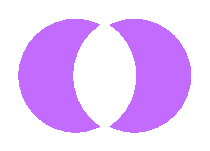
\includegraphics[height=2\baselineskip]{ABSOLUTEPATH/pictures/light-mode/symmetric-difference/via-unions-and-intersections/Venn0110.pdf}}}%
                    \hspace{0.5em}\scalebox{1.5}{$\mathbin{=}$}\hspace{0.5em}%
                    \underset{\scalebox{1.0}{$U\cup V$}}{\raisebox{-0.4\height}{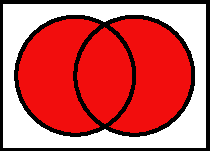
\includegraphics[height=2\baselineskip]{ABSOLUTEPATH/pictures/light-mode/symmetric-difference/via-unions-and-intersections/Venn0111.pdf}}}%
                    \hspace{0.5em}\scalebox{1.5}{$\mathbin{\setminus}$}\hspace{0.5em}%
                    \underset{\scalebox{1.0}{$U\cap V$}}{\raisebox{-0.4\height}{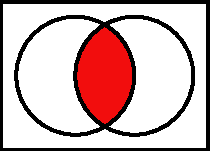
\includegraphics[height=2\baselineskip]{ABSOLUTEPATH/pictures/light-mode/symmetric-difference/via-unions-and-intersections/Venn0001.pdf}}}%
                    .%
                \end{webcompile}%%
                \par\vspace*{-0.5\baselineskip}
            }%
            %---  End Footnote  ---%
            \[
                U\sdiff V
                =
                (U\cup V)%
                \setminus%
                (U\cap V)%
            \]%
            for each $X\in\Obj(\Sets)$ and each $U,V\in\mathcal{P}(X)$.
        \item\label{properties-of-symmetric-differences-associativity}\SloganFont{Associativity. }We have%
            %--- Begin Footnote ---%
            \footnote{%
                \SloganFont{Illustration: }
                \begin{webcompile}
                    \underset{\scalebox{1.0}{$U\sdiff V$}}{\raisebox{-0.4\height}{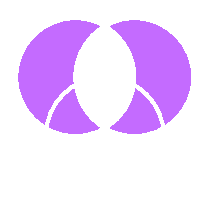
\includegraphics[height=3\baselineskip]{ABSOLUTEPATH/pictures/light-mode/symmetric-difference/associativity/A_sdiff_B.pdf}}}%
                    \hspace{0.5em}\scalebox{1.5}{$\mathbin{\sdiff}$}\hspace{0.5em}%
                    \underset{\mcp{\scalebox{1.0}{$W$}}}{\raisebox{-0.4\height}{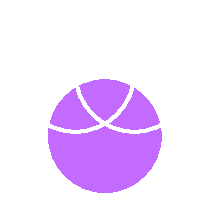
\includegraphics[height=3\baselineskip]{ABSOLUTEPATH/pictures/light-mode/symmetric-difference/associativity/C.pdf}}}%
                    \hspace{0.5em}\scalebox{1.5}{$\mathbin{=}$}\hspace{0.5em}%
                    \underset{\scalebox{1.0}{$U\sdiff V\sdiff W$}}{\raisebox{-0.4\height}{
\includegraphics[height=3\baselineskip]{ABSOLUTEPATH/pictures/light-mode/symmetric-difference/associativity/A_sdiff_B_sdiff_C.pdf}}}%
                    \hspace{0.5em}\scalebox{1.5}{$\mathbin{=}$}\hspace{0.5em}%
                    \underset{\mcp{\scalebox{1.0}{$U$}}}{\raisebox{-0.4\height}{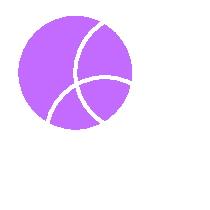
\includegraphics[height=3\baselineskip]{ABSOLUTEPATH/pictures/light-mode/symmetric-difference/associativity/A.pdf}}}%
                    \hspace{0.5em}\scalebox{1.5}{$\mathbin{\sdiff}$}\hspace{0.5em}%
                    \underset{\scalebox{1.0}{$V\sdiff W$}}{\raisebox{-0.4\height}{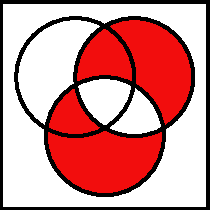
\includegraphics[height=3\baselineskip]{ABSOLUTEPATH/pictures/light-mode/symmetric-difference/associativity/B_sdiff_C.pdf}}}%
                    .%
                \end{webcompile}%%
                \par\vspace*{-0.375\baselineskip}
            }%
            %---  End Footnote  ---%
            \[
                (U\sdiff V)\sdiff W
                =
                U\sdiff(V\sdiff W)
            \]%
            for each $X\in\Obj(\Sets)$ and each $U,V,W\in\mathcal{P}(X)$.
        \item\label{properties-of-symmetric-differences-commutativity}\SloganFont{Commutativity. }We have
            \[
                U\sdiff V
                =
                V\sdiff U
            \]%
            for each $X\in\Obj(\Sets)$ and each $U,V\in\mathcal{P}(X)$.
        \item\label{properties-of-symmetric-differences-unitality}\SloganFont{Unitality. }We have
            \begin{align*}
                U\sdiff\emptyset  &= U,\\
                \emptyset\sdiff U &= U
            \end{align*}
            for each $X\in\Obj(\Sets)$ and each $U\in\mathcal{P}(X)$.
        \item\label{properties-of-symmetric-differences-invertibility}\SloganFont{Invertibility. }We have
            \[
                U\sdiff U
                =
                \emptyset
            \]%
            for each $X\in\Obj(\Sets)$ and each $U\in\mathcal{P}(X)$.
        \item\label{properties-of-symmetric-differences-interaction-with-unions}\SloganFont{Interaction With Unions. }We have
            \[
                (U\sdiff V)\cup(V\sdiff T)
                =
                (U\cup V\cup W)\setminus(U\cap V\cap W)
            \]%
            for each $X\in\Obj(\Sets)$ and each $U,V,W\in\mathcal{P}(X)$.
        \item\label{properties-of-symmetric-differences-interaction-with-complements-1}\SloganFont{Interaction With Complements I. }We have
            \[
                U\sdiff U^{\sfc}%
                =
                X%
            \]%
            for each $X\in\Obj(\Sets)$ and each $U\in\mathcal{P}(X)$.
        \item\label{properties-of-symmetric-differences-interaction-with-complements-2}\SloganFont{Interaction With Complements II. }We have
            \begin{align*}
                U\sdiff X &= U^{\sfc},\\%
                X\sdiff U &= U^{\sfc}%
            \end{align*}
            for each $X\in\Obj(\Sets)$ and each $U\in\mathcal{P}(X)$.
        \item\label{properties-of-symmetric-differences-interaction-with-complements-3}\SloganFont{Interaction With Complements III. }We have
            \[
                U^{\sfc}\sdiff V^{\sfc}%
                =%
                U\sdiff V%
            \]%
            for each $X\in\Obj(\Sets)$ and each $U,V\in\mathcal{P}(X)$.
        \item\label{properties-of-symmetric-differences-transitivity}\SloganFont{``Transitivity''. }We have
            \[
                (U\sdiff V)\sdiff(V\sdiff W)%
                =%
                U\sdiff W%
            \]%
            for each $X\in\Obj(\Sets)$ and each $U,V,W\in\mathcal{P}(X)$.
        \item\label{properties-of-symmetric-differences-the-triangle-inequality-for-symmetric-differences}\SloganFont{The Triangle Inequality for Symmetric Differences. }We have
            \[
                U\sdiff W%
                \subset%
                U\sdiff V%
                \cup
                V\sdiff W%
            \]%
            for each $X\in\Obj(\Sets)$ and each $U,V,W\in\mathcal{P}(X)$.
        \item\label{properties-of-symmetric-differences-distributivity-over-intersections}\SloganFont{Distributivity Over Intersections. }We have
            \begin{align*}
                U\cap(V\sdiff W)  &= (U\cap V)\sdiff(U\cap W),\\
                (U\sdiff V)\cap W &= (U\cap W)\sdiff(V\cap W)
            \end{align*}
            for each $X\in\Obj(\Sets)$ and each $U,V,W\in\mathcal{P}(X)$.
        \item\label{properties-of-symmetric-differences-interaction-with-characteristic-functions}\SloganFont{Interaction With Characteristic Functions. }We have
            \[
                \chi_{U\sdiff V}%
                =%
                \chi_{U}%
                +%
                \chi_{V}%
                -%
                2\chi_{U\cap V}%
            \]%
            and thus, in particular, we have
            \[
                \chi_{U\sdiff V}%
                \equiv%
                \chi_{U}+\chi_{V}%
                \mod{2}%
            \]%
            for each $X\in\Obj(\Sets)$ and each $U,V\in\mathcal{P}(X)$.
        \item\label{properties-of-symmetric-differences-bijectivity}\SloganFont{Bijectivity. }Given $A,B\subset\mathcal{P}(X)$, the maps
            \begin{align*}
                A\sdiff-  &\colon \mathcal{P}(X) \to \mathcal{P}(X),\\
                -\sdiff B &\colon \mathcal{P}(X) \to \mathcal{P}(X)
            \end{align*}
            are bijections with inverses given by
            \begin{align*}
                (A\sdiff-)^{-1}  &= -\cup(A\cap-),\\
                (-\sdiff B)^{-1} &= -\cup(B\cap-).
            \end{align*}
            Moreover, the map
            \[
                C\mapsto C\sdiff(A\sdiff B)%
            \]%
            is a bijection of $\mathcal{P}(X)$ onto itself sending $A$ to $B$ and $B$ to $A$.
        \item\label{properties-of-symmetric-differences-interaction-with-powersets-and-groups}\SloganFont{Interaction With Powersets and Groups. }Let $X$ be a set.
            \begin{enumerate}
                \item\label{properties-of-symmetric-differences-interaction-with-powersets-and-groups-a}The quadruple $(\mathcal{P}(X),\sdiff,\emptyset,\id_{\mathcal{P}(X)})$ is an abelian group.%
                    %--- Begin Footnote ---%
                    \footnote{%
                        Here are some examples:
                        \begin{enumerate}
                            \item When $X=\emptyset$, we have an isomorphism of groups between $\mathcal{P}(\emptyset)$ and the trivial group:
                                \[
                                    (\mathcal{P}(\emptyset),\sdiff,\emptyset,\id_{\mathcal{P}(\emptyset)})
                                    \cong
                                    \pt.
                                \]%
                            \item When $X=\pt$, we have an isomorphism of groups between $\mathcal{P}(\pt)$ and $\Zn{2}$:
                                \[
                                    (\mathcal{P}(\pt),\sdiff,\emptyset,\id_{\mathcal{P}(\pt)})
                                    \cong
                                    \Zn{2}.
                                \]%
                            \item When $X=\{0,1\}$, we have an isomorphism of groups between $\mathcal{P}(\{0,1\})$ and $\Zn{2}\times\Zn{2}$:
                                \[
                                    (\mathcal{P}(\{0,1\}),\sdiff,\emptyset,\id_{\mathcal{P}(\{0,1\})})
                                    \cong
                                    \Zn{2}\times\Zn{2}.
                                \]%
                        \end{enumerate}
                        \par\vspace*{-1.5\baselineskip}
                    }%
                    %---  End Footnote  ---%
                \item\label{properties-of-symmetric-differences-interaction-with-powersets-and-groups-b}Every element of $\mathcal{P}(X)$ has order $2$ with respect to $\sdiff$, and thus $\mathcal{P}(X)$ is a \emph{Boolean group} (i.e.\ an abelian $2$-group).
            \end{enumerate}
        \item\label{properties-of-symmetric-differences-interaction-with-powersets-and-vector-spaces-1}\SloganFont{Interaction With Powersets and Vector Spaces I. }The pair $(\mathcal{P}(X),\alpha_{\mathcal{P}(X)})$ consisting of
            \begin{itemize}
                \item The group $\mathcal{P}(X)$ of \cref{properties-of-symmetric-differences-interaction-with-powersets-and-groups-1};
                \item The map $\alpha_{\mathcal{P}(X)}\colon\F_{2}\times\mathcal{P}(X)\to\mathcal{P}(X)$ defined by
                    \begin{align*}
                        0\cdot U &\defeq \emptyset,\\
                        1\cdot U &\defeq U;
                    \end{align*}
            \end{itemize}
            is an $\F_{2}$-vector space.
        \item\label{properties-of-symmetric-differences-interaction-with-powersets-and-vector-spaces-2}\SloganFont{Interaction With Powersets and Vector Spaces II. }If $X$ is finite, then:
            \begin{enumerate}% PROCESS %
                \item The set of singletons sets on the elements of $X$ forms a basis for the $\F_{2}$-vector space $(\mathcal{P}(X),\alpha_{\mathcal{P}(X)})$ of \cref{properties-of-symmetric-differences-interaction-with-powersets-and-vector-spaces-1}.
                \item We have
                    \[
                        \dim(\mathcal{P}(X))%
                        =%
                        \#\mathcal{P}(X).%
                    \]%
            \end{enumerate}% PROCESS %
        \item\label{properties-of-symmetric-differences-interaction-with-powersets-and-rings}\SloganFont{Interaction With Powersets and Rings. }The quintuple $(\mathcal{P}(X),\sdiff,\cap,\emptyset,X)$ is a commutative ring.%
            %--- Begin Footnote ---%
            \footnote{%
                \textdbend\SloganFont{Warning: }The analogous statement replacing intersections by unions (i.e.\ that the quintuple $(\mathcal{P}(X),\sdiff,\cup,\emptyset,X)$ is a ring) is false, however. See \cite{proof-wiki:symmetric-difference-with-union-does-not-form-ring} for a proof.

                END TEXTDBEND
                \par\vspace*{-1.75\baselineskip}
            }%
            %---  End Footnote  ---%
        %\item\label{properties-of-symmetric-differences-}\SloganFont{. }
    \end{enumerate}
\end{proposition}
\begin{Proof}{Proof of \cref{properties-of-symmetric-differences}}%
    \FirstProofBox{\cref{properties-of-symmetric-differences-lack-of-functoriality}: Lack of Functoriality}%
    Omitted.

    \ProofBox{\cref{properties-of-symmetric-differences-via-unions-and-intersections}: Via Unions and Intersections}%
    See \cite{proof-wiki:equivalence-of-definitions-of-symmetric-difference}.

    \ProofBox{\cref{properties-of-symmetric-differences-associativity}: Associativity}%
    See \cite{proof-wiki:symmetric-difference-is-associative}.

    \ProofBox{\cref{properties-of-symmetric-differences-commutativity}: Commutativity}%
    See \cite{proof-wiki:symmetric-difference-is-commutative}.

    \ProofBox{\cref{properties-of-symmetric-differences-unitality}: Unitality}%
    This follows from \cref{properties-of-symmetric-differences-commutativity} and \cite{proof-wiki:symmetric-difference-with-empty-set}.

    \ProofBox{\cref{properties-of-symmetric-differences-invertibility}: Invertibility}%
    See \cite{proof-wiki:symmetric-difference-with-self-is-empty-set}.

    \ProofBox{\cref{properties-of-symmetric-differences-interaction-with-unions}: Interaction With Unions}%
    See \cite{proof-wiki:union-of-symmetric-differences}.

    \ProofBox{\cref{properties-of-symmetric-differences-interaction-with-complements-1}: Interaction With Complements I}%
    See \cite{proof-wiki:symmetric-difference-with-complement}.

    \ProofBox{\cref{properties-of-symmetric-differences-interaction-with-complements-2}: Interaction With Complements II}%
    This follows from \cref{properties-of-symmetric-differences-commutativity} and \cite{proof-wiki:symmetric-difference-with-universe}.

    \ProofBox{\cref{properties-of-symmetric-differences-interaction-with-complements-3}: Interaction With Complements III}%
    See \cite{proof-wiki:symmetric-difference-of-complements}.

    \ProofBox{\cref{properties-of-symmetric-differences-transitivity}: ``Transitivity''}%
    We have
    % BEGIN RAW HTML %
    <div class="math-content">
        <div class="math-wrapper">
            <p>$(U\sdiff V)\sdiff(V\sdiff W) = U\sdiff(V\sdiff(V\sdiff W))$</p>
            <p class="ptag">(by \cref{properties-of-symmetric-differences-associativity})</p>
        </div>
    </div>

    <div class="math-content">
        <div class="math-wrapper">
        <p>$\phantom{(U\sdiff V)\sdiff(V\sdiff W)} =\rlap{U\sdiff((V\sdiff V)\sdiff W)}\phantom{U\sdiff(V\sdiff(V\sdiff W))}$</p>
            <p class="ptag">(by \cref{properties-of-symmetric-differences-associativity})</p>
        </div>
    </div>

    <div class="math-content">
        <div class="math-wrapper">
            <p>$\phantom{(U\sdiff V)\sdiff(V\sdiff W)} = \rlap{U\sdiff(\emptyset\sdiff W)}\phantom{U\sdiff(V\sdiff(V\sdiff W))}$</p>
            <p class="ptag">(by \cref{properties-of-symmetric-differences-invertibility})</p>
        </div>
    </div>

    <div class="math-content">
        <div class="math-wrapper">
            <p>$\phantom{(U\sdiff V)\sdiff(V\sdiff W)} = \rlap{U\sdiff W}\phantom{U\sdiff(V\sdiff(V\sdiff W))}$</p>
            <p class="ptag">(by \cref{properties-of-symmetric-differences-unitality})</p>
        </div>
    </div>
    % BEGIN LATEX HTML %
    \begin{align*}
        (U\sdiff V)\sdiff(V\sdiff W) &= U\sdiff(V\sdiff(V\sdiff W))  \ptag{by \cref{properties-of-symmetric-differences-associativity}}\\
                                     &= U\sdiff((V\sdiff V)\sdiff W) \ptag{by \cref{properties-of-symmetric-differences-associativity}}\\
                                     &= U\sdiff(\emptyset\sdiff W)   \ptag{by \cref{properties-of-symmetric-differences-invertibility}}\\
                                     &= U\sdiff W                    \ptag{by \cref{properties-of-symmetric-differences-unitality}}
    \end{align*}
    % END RAW HTML %

    \ProofBox{\cref{properties-of-symmetric-differences-the-triangle-inequality-for-symmetric-differences}: The Triangle Inequality for Symmetric Differences}%
    This follows from \cref{properties-of-symmetric-differences-transitivity,properties-of-symmetric-differences-via-unions-and-intersections}.

    \ProofBox{\cref{properties-of-symmetric-differences-distributivity-over-intersections}: Distributivity Over Intersections}%
    See \cite{proof-wiki:intersection-distributes-over-symmetric-difference}.

    \ProofBox{\cref{properties-of-symmetric-differences-interaction-with-characteristic-functions}: Interaction With Characteristic Functions}%
    See \cite{proof-wiki:characteristic-function-of-symmetric-difference}.

    \ProofBox{\cref{properties-of-symmetric-differences-bijectivity}: Bijectivity}%
    Clear.

    \ProofBox{\cref{properties-of-symmetric-differences-interaction-with-powersets-and-groups}: Interaction With Powersets and Groups}%
    \cref{properties-of-symmetric-differences-interaction-with-powersets-and-groups-a} follows from%
    %--- Begin Footnote ---%
    \footnote{%
        Reference: \cite{proof-wiki:symmetric-difference-on-power-set-forms-abelian-group}.
    } %
    %---  End Footnote  ---%
    \cref{properties-of-symmetric-differences-associativity,properties-of-symmetric-differences-unitality,properties-of-symmetric-differences-invertibility,properties-of-symmetric-differences-commutativity}, while \cref{properties-of-symmetric-differences-interaction-with-powersets-and-groups-b} follows from \cref{properties-of-symmetric-differences-invertibility}.

    \ProofBox{\cref{properties-of-symmetric-differences-interaction-with-powersets-and-vector-spaces-1}: Interaction With Powersets and Vector Spaces I}%
    Clear.

    \ProofBox{\cref{properties-of-symmetric-differences-interaction-with-powersets-and-vector-spaces-2}: Interaction With Powersets and Vector Spaces II}%
    Omitted.

    \ProofBox{\cref{properties-of-symmetric-differences-interaction-with-powersets-and-rings}: Interaction With Powersets and Rings}%
    This follows from \cref{properties-of-binary-intersections-annihilation-with-the-empty-set,properties-of-binary-intersections-interaction-with-powersets-and-monoids-with-zero} of \cref{properties-of-binary-intersections} and \cref{properties-of-symmetric-differences-distributivity-over-intersections,properties-of-symmetric-differences-interaction-with-powersets-and-groups}.%
    %--- Begin Footnote ---%
    \footnote{%
        \SloganFont{Reference: }\cite{proof-wiki:symmetric-difference-with-intersection-forms-ring}.
        \par\vspace*{-1.75\baselineskip}
    }%
    %---  End Footnote  ---%
\end{Proof}
\section{Powersets}\label{section-powersets}
\subsection{Characteristic Functions}\label{subsection-characteristic-functions}
Let $X$ be a set.
\begin{definition}{Characteristic Functions}{characteristic-functions}%
    Let $U\subset X$ and let $x\in X$.%
    \begin{enumerate}
        \item\label{characteristic-functions-characteristic-function-of-u}The \index[set-theory]{characteristic function!of a set}\textbf{characteristic function of $U$}%
            %--- Begin Footnote ---%
            \footnote{%
                \SloganFont{Further Terminology: }Also called the \index[set-theory]{indicator function|see {characteristic function}}\textbf{indicator function of $U$}.
            } %
            %---  End Footnote  ---%
            is the function\index[notation]{chiU@$\chi_{U}$}%
            %--- Begin Footnote ---%
            \footnote{%
                \SloganFont{Further Notation: }Also written \index[notation]{chiXU@$\chi_{X}(U,-)$}$\chi_{X}(U,-)$ or \index[notation]{chiXU@$\chi_{X}(-,U)$}$\chi_{X}(-,U)$.
            }%
            %---  End Footnote  ---%
            \[%
                \chi_{U}%
                \colon%
                X%
                \to%
                \TTV%
            \]%
            defined by
            \[
                \chi_{U}(x)
                \defeq
                \begin{cases}
                    \true  &\text{if $x\in U$,}\\
                    \false &\text{if $x\nin U$}
                \end{cases}
            \]%
            for each $x\in X$.
        \item\label{characteristic-functions-characteristic-function-of-x}The \index[set-theory]{characteristic function!of an element}\textbf{characteristic function of $x$} is the function\index[notation]{chix@$\chi_{x}$}%
            %--- Begin Footnote ---%
            \footnote{%
                \SloganFont{Further Notation: }Also written \index[notation]{chix@$\chi^{x}$}$\chi^{x}$, \index[notation]{chiXx@$\chi_{X}(x,-)$}$\chi_{X}(x,-)$, or \index[notation]{chiXU@$\chi_{X}(-,x)$}$\chi_{X}(-,x)$.
            }%
            %---  End Footnote  ---%
            \[%
                \chi_{x}%
                \colon%
                X%
                \to%
                \TTV%
            \]%
            defined by%
            \[
                \chi_{x}
                \defeq
                \chi_{\{x\}},%
            \]%
            i.e.\ by%
            \[
                \chi_{x}(y)
                \defeq
                \begin{cases}
                    \true  &\text{if $x=y$,}\\
                    \false &\text{if $x\neq y$}
                \end{cases}
            \]%
            for each $y\in X$.
        \item\label{characteristic-functions-characteristic-relation}The \index[set-theory]{characteristic relation}\textbf{characteristic relation on $X$}%
            %--- Begin Footnote ---%
            \footnote{%
                \SloganFont{Further Terminology: }Also called the \textbf{identity relation on $X$}.
            } %
            %---  End Footnote  ---%
            is the relation\index[notation]{chiX12@$\chi_{X}(-_{1},-_{2})$}%
            %--- Begin Footnote ---%
            \footnote{%
                \SloganFont{Further Notation: }Also written \index[notation]{chi12@$\chi^{-_{1}}_{-_{2}}$}$\chi^{-_{1}}_{-_{2}}$, or \index[notation]{simid@$\unsim_{\id}$}$\unsim_{\id}$ in the context of relations.
            }%
            %---  End Footnote  ---%
            \[%
                \chi_{X}(-_{1},-_{2})%
                \colon%
                X\times X%
                \to%
                \TTV%
            \]%
            on $X$ defined by%
            %--- Begin Footnote ---%
            \footnote{%
                As a subset of $X\times X$, the relation $\chi_{X}$ corresponds to the diagonal $\Delta_{X}\subset X\times X$ of $X$.
            }%
            %---  End Footnote  ---%
            \[
                \chi_{X}(x,y)
                \defeq
                \begin{cases}
                    \true  &\text{if $x=y$,}\\
                    \false &\text{if $x\neq y$}
                \end{cases}
            \]%
            for each $x,y\in X$.
        \item\label{characteristic-functions-characteristic-embedding}The \index[set-theory]{characteristic embedding}\textbf{characteristic embedding}%
            %--- Begin Footnote ---%
            \footnote{%
                The name ``characteristic \emph{embedding}'' comes from the fact that there is an analogue of fully faithfulness for $\chi_{(-)}$: given a set $X$, we have
                \[%
                    \Hom_{\mathcal{P}(X)}(\chi_{x},\chi_{y})%
                    =%
                    \chi_{X}(x,y),%
                \]%
                for each $x,y\in X$.
                \par\vspace*{-1.75\baselineskip}
            } %
            %---  End Footnote  ---%
            \textbf{of $X$ into $\mathcal{P}(X)$} is the function\index[notation]{chi@$\chi_{(-)}$}%
            \[%
                \chi_{(-)}%
                \colon%
                X
                \hookrightarrow%
                \mathcal{P}(X)
            \]%
            defined by
            \[
                \chi_{(-)}(x)
                \defeq
                \chi_{x}
            \]%
            for each $x\in X$.
    \end{enumerate}
\end{definition}
\begin{remark}{Characteristic Functions as Decategorifications of Presheaves}{characteristic-functions-as-decategorifications-of-presheaves}%
    The definitions in \cref{characteristic-functions} are decategorifications of co/presheaves, representable co/presheaves, $\Hom$ profunctors, and the Yoneda embedding:%
    %--- Begin Footnote ---%
    \footnote{%
        These statements can be made precise by using the embeddings
        \begin{align*}
            (-)_{\disc} &\colon \Sets       \hookrightarrow \Cats,\\
            (-)_{\disc} &\colon \TTV_{\disc} \hookrightarrow \Sets
        \end{align*}
        of sets into categories and of classical truth values into sets.

        For instance, in this approach the characteristic function
        \[
            \chi_{x}
            \colon
            X
            \to
            \TTV
        \]%
        of an element $x$ of $X$, defined by
        \[
            \chi_{x}(y)
            \defeq
            \begin{cases}
                \true  &\text{if $x=y$,}\\
                \false &\text{if $x\neq y$}
            \end{cases}
        \]%
        for each $y\in X$, is recovered as the representable presheaf
        \[
            \Hom_{X_{\disc}}(-,x)
            \colon
            X_{\disc}
            \to
            \Sets
        \]%
        of the corresponding object $x$ of $X_{\disc}$, defined on objects by
        \[
            \Hom_{X_{\disc}}(y,x)
            \defeq
            \begin{cases}
                \pt       &\text{if $x=y$,}\\
                \emptyset &\text{if $x\neq y$}
            \end{cases}
        \]%
        for each $y\in\Obj(X_{\disc})$.
        \par\vspace*{-1.75\baselineskip}
    }%
    %---  End Footnote  ---%
    \begin{enumerate}
        \item\label{characteristic-functions-as-decategorifications-of-presheaves-functions}A function
            \[
                f\colon X\to\TTV%
            \]%
            is a decategorification of a presheaf%
            \[%
                \SheafFont{F}\colon\CatFont{C}^{\op}\to\Sets,%
            \]%
            with the characteristic functions $\chi_{U}$ of the subsets of $X$ being the primordial examples (and, in fact, all examples) of these.
        \item\label{characteristic-functions-as-decategorifications-of-presheaves-characteristic-functions}The characteristic function%
            \[%
                \chi_{x}%
                \colon%
                X%
                \to%
                \TTV%
            \]%
            of an \emph{element} $x$ of $X$ is a decategorification of the representable presheaf
            \[
                h_{X}%
                \colon%
                \CatFont{C}^{\op}
                \to%
                \Sets%
            \]%
            of an \emph{object} $x$ of a category $\CatFont{C}$.
        \item\label{characteristic-functions-as-decategorifications-of-presheaves-characteristic-relations}The characteristic relation%
            \[%
                \chi_{X}(-_{1},-_{2})%
                \colon%
                X\times X%
                \to%
                \TTV%
            \]%
            of $X$ is a decategorification of the $\Hom$ profunctor
            \[
                \Hom_{\CatFont{C}}(-_{1},-_{2})%
                \colon%
                \CatFont{C}^{\op}\times\CatFont{C}%
                \to%
                \Sets%
            \]%
            of a category $\CatFont{C}$.
        \item\label{characteristic-functions-as-decategorifications-of-presheaves-characteristic-embedding}The characteristic embedding%
            \[
                \chi_{(-)}%
                \colon%
                X%
                \hookrightarrow%
                \mathcal{P}(X)%
            \]%
            of $X$ into $\mathcal{P}(X)$ is a decategorification of the Yoneda embedding
            \[
                \yo%
                \colon%
                \CatFont{C}^{\op}
                \hookrightarrow
                \PSh(\CatFont{C})
            \]%
            of a category $\CatFont{C}$ into $\PSh(\CatFont{C})$.
        \item\label{characteristic-functions-as-decategorifications-of-presheaves-unions-and-colimits}There is also a direct parallel between unions and colimits:
            \begin{itemize}
                \item An element of $\mathcal{P}(X)$    is a union   of elements of $X$,          viewed as one-point     subsets    $\{x\}\in\mathcal{P}(A)$.
                \item An object  of $\PSh(\CatFont{C})$ is a colimit of objects of $\CatFont{C}$, viewed as representable presheaves $h_{X}\in\Obj(\PSh(\CatFont{C}))$.
            \end{itemize}
    \end{enumerate}
\end{remark}
\begin{proposition}{Properties of Characteristic Functions}{properties-of-characteristic-functions}%
    Let $X$ be a set.
    \begin{enumerate}
        \item\label{properties-of-characteristic-functions-the-inclusion-of-characteristic-relations-associated-to-a-function}\SloganFont{The Inclusion of Characteristic Relations Associated to a Function. }Let $f\colon A\to B$ be a function. We have an inclusion%
            %--- Begin Footnote ---%
            \footnote{%
                This is the $0$-categorical version of \ChapterRef{\ChapterCategories, \cref{categories:the-natural-transformation-associated-to-a-functor}}{\cref{the-natural-transformation-associated-to-a-functor}}.
                \par\vspace*{-1.75\baselineskip}
            }%
            %---  End Footnote  ---%
            \begin{webcompile}
                \chi_{B}\circ(f\times f)%
                \subset%
                \chi_{A},%
                \quad%
                \begin{tikzcd}[row sep={4.0*\the\DL,between origins}, column sep={3.0*\the\DL,between origins}, background color=backgroundColor, ampersand replacement=\&]
                    A\times A
                    \arrow[rr,"f\times f"]
                    \arrow[rd,"\chi_{A}"'{pos=0.475},""'{name=1}]
                    \&
                    \&
                    B\times B
                    \arrow[ld,"\chi_{B}"{pos=0.475}]
                    \\
                    \&
                    \TTV\mrp{.}
                    \&
                    % 2-Arrows
                    \arrow[from=1,to=1-3,"\scalebox{1.5}{$\supset$}"{sloped,description,pos=0.575},phantom,shorten <= 0.5em,shorten >= 0.0em]%
                \end{tikzcd}
            \end{webcompile}%
        \item\label{properties-of-characteristic-functions-interaction-with-unions-1}\SloganFont{Interaction With Unions I. }We have
            \[
                \chi_{U\cup V}%
                =%
                \max(\chi_{U},\chi_{V})%
            \]%
            for each $X\in\Obj(\Sets)$ and each $U,V\in\mathcal{P}(X)$.
        \item\label{properties-of-characteristic-functions-interaction-with-unions-2}\SloganFont{Interaction With Unions II. }We have
            \[
                \chi_{U\cup V}%
                =%
                \chi_{U}+\chi_{V}-\chi_{U\cap V}%
            \]%
            for each $X\in\Obj(\Sets)$ and each $U,V\in\mathcal{P}(X)$.
        \item\label{properties-of-characteristic-functions-interaction-with-intersections-1}\SloganFont{Interaction With Intersections I. }We have
            \[
                \chi_{U\cap V}%
                =%
                \chi_{U}\chi_{V}%
            \]%
            for each $X\in\Obj(\Sets)$ and each $U,V\in\mathcal{P}(X)$.
        \item\label{properties-of-characteristic-functions-interaction-with-intersections-2}\SloganFont{Interaction With Intersections II. }We have
            \[
                \chi_{U\cap V}%
                =%
                \min(\chi_{U},\chi_{V})%
            \]%
            for each $X\in\Obj(\Sets)$ and each $U,V\in\mathcal{P}(X)$.
        \item\label{properties-of-characteristic-functions-interaction-with-differences}\SloganFont{Interaction With Differences. }We have
            \[
                \chi_{U\setminus V}%
                =%
                \chi_{U}%
                -%
                \chi_{U\cap V}%
            \]%
            for each $X\in\Obj(\Sets)$ and each $U,V\in\mathcal{P}(X)$.
        \item\label{properties-of-characteristic-functions-interaction-with-complements}\SloganFont{Interaction With Complements. }We have
            \[
                \chi_{U^{\sfc}}%
                =%
                1-\chi_{U}%
            \]%
            for each $X\in\Obj(\Sets)$ and each $U\in\mathcal{P}(X)$.
        \item\label{properties-of-characteristic-functions-interaction-with-symmetric-differences}\SloganFont{Interaction With Symmetric Differences. }We have
            \[
                \chi_{U\sdiff V}%
                =%
                \chi_{U}%
                +%
                \chi_{V}%
                -%
                2\chi_{U\cap V}%
            \]%
            and thus, in particular, we have
            \[
                \chi_{U\sdiff V}%
                \equiv%
                \chi_{U}+\chi_{V}%
                \mod{2}%
            \]%
            for each $X\in\Obj(\Sets)$ and each $U,V\in\mathcal{P}(X)$.
        \item\label{properties-of-characteristic-functions-interaction-between-the-characteristic-embedding-and-morphisms}\SloganFont{Interaction Between the Characteristic Embedding and Morphisms. }Let $f\colon X\to Y$ be a map of sets. The diagram
            \begin{webcompile}
                f_{*}\circ\chi_{X}%
                =%
                \chi_{X'}\circ f,%
                \qquad%
                \begin{tikzcd}[row sep={5.0*\the\DL,between origins}, column sep={5.5*\the\DL,between origins}, background color=backgroundColor, ampersand replacement=\&]
                    X
                    \arrow[r,"f"]
                    \arrow[d,"\chi_{X}"']
                    \&
                    X'
                    \arrow[d,"\chi_{X'}"]
                    \\
                    \mathcal{P}(X)
                    \arrow[r,"f_{*}"']
                    \&
                    \mathcal{P}(X')\mrp{.}
                \end{tikzcd}
            \end{webcompile}
            commutes.
        %\item\label{properties-of-characteristic-functions-}\SloganFont{. }
    \end{enumerate}
\end{proposition}
\begin{Proof}{Proof of \cref{properties-of-characteristic-functions}}%
    \FirstProofBox{\cref{properties-of-characteristic-functions-the-inclusion-of-characteristic-relations-associated-to-a-function}: The Inclusion of Characteristic Relations Associated to a Function}%
    The inclusion $\chi_{B}(f(a),f(b))\subset\chi_{A}(a,b)$ is equivalent to the statement \say{if $a=b$, then $f(a)=f(b)$}, which is true.

    \ProofBox{\cref{properties-of-characteristic-functions-interaction-with-unions-1}: Interaction With Unions I}%
    This is a repetition of \cref{properties-of-binary-unions-interaction-with-characteristic-functions-1} of \cref{properties-of-binary-unions} and is proved there.

    \ProofBox{\cref{properties-of-characteristic-functions-interaction-with-unions-2}: Interaction With Unions II}%
    This is a repetition of \cref{properties-of-binary-unions-interaction-with-characteristic-functions-2} of \cref{properties-of-binary-unions} and is proved there.

    \ProofBox{\cref{properties-of-characteristic-functions-interaction-with-intersections-1}: Interaction With Intersections I}%
    This is a repetition of \cref{properties-of-binary-intersections-interaction-with-characteristic-functions-1} of \cref{properties-of-binary-intersections} and is proved there.

    \ProofBox{\cref{properties-of-characteristic-functions-interaction-with-intersections-2}: Interaction With Intersections II}%
    This is a repetition of \cref{properties-of-binary-intersections-interaction-with-characteristic-functions-2} of \cref{properties-of-binary-intersections} and is proved there.

    \ProofBox{\cref{properties-of-characteristic-functions-interaction-with-differences}: Interaction With Differences}%
    This is a repetition of \cref{properties-of-differences-interaction-with-characteristic-functions} of \cref{properties-of-differences} and is proved there.

    \ProofBox{\cref{properties-of-characteristic-functions-interaction-with-complements}: Interaction With Complements}%
    This is a repetition of \cref{properties-of-complements-interaction-with-characteristic-functions} of \cref{properties-of-complements} and is proved there.

    \ProofBox{\cref{properties-of-characteristic-functions-interaction-with-symmetric-differences}: Interaction With Symmetric Differences}%
    This is a repetition of \cref{properties-of-symmetric-differences-interaction-with-characteristic-functions} of \cref{properties-of-symmetric-differences} and is proved there.

    \ProofBox{\cref{properties-of-characteristic-functions-interaction-between-the-characteristic-embedding-and-morphisms}: Interaction Between the Characteristic Embedding and Morphisms}%
    Indeed, we have
    \begin{align*}
        [f_{*}\circ\chi_{X}](x) &\defeq f_{*}(\chi_{X}(x))\\%
                                &\defeq f_{*}(\{x\})\\%
                                &=      \{f(x)\}\\%
                                &\defeq \chi_{X'}(f(x))\\%
                                &\defeq [\chi_{X'}\circ f](x),%
    \end{align*}
    for each $x\in X$, showing the desired equality.
\end{Proof}
\subsection{The Yoneda Lemma for Sets}\label{subsection-the-yoneda-lemma-for-sets}
Let $X$ be a set and let $U\subset X$ be a subset of $X$.%
\begin{proposition}{The Yoneda Lemma for Sets}{the-yoneda-lemma-for-sets}%
    We have
    \[
        \chi_{\mathcal{P}(X)}(\chi_{x},\chi_{U})%
        =%
        \chi_{U}(x)%
    \]%
    for each $x\in X$, giving an equality of functions
    \[
        \chi_{\mathcal{P}(X)}(\chi_{(-)},\chi_{U})%
        =%
        \chi_{U}.%
    \]%
\end{proposition}
\begin{Proof}{Proof of \cref{the-yoneda-lemma-for-sets}}%
    Clear.
\end{Proof}
\begin{corollary}{The Characteristic Embedding Is Fully Faithful}{the-characteristic-embedding-is-fully-faithful}%
    The characteristic embedding is fully faithful, i.e., we have
    \[
        \chi_{\mathcal{P}(X)}(\chi_{x},\chi_{y})%
        =%
        \chi_{X}(x,y)
    \]%
    for each $x,y\in X$.
\end{corollary}
\begin{Proof}{Proof of \cref{the-characteristic-embedding-is-fully-faithful}}%
    This follows from \cref{the-yoneda-lemma-for-sets}.
\end{Proof}
\subsection{Powersets}\label{subsection-powersets}
Let $X$ be a set.%
\begin{definition}{Powersets}{powersets}%
    The \index[set-theory]{powerset}\textbf{powerset of $X$} is the set \index[notation]{PX@$\mathcal{P}(X)$}$\mathcal{P}(X)$ defined by
    \[
        \mathcal{P}(X)
        \defeq
        \{%
            U\in P%
            \ \middle|\ %
            U\subset X%
        \},
    \]%
    where $P$ is the set in the axiom of powerset, \cref{zermelo-fraenkel-set-theory-the-axiom-of-powerset} of \cref{zermelo-fraenkel-set-theory}.
\end{definition}
\begin{remark}{Powersets as Decategorifications of Co/Presheaf Categories}{powersets-as-decategorifications-of-co-presheaf-categories}%
    The powerset of a set is a decategorification of the category of presheaves of a category: while%
    %--- Begin Footnote ---%
    \footnote{%
        This parallel is based on the following comparison:
        \begin{itemize}
            \item A category is enriched over the category
                \[
                    \Sets%
                    \defeq%
                    \ZeroCats%
                \]%
                of sets (i.e.\ ``$0$-categories''), with presheaves taking values on it.
            \item A set is enriched over the set
                \[
                    \TTV%
                    \defeq%
                    \MinusOneCats%
                \]%
                of classical truth values (i.e.\ ``$(-1)$-categories''), with characteristic functions taking values on it.
        \end{itemize}
        \par\vspace*{-1.75\baselineskip}
    }%
    %---  End Footnote  ---%
    \begin{itemize}
        \item The powerset of a set $X$ is equivalently (\cref{properties-of-powersets-as-sets-of-functions-relations-powersets-as-sets-of-functions-1,properties-of-powersets-as-sets-of-functions-relations-powersets-as-sets-of-functions-2} of \cref{properties-of-powersets-as-sets-of-functions-relations}) the set
            \[%
                \Sets(X,\TTV)
            \]%
            of functions from $X$ to the set $\TTV$ of classical truth values.
        \item The category of presheaves on a category $\CatFont{C}$ is the category
            \[%
                \Fun(\CatFont{C}^{\op},\Sets)%
            \]%
            of functors from $\CatFont{C}^{\op}$ to the category $\Sets$ of sets.
    \end{itemize}
\end{remark}
\begin{proposition}{Properties of Powersets: As Categories}{properties-of-powersets-as-categories}%
    Let $X$ be a set.
    \begin{enumerate}
        \item\label{properties-of-powersets-as-categories-co-completeness}\SloganFont{Co/Completeness. }The (posetal) category (associated to) $(\mathcal{P}(X),\subset)$ is complete and cocomplete:
            \begin{enumerate}
                \item\SloganFont{Products. }The products in $\mathcal{P}(X)$ are given by intersection of subsets.
                \item\SloganFont{Coproducts. }The coproducts in $\mathcal{P}(X)$ are given by union of subsets.
                \item\SloganFont{Co/Equalisers. }Being a posetal category, $\mathcal{P}(X)$ only has at most one morphisms between any two objects, so co/equalisers are trivial.
            \end{enumerate}
        \item\label{properties-of-powersets-as-categories-cartesian-closedness}\SloganFont{Cartesian Closedness. }The category $\mathcal{P}(X)$ is Cartesian closed with internal Hom
            \[
                \eHom_{\mathcal{P}(X)}(-_{1},-_{2})%
                \colon
                \mathcal{P}(X)\opsup\times\mathcal{P}(X)
                \to
                \mathcal{P}(X)
            \]%
            given by%
            %--- Begin Footnote ---%
            \footnote{%
                For intuition regarding the expression defining $\eHom_{\mathcal{P}(X)}(U,V)$, see \cref{intuition-for-the-internal-hom-of-px}.
                \par\vspace*{-1.75\baselineskip}
            }%
            %---  End Footnote  ---%
            \[
                \eHom_{\mathcal{P}(X)}(U,V)%
                \defeq
                (X\setminus U)\cup V
            \]%
            for each $U,V\in\Obj(\mathcal{P}(X))$.
        %\item\label{properties-of-powersets-as-categories-}\SloganFont{. }
    \end{enumerate}
\end{proposition}
\begin{Proof}{Proof of \cref{properties-of-powersets-as-categories}}%
    \FirstProofBox{\cref{properties-of-powersets-as-categories-co-completeness}: Co/Completeness}%
    Clear.

    \ProofBox{\cref{properties-of-powersets-as-categories-cartesian-closedness}: Cartesian Closedness}%
    This follows from \cref{properties-of-binary-intersections-adjointness} of \cref{properties-of-binary-intersections}.
\end{Proof}
\begin{proposition}{Properties of Powersets: Functoriality and Adjointness}{properties-of-powersets-functoriality-and-adjointness}%
    Let $X$ be a set.
    \begin{enumerate}
        \item\label{properties-of-powersets-functoriality-and-adjointness-functoriality-1}\SloganFont{Functoriality \rmI. }The assignment $X\mapsto\mathcal{P}(X)$ defines a functor\index[notation]{Pstar@$\mathcal{P}_{*}$}
            \[
                \mathcal{P}_{*}%
                \colon%
                \Sets%
                \to%
                \Sets,%
            \]%
            where
            \begin{itemize}
                \item\SloganFont{Action on Objects. }For each $A\in\Obj(\Sets)$, we have
                    \[
                        \mathcal{P}_{*}(A)%
                        \defeq%
                        \mathcal{P}(A).%
                    \]%
                \item\SloganFont{Action on Morphisms. }For each $A,B\in\Obj(\Sets)$, the action on morphisms
                    \[
                        \mathcal{P}_{*|A,B}%
                        \colon%
                        \Sets(A,B)%
                        \to%
                        \Sets(\mathcal{P}(A),\mathcal{P}(B))%
                    \]%
                    of $\mathcal{P}_{*}$ at $(A,B)$ is the map defined by by sending a map of sets $f\colon A\to B$ to the map
                    \[
                        \mathcal{P}_{*}(f)%
                        \colon%
                        \mathcal{P}(A)%
                        \to%
                        \mathcal{P}(B)%
                    \]%
                    defined by
                    \[
                        \mathcal{P}_{*}(f)%
                        \defeq%
                        f_{*},%
                    \]%
                    as in \cref{the-direct-image-function-associated-to-a-function}.
            \end{itemize}
        \item\label{properties-of-powersets-functoriality-and-adjointness-functoriality-2}\SloganFont{Functoriality \rmII. }The assignment $X\mapsto\mathcal{P}(X)$ defines a functor\index[notation]{Pminusone@$\mathcal{P}^{-1}$}
            \[
                \mathcal{P}^{-1}%
                \colon%
                \Sets^{\op}%
                \to%
                \Sets,%
            \]%
            where
            \begin{itemize}
                \item\SloganFont{Action on Objects. }For each $A\in\Obj(\Sets)$, we have
                    \[
                        \mathcal{P}^{-1}(A)%
                        \defeq%
                        \mathcal{P}(A).%
                    \]%
                \item\SloganFont{Action on Morphisms. }For each $A,B\in\Obj(\Sets)$, the action on morphisms
                    \[
                        \mathcal{P}^{-1}_{A,B}%
                        \colon%
                        \Sets(A,B)%
                        \to%
                        \Sets(\mathcal{P}(B),\mathcal{P}(A))%
                    \]%
                    of $\mathcal{P}^{-1}$ at $(A,B)$ is the map defined by by sending a map of sets $f\colon A\to B$ to the map
                    \[
                        \mathcal{P}^{-1}(f)%
                        \colon%
                        \mathcal{P}(B)%
                        \to%
                        \mathcal{P}(A)%
                    \]%
                    defined by
                    \[
                        \mathcal{P}^{-1}(f)%
                        \defeq%
                        f^{-1},%
                    \]%
                    as in \cref{the-inverse-image-function-associated-to-a-function}.
            \end{itemize}
        \item\label{properties-of-powersets-functoriality-and-adjointness-functoriality-3}\SloganFont{Functoriality \rmIII. }The assignment $X\mapsto\mathcal{P}(X)$ defines a functor\index[notation]{Pshriek@$\mathcal{P}_{"!}$}
            \[
                \mathcal{P}_{!}%
                \colon%
                \Sets%
                \to%
                \Sets,%
            \]%
            where
            \begin{itemize}
                \item\SloganFont{Action on Objects. }For each $A\in\Obj(\Sets)$, we have
                    \[
                        \mathcal{P}_{!}(A)%
                        \defeq%
                        \mathcal{P}(A).%
                    \]%
                \item\SloganFont{Action on Morphisms. }For each $A,B\in\Obj(\Sets)$, the action on morphisms
                    \[
                        \mathcal{P}_{!|A,B}%
                        \colon%
                        \Sets(A,B)%
                        \to%
                        \Sets(\mathcal{P}(A),\mathcal{P}(B))%
                    \]%
                    of $\mathcal{P}_{!}$ at $(A,B)$ is the map defined by by sending a map of sets $f\colon A\to B$ to the map
                    \[
                        \mathcal{P}_{!}(f)%
                        \colon%
                        \mathcal{P}(A)%
                        \to%
                        \mathcal{P}(B)%
                    \]%
                    defined by
                    \[
                        \mathcal{P}_{!}(f)%
                        \defeq%
                        f_{!},%
                    \]%
                    as in \cref{the-direct-image-with-compact-support-function-associated-to-a-function}.
            \end{itemize}
        \item\label{properties-of-powersets-functoriality-and-adjointness-adjointness-1}\SloganFont{Adjointness I. }We have an adjunction
            \begin{webcompile}
                \Adjunction#\mathcal{P}^{-1}#\mathcal{P}^{-1,\op}#\Sets^{\op}#\Sets,#
            \end{webcompile}%
            witnessed by a bijection
            \[
                \underbrace{\Sets^{\op}(\mathcal{P}(A),B)}_{\defeq\mkern5mu\Sets(B,\mathcal{P}(A))}
                \cong
                \Sets(A,\mathcal{P}(B)),
            \]%
            natural in $A\in\Obj(\Sets)$ and $B\in\Obj(\Sets^{\op})$.
        \item\label{properties-of-powersets-functoriality-and-adjointness-adjointness-2}\SloganFont{Adjointness II. }We have an adjunction
            \begin{webcompile}
                \Adjunction#\Gr#\mathcal{P}_{*}#\Sets#\Rel,#
            \end{webcompile}%
            witnessed by a bijection of sets%
            \[
                \Rel(\Gr(A),B)
                \cong
                \Sets(A,\mathcal{P}(B))
            \]%
            natural in $A\in\Obj(\Sets)$ and $B\in\Obj(\Rel)$, where $\Gr$ is the graph functor of \ChapterRef{\ChapterConstructionsWithRelations, \cref{constructions-with-relations:properties-of-graphs-of-functions-functoriality} of \cref{constructions-with-relations:properties-of-graphs-of-functions}}{\cref{properties-of-graphs-of-functions-functoriality} of \cref{properties-of-graphs-of-functions}} and $\mathcal{P}_{*}$ is the functor of \ChapterRef{\ChapterConstructionsWithRelations, \cref{constructions-with-relations:functoriality-of-powersets-1}}{\cref{functoriality-of-powersets-1}}.
    \end{enumerate}
\end{proposition}
\begin{Proof}{Proof of \cref{properties-of-powersets-functoriality-and-adjointness}}%
    \FirstProofBox{\cref{properties-of-powersets-functoriality-and-adjointness-functoriality-1}: Functoriality \rmI}%
    This follows from \cref{properties-of-direct-images-ii-interaction-with-identities,properties-of-direct-images-ii-interaction-with-composition} of \cref{properties-of-direct-images-ii}.

    \ProofBox{\cref{properties-of-powersets-functoriality-and-adjointness-functoriality-2}: Functoriality \rmII}%
    This follows \cref{properties-of-inverse-images-ii-interaction-with-identities,properties-of-inverse-images-ii-interaction-with-composition} of \cref{properties-of-inverse-images-ii}.

    \ProofBox{\cref{properties-of-powersets-functoriality-and-adjointness-functoriality-3}: Functoriality \rmIII}%
    This follows \cref{properties-of-direct-images-with-compact-support-ii-interaction-with-identities,properties-of-direct-images-with-compact-support-ii-interaction-with-composition} of \cref{properties-of-direct-images-with-compact-support-ii}.

    \ProofBox{\cref{properties-of-powersets-functoriality-and-adjointness-adjointness-1}: Adjointness I}%
    We have
    % BEGIN RAW HTML %
    <div class="math-content">
        <div class="math-wrapper">
            <p>$\Sets^{\op}(\mathcal{P}(A),B) \defeq \rlap{\Sets(B,\mathcal{P}(A))}\phantom{\mkern400mu}$</p>
            <p class="ptag"></p>
        </div>
    </div>
    <div class="math-content">
        <div class="math-wrapper">
        <p>$\phantom{\Sets^{\op}(\mathcal{P}(X),Y)}\cong\rlap{\Sets(B,\Sets(A,\TTV))}\phantom{\mkern400mu}$</p>
            <p class="ptag">(by \cref{properties-of-powersets-as-sets-of-functions-relations-powersets-as-sets-of-functions-1} of \cref{properties-of-powersets-as-sets-of-functions-relations})</p>
        </div>
    </div>
    <div class="math-content">
        <div class="math-wrapper">
            <p>$\phantom{\Sets^{\op}(\mathcal{P}(X),Y)} \cong \rlap{\Sets(A\times B,\TTV)}\phantom{\mkern400mu}$</p>
            <p class="ptag">(by \cref{properties-of-products-of-sets-adjointness} of \cref{properties-of-products-of-sets})</p>
        </div>
    </div>
    <div class="math-content">
        <div class="math-wrapper">
            <p>$\phantom{\Sets^{\op}(\mathcal{P}(X),Y)} \cong \rlap{\Sets(A,\Sets(B,\TTV))}\phantom{\mkern400mu}$</p>
            <p class="ptag">(by \cref{properties-of-products-of-sets-adjointness} of \cref{properties-of-products-of-sets})</p>
        </div>
    </div>
    <div class="math-content">
        <div class="math-wrapper">
            <p>$\phantom{\Sets^{\op}(\mathcal{P}(X),Y)} \cong \rlap{\Sets(A,\mathcal{P}(B))}\phantom{\mkern400mu}$</p>
            <p class="ptag">(by \cref{properties-of-powersets-as-sets-of-functions-relations-powersets-as-sets-of-functions-1} of \cref{properties-of-powersets-as-sets-of-functions-relations})</p>
        </div>
    </div>
    % BEGIN LATEX HTML %
    \begin{align*}
        \Sets^{\op}(\mathcal{P}(A),B) &\defeq \Sets(B,\mathcal{P}(A))\\
                                      &\cong  \Sets(B,\Sets(A,\TTV))  \ptag{by \cref{properties-of-powersets-as-sets-of-functions-relations-powersets-as-sets-of-functions-1} of \cref{properties-of-powersets-as-sets-of-functions-relations}}\\
                                      &\cong  \Sets(A\times B,\TTV)   \ptag{by \cref{properties-of-products-of-sets-adjointness} of \cref{properties-of-products-of-sets}}\\
                                      &\cong  \Sets(A,\Sets(B,\TTV))  \ptag{by \cref{properties-of-products-of-sets-adjointness} of \cref{properties-of-products-of-sets}}\\
                                      &\cong  \Sets(A,\mathcal{P}(B)) \ptag{by \cref{properties-of-powersets-as-sets-of-functions-relations-powersets-as-sets-of-functions-1} of \cref{properties-of-powersets-as-sets-of-functions-relations}}
    \end{align*}
    % END RAW HTML %
    with all bijections natural in $A$ and $B$ (where we use \cref{properties-of-powersets-as-sets-of-functions-relations-powersets-as-sets-of-functions-2} of \cref{properties-of-powersets-as-sets-of-functions-relations} here).

    \ProofBox{\cref{properties-of-powersets-functoriality-and-adjointness-adjointness-2}: Adjointness II}%
    We have
    % BEGIN RAW HTML %
    <div class="math-content">
        <div class="math-wrapper">
            <p>$\Rel(\Gr(A),B) \defeq \rlap{\mathcal{P}(A\times B)}\phantom{\mkern375mu}$</p>
            <p class="ptag"></p>
        </div>
    </div>

    <div class="math-content">
        <div class="math-wrapper">
        <p>$\phantom{\Rel(\Gr(A),B)} \cong\rlap{\Sets(A\times B,\TTV)}\phantom{\mkern375mu}$</p>
            <p class="ptag">(by \cref{properties-of-powersets-as-sets-of-functions-relations-powersets-as-sets-of-functions-1} of \cref{properties-of-powersets-as-sets-of-functions-relations})</p>
        </div>
    </div>

    <div class="math-content">
        <div class="math-wrapper">
            <p>$\phantom{\Rel(\Gr(A),B)} \cong \rlap{\Sets(A,\Sets(B,\TTV))}\phantom{\mkern375mu}$</p>
            <p class="ptag">(by \cref{properties-of-products-of-sets-adjointness} of \cref{properties-of-products-of-sets})</p>
        </div>
    </div>

    <div class="math-content">
        <div class="math-wrapper">
            <p>$\phantom{\Rel(\Gr(A),B)} \cong \rlap{\Sets(A,\mathcal{P}(B))}\phantom{\mkern375mu}$</p>
            <p class="ptag">(by \cref{properties-of-powersets-as-sets-of-functions-relations-powersets-as-sets-of-functions-1} of \cref{properties-of-powersets-as-sets-of-functions-relations})</p>
        </div>
    </div>
    % BEGIN LATEX HTML %
    \begin{align*}
        \Rel(\Gr(A),B) &\cong \mathcal{P}(A\times B)\\
                       &\cong \Sets(A\times B,\TTV)   \ptag{by \cref{properties-of-powersets-as-sets-of-functions-relations-powersets-as-sets-of-functions-1} of \cref{properties-of-powersets-as-sets-of-functions-relations}}\\
                       &\cong \Sets(A,\Sets(B,\TTV))  \ptag{by \cref{properties-of-products-of-sets-adjointness} of \cref{properties-of-products-of-sets}}\\
                       &\cong \Sets(A,\mathcal{P}(B)) \ptag{by \cref{properties-of-powersets-as-sets-of-functions-relations-powersets-as-sets-of-functions-1} of \cref{properties-of-powersets-as-sets-of-functions-relations}}
    \end{align*}
    % END RAW HTML %
    with all bijections natural in $A$ (where we use \cref{properties-of-powersets-as-sets-of-functions-relations-powersets-as-sets-of-functions-2} of \cref{properties-of-powersets-as-sets-of-functions-relations} here). Explicitly, this isomorphism is given by sending a relation $R\colon\Gr(A)\rightproarrow B$ to the map $R^{\dagger}\colon A\to\mathcal{P}(B)$ sending $a$ to the subset $R(a)$ of $B$, as in \ChapterRef{\ChapterRelations, \cref{relations:equivalent-definitions-of-relations}}{\cref{equivalent-definitions-of-relations}}.

    Naturality in $B$ is then the statement that given a relation $R\colon B\rightproarrow B'$, the diagram
    \[
        \begin{tikzcd}[row sep={5.0*\the\DL,between origins}, column sep={9.0*\the\DL,between origins}, background color=backgroundColor, ampersand replacement=\&]
            \Rel(\Gr(A),B)
            \arrow[r,"{R\procirc-}"]
            \arrow[d,isoarrow]
            \&
            \Rel(\Gr(A),B')
            \arrow[d,isoarrowprime]
            \\
            \Sets(A,\mathcal{P}(B))
            \arrow[r,"R_{*}"']
            \&
            \Sets(A,\mathcal{P}(B'))
        \end{tikzcd}
    \]%
    commutes, which follows from \ChapterRef{\ChapterConstructionsWithRelations, \cref{constructions-with-relations:unwinding-the-direct-image-function-associated-to-a-relation}}{\cref{unwinding-the-direct-image-function-associated-to-a-relation}}.
\end{Proof}
\begin{proposition}{Properties of Powersets: Monoidality}{properties-of-powersets-monoidality}%
    Let $X$ be a set.
    \begin{enumerate}
        \item\label{properties-of-powersets-monoidality-symmetric-strong-monoidality-with-respect-to-coproducts-1}\SloganFont{Symmetric Strong Monoidality With Respect to Coproducts \rmI. }The powerset functor $\mathcal{P}_{*}$ of \cref{properties-of-powersets-functoriality-and-adjointness-functoriality-1} of \cref{properties-of-powersets-functoriality-and-adjointness} has a symmetric strong monoidal structure
            \[
                (\mathcal{P}_{*},\mathcal{P}^{\icoprod}_{*},\mathcal{P}^{\icoprod}_{*|\Unit})
                \colon
                (\Sets,\times,\pt)
                \to
                (\Sets,\icoprod,\emptyset)
            \]%
            being equipped with isomorphisms%
            \[
                \begin{gathered}
                    \mathcal{P}^{\icoprod}_{*|X,Y}   \colon \mathcal{P}(X)\times\mathcal{P}(Y) \isorightarrow    \mathcal{P}(X\icoprod Y),\\
                    \mathcal{P}^{\icoprod}_{*|\Unit} \colon \pt                                \isorightarrow    \mathcal{P}(\emptyset),
                \end{gathered}
            \]%
            natural in $X,Y\in\Obj(\Sets)$.
        \item\label{properties-of-powersets-monoidality-symmetric-strong-monoidality-with-respect-to-coproducts-2}\SloganFont{Symmetric Strong Monoidality With Respect to Coproducts \rmII. }The powerset functor $\mathcal{P}^{-1}$ of \cref{properties-of-powersets-functoriality-and-adjointness-functoriality-2} of \cref{properties-of-powersets-functoriality-and-adjointness} has a symmetric strong monoidal structure
            \[
                (\mathcal{P}^{-1},\mathcal{P}^{-1|\icoprod},\mathcal{P}^{-1|\icoprod}_{\Unit})
                \colon
                (\Sets^{\op},\times^{\op},\pt)
                \to
                (\Sets,\icoprod,\emptyset)
            \]%
            being equipped with isomorphisms%
            \[
                \begin{gathered}
                    \mathcal{P}^{-1|\icoprod}_{X,Y}   \colon \mathcal{P}(X)\times\mathcal{P}(Y) \isorightarrow    \mathcal{P}(X\icoprod Y),\\
                    \mathcal{P}^{-1|\icoprod}_{\Unit} \colon \pt                                \isorightarrow    \mathcal{P}(\emptyset),
                \end{gathered}
            \]%
            natural in $X,Y\in\Obj(\Sets)$.
        \item\label{properties-of-powersets-monoidality-symmetric-strong-monoidality-with-respect-to-coproducts-3}\SloganFont{Symmetric Strong Monoidality With Respect to Coproducts \rmIII. }The powerset functor $\mathcal{P}_{!}$ of \cref{properties-of-powersets-functoriality-and-adjointness-functoriality-3} of \cref{properties-of-powersets-functoriality-and-adjointness} has a symmetric strong monoidal structure
            \[
                (\mathcal{P}_{!},\mathcal{P}^{\icoprod}_{!},\mathcal{P}^{\icoprod}_{!|\Unit})
                \colon
                (\Sets,\times,\pt)
                \to
                (\Sets,\icoprod,\emptyset)
            \]%
            being equipped with isomorphisms%
            \[
                \begin{gathered}
                    \mathcal{P}^{\icoprod}_{!|X,Y}   \colon \mathcal{P}(X)\times\mathcal{P}(Y) \isorightarrow    \mathcal{P}(X\icoprod Y),\\
                    \mathcal{P}^{\icoprod}_{!|\Unit} \colon \pt                                \isorightarrow    \mathcal{P}(\emptyset),
                \end{gathered}
            \]%
            natural in $X,Y\in\Obj(\Sets)$.
        \item\label{properties-of-powersets-monoidality-symmetric-lax-monoidality-with-respect-to-products-1}\SloganFont{Symmetric Lax Monoidality With Respect to Products \rmI. }The powerset functor $\mathcal{P}_{*}$ of \cref{properties-of-powersets-functoriality-and-adjointness-functoriality-1} of \cref{properties-of-powersets-functoriality-and-adjointness} has a symmetric lax monoidal structure
            \[
                (\mathcal{P}_{*},\mathcal{P}^{\otimes}_{*},\mathcal{P}^{\otimes}_{*|\Unit})
                \colon
                (\Sets,\times,\pt)
                \to
                (\Sets,\times,\pt)
            \]%
            being equipped with morphisms%
            \[
                \begin{gathered}
                    \mathcal{P}^{\times}_{*|X,Y}   \colon \mathcal{P}(X)\times\mathcal{P}(Y) \to \mathcal{P}(X\times Y),\\
                    \mathcal{P}^{\times}_{*|\Unit} \colon \pt                                \to \mathcal{P}(\pt),
                \end{gathered}
            \]%
            natural in $X,Y\in\Obj(\Sets)$, where
            \begin{itemize}
                \item The map $\mathcal{P}^{\times}_{*|X,Y}$ is given by
                    \[
                        \mathcal{P}^{\times}_{*|X,Y}(U,V)%
                        \defeq%
                        U\times V
                    \]%
                    for each $(U,V)\in\mathcal{P}(X)\times\mathcal{P}(Y)$,
                \item The map $\mathcal{P}^{\times}_{*|\Unit}$ is given by
                    \[
                        \mathcal{P}^{\times}_{*|\Unit}(\star)%
                        =%
                        \pt.%
                    \]%
            \end{itemize}
        \item\label{properties-of-powersets-monoidality-symmetric-lax-monoidality-with-respect-to-products-2}\SloganFont{Symmetric Lax Monoidality With Respect to Products \rmII. }The powerset functor $\mathcal{P}^{-1}$ of \cref{properties-of-powersets-functoriality-and-adjointness-functoriality-2} of \cref{properties-of-powersets-functoriality-and-adjointness} has a symmetric lax monoidal structure
            \[
                (\mathcal{P}^{-1},\mathcal{P}^{-1|\otimes},\mathcal{P}^{-1|\otimes}_{\Unit})
                \colon
                (\Sets^{\op},\times^{\op},\pt)
                \to
                (\Sets,\times,\pt)
            \]%
            being equipped with morphisms%
            \[
                \begin{gathered}
                    \mathcal{P}^{-1|\times}_{X,Y} \colon \mathcal{P}(X)\times\mathcal{P}(Y) \to \mathcal{P}(X\times Y),\\
                    \mathcal{P}^{\times}_{\Unit}  \colon \pt                                \to \mathcal{P}(\emptyset),
                \end{gathered}
            \]%
            natural in $X,Y\in\Obj(\Sets)$, defined as in \cref{properties-of-powersets-monoidality-symmetric-lax-monoidality-with-respect-to-products-1}.
        \item\label{properties-of-powersets-monoidality-symmetric-lax-monoidality-with-respect-to-products-3}\SloganFont{Symmetric Lax Monoidality With Respect to Products \rmIII. }The powerset functor $\mathcal{P}_{!}$ of \cref{properties-of-powersets-functoriality-and-adjointness-functoriality-3} of \cref{properties-of-powersets-functoriality-and-adjointness} has a symmetric lax monoidal structure
            \[
                (\mathcal{P}_{!},\mathcal{P}^{\otimes}_{!},\mathcal{P}^{\otimes}_{!|\Unit})
                \colon
                (\Sets,\times,\pt)
                \to
                (\Sets,\times,\pt)
            \]%
            being equipped with morphisms%
            \[
                \begin{gathered}
                    \mathcal{P}^{\times}_{!|X,Y}   \colon \mathcal{P}(X)\times\mathcal{P}(Y) \to \mathcal{P}(X\times Y),\\
                    \mathcal{P}^{\times}_{!|\Unit} \colon \pt                                \to \mathcal{P}(\emptyset),
                \end{gathered}
            \]%
            natural in $X,Y\in\Obj(\Sets)$, defined as in \cref{properties-of-powersets-monoidality-symmetric-lax-monoidality-with-respect-to-products-1}.
    \end{enumerate}
\end{proposition}
\begin{Proof}{Proof of \cref{properties-of-powersets-monoidality}}%
    \FirstProofBox{\cref{properties-of-powersets-monoidality-symmetric-strong-monoidality-with-respect-to-coproducts-1}: Symmetric Strong Monoidality With Respect to Coproducts \rmI}%
    The isomorphism
    \[
        \mathcal{P}^{\icoprod}_{*|X,Y}%
        \colon%
        \mathcal{P}(X)\times\mathcal{P}(Y)%
        \to%
        \mathcal{P}(X\icoprod Y)%
    \]%
    is given by sending $(U,V)\in\mathcal{P}(X)\times\mathcal{P}(Y)$ to $U\icoprod V$, with inverse given by sending a subset $S$ of $X\icoprod Y$ to the pair $(S_{X},S_{Y})\in\mathcal{P}(X)\times\mathcal{P}(Y)$ with
    \begin{align*}
        S_{X} &\defeq \{x\in X\ \middle|\ (0,x)\in S\}\\
        S_{Y} &\defeq \{y\in Y\ \middle|\ (1,y)\in S\}.
    \end{align*}
    The isomorphism $\pt\cong\mathcal{P}(\emptyset)$ is given by $\star\mapsto\emptyset\in\mathcal{P}(\emptyset)$.

    Naturality for the isomorphism $\mathcal{P}^{\icoprod}_{*|X,Y}$ is the statement that, given maps of sets $f\colon X\to X'$ and $g\colon Y\to Y'$, the diagram
    \[
        \begin{tikzcd}[row sep={5.0*\the\DL,between origins}, column sep={10.0*\the\DL,between origins}, background color=backgroundColor, ampersand replacement=\&]
            \mathcal{P}(X)\times\mathcal{P}(Y)
            \arrow[r,"{f_{*}\times g_{*}}"]
            \arrow[d,bigisoarrow]
            \&
            \mathcal{P}(X')\times\mathcal{P}(Y')
            \arrow[d,bigisoarrowprime]
            \\
            \mathcal{P}(X\icoprod Y)
            \arrow[r,"{\left(f\icoprod g\right)_{*}}"']
            \&
            \mathcal{P}(X'\icoprod Y')
        \end{tikzcd}
    \]%
    commutes, which is clear, as it acts on elements as
    \[
        \begin{tikzcd}[row sep={5.0*\the\DL,between origins}, column sep={12.0*\the\DL,between origins}, background color=backgroundColor, ampersand replacement=\&]
            {(U,V)}
            \arrow[r,mapsto]
            \arrow[d,mapsto]
            \&
            {(f_{*}(U),g_{*}(V))}
            \arrow[d,mapsto]
            \\
            {U\icoprod V}
            \arrow[r,mapsto]
            \&
            {(f\icoprod g)_{*}(U\icoprod V)=f_{*}(U)\icoprod g_{*}(V)}\mrp{,}
        \end{tikzcd}
    \]%
    where we are using \cref{properties-of-direct-images-i-interaction-with-coproducts} of \cref{properties-of-direct-images-i}.

    Finally, monoidality, unity, and symmetry of $\mathcal{P}_{*}$ as a monoidal functor follow by checking the commutativity of the relevant diagrams on elements.

    \ProofBox{\cref{properties-of-powersets-monoidality-symmetric-strong-monoidality-with-respect-to-coproducts-2}: Symmetric Strong Monoidality With Respect to Coproducts \rmII}%
    The proof is similar to \cref{properties-of-powersets-monoidality-symmetric-strong-monoidality-with-respect-to-coproducts-1}, and is hence omitted.

    \ProofBox{\cref{properties-of-powersets-monoidality-symmetric-strong-monoidality-with-respect-to-coproducts-3}: Symmetric Strong Monoidality With Respect to Coproducts \rmIII}%
    The proof is similar to \cref{properties-of-powersets-monoidality-symmetric-strong-monoidality-with-respect-to-coproducts-1}, and is hence omitted.

    \ProofBox{\cref{properties-of-powersets-monoidality-symmetric-lax-monoidality-with-respect-to-products-1}: Symmetric Lax Monoidality With Respect to Products \rmI}%
    Naturality for the morphism $\mathcal{P}^{\times}_{*|X,Y}$ is the statement that, given maps of sets $f\colon X\to X'$ and $g\colon Y\to Y'$, the diagram
    \[
        \begin{tikzcd}[row sep={5.0*\the\DL,between origins}, column sep={10.0*\the\DL,between origins}, background color=backgroundColor, ampersand replacement=\&]
            \mathcal{P}(X)\times\mathcal{P}(Y)
            \arrow[r,"{f_{*}\times g_{*}}"]
            \arrow[d,bigisoarrow]
            \&
            \mathcal{P}(X')\times\mathcal{P}(Y')
            \arrow[d,bigisoarrowprime]
            \\
            \mathcal{P}(X\times Y)
            \arrow[r,"{\left(f\times g\right)_{*}}"']
            \&
            \mathcal{P}(X'\times Y')
        \end{tikzcd}
    \]%
    commutes, which is clear, as it acts on elements as
    \[
        \begin{tikzcd}[row sep={5.0*\the\DL,between origins}, column sep={12.0*\the\DL,between origins}, background color=backgroundColor, ampersand replacement=\&]
            {(U,V)}
            \arrow[r,mapsto]
            \arrow[d,mapsto]
            \&
            {(f_{*}(U),g_{*}(V))}
            \arrow[d,mapsto]
            \\
            {U\times V}
            \arrow[r,mapsto]
            \&
            {(f\times g)_{*}(U\times V)=f_{*}(U)\times g_{*}(V)}\mrp{,}
        \end{tikzcd}
    \]%
    where we are using \cref{properties-of-direct-images-i-interaction-with-products} of \cref{properties-of-direct-images-i}.

    Finally, monoidality, unity, and symmetry of $\mathcal{P}_{*}$ as a monoidal functor follow by checking the commutativity of the relevant diagrams on elements.

    \ProofBox{\cref{properties-of-powersets-monoidality-symmetric-lax-monoidality-with-respect-to-products-2}: Symmetric Lax Monoidality With Respect to Products \rmII}%
    The proof is similar to \cref{properties-of-powersets-monoidality-symmetric-lax-monoidality-with-respect-to-products-1}, and is hence omitted.

    \ProofBox{\cref{properties-of-powersets-monoidality-symmetric-lax-monoidality-with-respect-to-products-3}: Symmetric Lax Monoidality With Respect to Products \rmIII}%
    The proof is similar to \cref{properties-of-powersets-monoidality-symmetric-lax-monoidality-with-respect-to-products-1}, and is hence omitted.
\end{Proof}
\begin{proposition}{Properties of Powersets: As Sets of Functions/Relations}{properties-of-powersets-as-sets-of-functions-relations}%
    Let $X$ be a set.
    \begin{enumerate}
        \item\label{properties-of-powersets-as-sets-of-functions-relations-powersets-as-sets-of-functions-1}\SloganFont{Powersets as Sets of Functions \rmI. }The assignment $U\mapsto\chi_{U}$ defines a bijection%
            \[
                \chi_{(-)}
                \colon
                \mathcal{P}(X)
                \isorightarrow
                \Sets(X,\TTV),
            \]%
            for each $X\in\Obj(\Sets)$.
        \item\label{properties-of-powersets-as-sets-of-functions-relations-powersets-as-sets-of-functions-2}\SloganFont{Powersets as Sets of Functions \rmII. }The bijection
            \[
                \mathcal{P}(X)%
                \cong%
                \Sets(X,\TTV)%
            \]%
            of \cref{properties-of-powersets-as-sets-of-functions-relations-powersets-as-sets-of-functions-1} is natural in $X\in\Obj(\Sets)$, refining to a natural isomorphism of functors
            \[
                \mathcal{P}^{-1}%
                \cong%
                \Sets(-,\TTV).%
            \]%
        \item\label{properties-of-powersets-as-sets-of-functions-relations-powersets-as-sets-of-relations}\SloganFont{Powersets as Sets of Relations. }We have bijections
            \begin{align*}
                \mathcal{P}(X) &\cong \Rel(\pt,X),\\
                \mathcal{P}(X) &\cong \Rel(X,\pt),
            \end{align*}
            natural in $X\in\Obj(\Sets)$.
    \end{enumerate}
\end{proposition}
\begin{Proof}{Proof of \cref{properties-of-powersets-as-sets-of-functions-relations}}%
    \FirstProofBox{\cref{properties-of-powersets-as-sets-of-functions-relations-powersets-as-sets-of-functions-1}: Powersets as Sets of Functions \rmI}%
    Indeed, the inverse of $\chi_{(-)}$ is given by sending a function $f\colon X\to\TTV$ to the subset $U_{f}$ of $\mathcal{P}(X)$ defined by
    \[
        U_{f}%
        \defeq%
        \{%
            x\in X%
            \ \middle|\ %
            f(x)=\true%
        \},%
    \]%
    i.e.\ by $U_{f}=f^{-1}(\true)$. That $\chi_{(-)}$ and $f\mapsto U_{f}$ are inverses is then straightforward to check.

    \ProofBox{\cref{properties-of-powersets-as-sets-of-functions-relations-powersets-as-sets-of-functions-2}: Powersets as Sets of Functions \rmII}%
    We need to check that, given a function $f\colon X\to Y$, the diagram
    \[
        \begin{tikzcd}[row sep={5.0*\the\DL,between origins}, column sep={9.0*\the\DL,between origins}, background color=backgroundColor, ampersand replacement=\&]
            \mathcal{P}(Y)
            \arrow[r,"f^{-1}"]
            \arrow[d,bigisoarrow,"{\chi_{(-)}}"']
            \&
            \mathcal{P}(X)
            \arrow[d,bigisoarrowprime,"{\chi_{(-)}}"]
            \\
            \Sets(Y,\TTV)
            \arrow[r,"f^{*}"']
            \&
            \Sets(X,\TTV)
        \end{tikzcd}
    \]%
    commutes, i.e.\ that for each $V\in\mathcal{P}(Y)$, we have
    \[
        \chi_{V}\circ f%
        =%
        \chi_{f^{-1}(V)}.%
    \]%
    And indeed, we have
    \begin{align*}
        [\chi_{V}\circ f](v) &\defeq \chi_{V}(f(v))\\%
                             &=      \begin{cases}
                                         \true  &\text{if $f(v)\in V$,}\\
                                         \false &\text{otherwise}
                                     \end{cases}\\
                             &=      \begin{cases}
                                         \true  &\text{if $v\in f^{-1}(V)$,}\\
                                         \false &\text{otherwise}
                                     \end{cases}\\
                             &\defeq \chi_{f^{-1}(V)}(v)%
    \end{align*}
    for each $v\in V$.

    \ProofBox{\cref{properties-of-powersets-as-sets-of-functions-relations-powersets-as-sets-of-relations}: Powersets as Sets of Relations}%
    Indeed, we have
    \begin{align*}
        \Rel(\pt,X) &\defeq \mathcal{P}(\pt\times X)\\
                    &\cong  \mathcal{P}(X)
    \end{align*}
    and
    \begin{align*}
        \Rel(X,\pt) &\defeq \mathcal{P}(X\times\pt)\\
                    &\cong  \mathcal{P}(X),
    \end{align*}
    where we have used \cref{properties-of-products-of-sets-unitality} of  \cref{properties-of-products-of-sets}.
\end{Proof}
\begin{remark}{Powersets as Sets of Functions and Un/Straightening}{powersets-as-sets-of-functions-and-un-straightening}%
    The bijection
    \[
        \mathcal{P}(X)%
        \cong%
        \Sets(X,\TTV)%
    \]%
    of \cref{properties-of-powersets-as-sets-of-functions-relations-powersets-as-sets-of-functions-1} of \cref{properties-of-powersets-as-sets-of-functions-relations}, which
    \begin{itemize}
        \item Takes a subset $U\hookrightarrow X$ of $X$ and \emph{straightens} it to a function $\chi_{U}\colon X\to\TV$;
        \item Takes a function $f\colon X\to\TV$ and \emph{unstraightens} it to a subset $f^{-1}(\true)\hookrightarrow X$ of $X$;
    \end{itemize}
    may be viewed as the $(-1)$-categorical version of the un/straightening isomorphism for indexed and fibred sets
    \[
        \underbrace{\FibSets(X)}_{\defeq\Sets_{/X}}%
        \cong%
        \underbrace{\ISets(X)}_{\defeq\Fun(X_{\disc},\Sets)}%
    \]%
    of \ChapterRef{\ChapterUnStraighteningForIndexedAndFibredSets, \cref{un-straightening-for-indexed-and-fibred-sets:theorem-un-straightening-for-indexed-and-fibred-sets}}{\cref{theorem-un-straightening-for-indexed-and-fibred-sets}}, where we view:
    \begin{itemize}
        \item Subsets $U\hookrightarrow X$ as analogous to $X$-fibred sets $\phi_{X}\colon A\to X$.
        \item Functions $f\colon X\to\TTV$ as analogous to $X$-indexed sets $A\colon X_{\disc}\to\Sets$.
    \end{itemize}
\end{remark}
\begin{proposition}{Properties of Powersets: As Free Cocompletions}{properties-of-powersets-as-free-cocompletions}%
    Let $X$ be a set.
    \begin{enumerate}
        \item\label{properties-of-powersets-as-free-cocompletions-universal-property}\SloganFont{Universal Property. }The pair $(\mathcal{P}(X),\chi_{(-)})$ consisting of
            \begin{itemize}
                \item The powerset $\mathcal{P}(X)$ of $X$;
                \item The characteristic embedding $\chi_{(-)}\colon X\hookrightarrow\mathcal{P}(X)$ of $X$ into $\mathcal{P}(X)$;
            \end{itemize}
            satisfies the following universal property:

            \begin{itemize}
                \item[$(\star)$]Given another pair $(Y,f)$ consisting of
                    \begin{itemize}
                        \item A cocomplete poset $(Y,\preceq)$;
                        \item A function $f\colon X\to Y$;
                    \end{itemize}
                    there exists a unique cocontinuous morphism of posets
                    \[
                        (\mathcal{P}(X),\subset)\uearrow(Y,\preceq)%
                    \]%
                    making the diagram
                    \[
                        \begin{tikzcd}[row sep={5.0*\the\DL,between origins}, column sep={5.0*\the\DL,between origins}, background color=backgroundColor, ampersand replacement=\&]
                            \&
                            \mathcal{P}(X)
                            \arrow[d,"\exists!",dashed]
                            \\
                            X
                            \arrow[r,"f"']
                            \arrow[ru,"{\chi_{X}}"]
                            \&
                            Y
                        \end{tikzcd}
                    \]%
                    commute.
            \end{itemize}
        \item\label{properties-of-powersets-as-free-cocompletions-adjointness}\SloganFont{Adjointness. }We have an adjunction%
            %--- Begin Footnote ---%
            \footnote{%
                In this sense, $\mathcal{P}(A)$ is the free cocompletion of $A$. (Note that, despite its name, however, this is not an idempotent operation, as we have $\mathcal{P}(\mathcal{P}(A))\neq\mathcal{P}(A)$.)
                \par\vspace*{-1.75\baselineskip}
            }%
            %---  End Footnote  ---%
            \begin{webcompile}
                \Adjunction#\mathcal{P}#\Wasureru#\Sets#\CoCompPos,#
            \end{webcompile}%
            witnessed by a bijection%
            \[
                \CoCompPos((\mathcal{P}(X),\subset),(Y,\preceq))
                \cong%
                \Sets(X,Y),
            \]%
            natural in $X\in\Obj(\Sets)$ and $(Y,\preceq)\in\Obj(\CoCompPos)$, where the maps witnessing this bijection are given by
            \begin{itemize}
                \item The map
                    \[
                        \chi^{*}_{X}
                        \colon
                        \CoCompPos((\mathcal{P}(X),\subset),(Y,\preceq))
                        \to
                        \Sets(X,Y)
                    \]%
                    defined by
                    \[
                        \chi^{*}_{X}(f)
                        \defeq
                        f\circ\chi_{X},
                    \]%
                    i.e.\ by sending a cocontinuous morphism of posets $f\colon\mathcal{P}(X)\to Y$ to the composition
                    \[
                        X
                        \xlonghookrightarrow{\chi_{X}}
                        \mathcal{P}(X)
                        \xlongrightarrow{f}
                        Y.
                    \]%
                \item The map
                    \[
                        \Lan_{\chi_{X}}
                        \colon
                        \Sets(X,Y)
                        \to
                        \CoCompPos((\mathcal{P}(X),\subset),(Y,\preceq))
                    \]%
                    is given by sending a function $f\colon X\to Y$ to its left Kan extension along $\chi_{X}$,
                    \begin{webcompile}
                        \Lan_{\chi_{X}}(f)\colon\mathcal{P}(X)\to Y,%
                        \quad%
                        \begin{tikzcd}[row sep={5.0*\the\DL,between origins}, column sep={5.0*\the\DL,between origins}, background color=backgroundColor, ampersand replacement=\&]
                            \&
                            \mathcal{P}(X)
                            \arrow[d, "{\Lan_{\chi_{X}}(f)}",dashed]
                            \\
                            X
                            \arrow[ru, "\chi_{X}"]
                            \arrow[r,"f"'{name=F}]
                            \&
                            Y\mrp{.}%
                            % 2-Arrows
                            \arrow[from=F,to=1-2,Rightarrow,shorten=0.5em,pos=0.5]
                        \end{tikzcd}
                    \end{webcompile}
                    Moreover, $\Lan_{\chi_{X}}(f)$ can be explicitly computed by
                    % BEGIN RAW HTML %
                    <div class="math-content">
                        <div class="math-wrapper">
                            <p style="text-indent:-180px;">$\displaystyle[\Lan_{\chi_{X}}(f)](U) \cong \int^{x\in X}\chi_{\mathcal{P}(X)}(\chi_{x},U)\odot f(x)$</p>
                            <p></p>
                        </div>
                    </div>
                    <div class="math-content">
                        <div class="math-wrapper">
                            <p style="text-indent:-180px;">$\displaystyle\phantom{[\Lan_{\chi_{X}}(f)](U)} \cong \rlap{\int^{x\in X}\chi_{U}(x)\odot f(x)}\phantom{\int^{x\in X}\chi_{\mathcal{P}(X)}(\chi_{x},U)\odot f(x)}$</p>
                            <p class="ptag">(by \cref{the-yoneda-lemma-for-sets})</p>
                        </div>
                    </div>
                    <div class="math-content">
                        <div class="math-wrapper">
                            <p style="text-indent:-180px;">$\displaystyle\phantom{[\Lan_{\chi_{X}}(f)](U)} \cong \rlap{\bigvee_{x\in X}(\chi_{U}(x)\odot f(x))}\phantom{\int^{x\in X}\chi_{\mathcal{P}(X)}(\chi_{x},U)\odot f(x)}$</p>
                            <p></p>
                        </div>
                    </div>
                    % BEGIN LATEX HTML %
                    \begin{align*}
                        [\Lan_{\chi_{X}}(f)](U) &\cong \int^{x\in X}\chi_{\mathcal{P}(X)}(\chi_{x},U)\odot f(x)\\
                                                &\cong \int^{x\in X}\chi_{U}(x)\odot f(x)\ptag{by \cref{the-yoneda-lemma-for-sets}}\\
                                                &\cong \bigvee_{x\in X}(\chi_{U}(x)\odot f(x))
                    \end{align*}
                    % END RAW HTML %
                    for each $U\in\mathcal{P}(X)$, where:
                    \begin{itemize}
                        \item $\bigvee$ is the join in $(Y,\preceq)$.
                        \item We have
                            \begin{align*}
                                \true\odot f(x)  &\defeq f(x),\\
                                \false\odot f(x) &\defeq \varnothing_{Y},
                            \end{align*}
                            where $\varnothing_{Y}$ is the minimal element of $(Y,\preceq)$.
                    \end{itemize}
            \end{itemize}
    \end{enumerate}
\end{proposition}
\begin{Proof}{Proof of \cref{properties-of-powersets-monoidality}}%
    \FirstProofBox{\cref{properties-of-powersets-as-free-cocompletions-universal-property}: Universal Property}%
    This is a rephrasing of \cref{properties-of-powersets-as-free-cocompletions-adjointness}.

    \ProofBox{\cref{properties-of-powersets-as-free-cocompletions-adjointness}: Adjointness}%
    We claim we have adjunction $\mathcal{P}\dashv\Wasureru$, witnessed by a bijection
    \[
        \CoCompPos((\mathcal{P}(X),\subset),(Y,\preceq))
        \cong%
        \Sets(X,Y),
    \]%
    natural in $X\in\Obj(\Sets)$ and $(Y,\preceq)\in\Obj(\CoCompPos)$.%
    \begin{itemize}
        \item\SloganFont{Map \rmI. }We define a map
            \[
                \Phi_{X,Y}%
                \colon%
                \CoCompPos((\mathcal{P}(X),\subset),(Y,\preceq))
                \to%
                \Sets(X,Y)
            \]%
            as in the statement, by
            \[
                \Phi_{X,Y}(f)%
                \defeq%
                f\circ\chi_{X}%
            \]%
            for each $f\in\CoCompPos((\mathcal{P}(X),\subset),(Y,\preceq))$.
        \item\SloganFont{Map \rmII. }We define a map
            \[
                \Psi_{X,Y}%
                \colon%
                \Sets(X,Y)%
                \to%
                \CoCompPos((\mathcal{P}(X),\subset),(Y,\preceq))%
            \]%
            as in the statement, by
            \begin{webcompile}
                \Psi_{X,Y}(f)%
                \defeq%
                \Lan_{\chi_{X}}(f),%
                \quad%
                \begin{tikzcd}[row sep={5.0*\the\DL,between origins}, column sep={5.0*\the\DL,between origins}, background color=backgroundColor, ampersand replacement=\&]
                    \&
                    \mathcal{P}(X)
                    \arrow[d, "{\Lan_{\chi_{X}}(f)}",dashed,mid vert]
                    \\
                    X
                    \arrow[ru,mid vert, "\chi_{X}"]
                    \arrow[r,mid vert,"f"'{name=F}]
                    \&
                    Y\mrp{,}%
                    % 2-Arrows
                    \arrow[from=F,to=1-2,Rightarrow,shorten=0.5em,pos=0.5]
                \end{tikzcd}
            \end{webcompile}
            for each $f\in\Sets(X,Y)$.
        \item\SloganFont{Invertibility \rmI. }We claim that
            \[
                \Psi_{X,Y}\circ\Phi_{X,Y}%
                =%
                \id_{\CoCompPos((\mathcal{P}(X),\subset),(Y,\preceq))}.%
            \]%
            Indeed, given a cocontinuous morphism of posets
            \[
                \xi%
                \colon%
                (\mathcal{P}(X),\subset)%
                \to%
                (Y,\preceq),%
            \]%
            we have
            \begin{align*}
                [\Psi_{X,Y}\circ\Phi_{X,Y}](\xi) &\defeq \Psi_{X,Y}(\Phi_{X,Y}(\xi))\\%
                                                 &\defeq \Psi_{X,Y}(\xi\circ\chi_{X})\\%
                                                 &\defeq \Lan_{\chi_{X}}(\xi\circ\chi_{X})\\%
                                                 &\cong  \bigvee_{x\in X}\chi_{(-)}(x)\odot\xi(\chi_{X}(x))\\%
                                                 &\eqclm \xi,%
            \end{align*}
            where indeed
            \begingroup\footnotesize
            \begin{align*}
                \left[\bigvee_{x\in X}\chi_{(-)}(x)\odot\xi(\chi_{X}(x))\right](U) &\defeq  \bigvee_{x\in X}\chi_{U}(x)\odot\xi(\chi_{X}(x))\\%
                                                                                   &=       (\bigvee_{x\in U}\chi_{U}(x)\odot\xi(\chi_{X}(x)))\vee(\bigvee_{x\in X\setminus U}\chi_{U}(x)\odot\xi(\chi_{X}(x)))\\%
                                                                                   &=       (\bigvee_{x\in U}\xi(\chi_{X}(x)))\vee(\bigvee_{x\in X\setminus U}\varnothing_{Y})\\%
                                                                                   &=       \bigvee_{x\in U}\xi(\chi_{X}(x))\\%
                                                                                   &\eqstar \xi(\bigvee_{x\in U}\chi_{X}(x))\\%
                                                                                   &=       \xi(U)%
            \end{align*}
            \endgroup
            for each $U\in\mathcal{P}(X)$, where we have used that $\xi$ is cocontinuous for the equality $\eqstar$.
        \item\SloganFont{Invertibility \rmII. }We claim that
            \[
                \Phi_{X,Y}\circ\Psi_{X,Y}%
                =%
                \id_{\Sets(X,Y)}.%
            \]%
            Indeed, given a function $f\colon X\to Y$, we have
            \begin{align*}
                [\Phi_{X,Y}\circ\Psi_{X,Y}](f) &\defeq  \Phi_{X,Y}(\Psi_{X,Y}(f))\\%
                                               &\defeq  \Phi_{X,Y}(\Lan_{\chi_{X}}(f))\\%
                                               &\defeq  \Lan_{\chi_{X}}(f)\circ\chi_{X}\\%
                                               &\eqclm f,%
            \end{align*}
            where indeed
            \begin{align*}
                [\Lan_{\chi_{X}}(f)\circ\chi_{X}](x) &\defeq \bigvee_{y\in X}\chi_{\{x\}}(y)\odot f(y)\\%
                                                     &=      (\chi_{\{x\}}(x)\odot f(x))\vee(\bigvee_{y\in X\setminus\{x\}}\chi_{\{x\}}(y)\odot f(y))\\%
                                                     &=      f(x)\vee(\bigvee_{y\in X\setminus\{x\}}\varnothing_{Y})\\%
                                                     &=      f(x)\vee\varnothing_{Y}\\%
                                                     &=      f(x)%
            \end{align*}
            for each $x\in X$.
        \item\SloganFont{Naturality for $\Phi$, Part \rmI. }We need to show that, given a function $f\colon X\to X'$, the diagram
            \[
                \begin{tikzcd}[row sep={5.0*\the\DL,between origins}, column sep={12.5*\the\DL,between origins}, background color=backgroundColor, ampersand replacement=\&]
                    \CoCompPos((\mathcal{P}(X'),\subset),(Y,\preceq))%
                    \arrow[r,"\Phi_{X',Y}"]
                    \arrow[d,"{\mathcal{P}_{*}(f)}^{*}"']
                    \&
                    \Sets(X',Y)
                    \arrow[d,"f^{*}"]
                    \\
                    \CoCompPos((\mathcal{P}(X),\subset),(Y,\preceq))%
                    \arrow[r,"\Phi_{X,Y}"']
                    \&
                    \Sets(X,Y)
                \end{tikzcd}
            \]%
            commutes. Indeed, given a cocontinuous morphism of posets
            \[
                \xi%
                \colon%
                (\mathcal{P}(X'),\subset)%
                \to%
                (Y,\preceq),%
            \]%
            we have
            \begin{align*}
                [\Phi_{X,Y}\circ\mathcal{P}_{*}(f)^{*}](\xi) &\defeq  \Phi_{X,Y}(\mathcal{P}_{*}(f)^{*}(\xi))\\
                                                             &\defeq  \Phi_{X,Y}(\xi\circ f_{*})\\
                                                             &\defeq  (\xi\circ f_{*})\circ\chi_{X}\\
                                                             &=       \xi\circ(f_{*}\circ\chi_{X})\\
                                                             &\eqstar \xi\circ(\chi_{X'}\circ f)\\
                                                             &=       (\xi\circ\chi_{X'})\circ f\\
                                                             &\defeq  \Phi_{X',Y}(\xi)\circ f\\
                                                             &\defeq  f^{*}(\Phi_{X',Y}(\xi))\\
                                                             &\defeq  [f^{*}\circ\Phi_{X',Y}](\xi),
            \end{align*}
            where we have used \cref{properties-of-characteristic-functions-interaction-between-the-characteristic-embedding-and-morphisms} of \cref{properties-of-characteristic-functions} for the equality $\eqstar$ above.
        \item\SloganFont{Naturality for $\Phi$, Part \rmII. }We need to show that, given a cocontinuous morphism of posets
            \[
                g%
                \colon%
                (Y,\preceq_{Y})%
                \to%
                (Y',\preceq_{Y'}),%
            \]%
            the diagram
            \[
                \begin{tikzcd}[row sep={5.0*\the\DL,between origins}, column sep={13.5*\the\DL,between origins}, background color=backgroundColor, ampersand replacement=\&]
                    \CoCompPos((\mathcal{P}(X),\subset),(Y,\preceq))%
                    \arrow[r,"\Phi_{X,Y}"]
                    \arrow[d,"g_{*}"']
                    \&
                    \Sets(X,Y)
                    \arrow[d,"g_{*}"]
                    \\
                    \CoCompPos((\mathcal{P}(X),\subset),(Y',\preceq))%
                    \arrow[r,"\Phi_{X,Y'}"']
                    \&
                    \Sets(X,Y')
                \end{tikzcd}
            \]%
            commutes. Indeed, given a cocontinuous morphism of posets
            \[
                \xi%
                \colon%
                (\mathcal{P}(X),\subset)%
                \to%
                (Y,\preceq),%
            \]%
            we have
            \begin{align*}
                [\Phi_{X,Y'}\circ g_{*}](\xi) &\defeq \Phi_{X,Y'}(g_{*}(\xi))\\
                                              &\defeq \Phi_{X,Y'}(g\circ\xi)\\
                                              &\defeq (g\circ\xi)\circ\chi_{X}\\
                                              &=      g\circ(\xi\circ\chi_{X})\\
                                              &\defeq g\circ(\Phi_{X,Y}(\xi))\\
                                              &\defeq g_{*}(\Phi_{X,Y}(\xi))\\
                                              &\defeq [g_{*}\circ\Phi_{X,Y}](\xi).
            \end{align*}
        \item\SloganFont{Naturality for $\Psi$. }Since $\Phi$ is natural in each argument and $\Phi$ is a componentwise inverse to $\Psi$ in each argument, it follows from \ChapterRef{\ChapterCategories, \cref{categories:properties-of-natural-isomorphisms-componentwise-inverses-of-natural-transformations-assemble-into-natural-transformations} of \cref{categories:properties-of-natural-isomorphisms}}{\cref{properties-of-natural-isomorphisms-componentwise-inverses-of-natural-transformations-assemble-into-natural-transformations} of \cref{properties-of-natural-isomorphisms}} that $\Psi$ is also natural in each argument.
    \end{itemize}
    This finishes the proof.
\end{Proof}
\subsection{Direct Images}\label{subsection-direct-images}
Let $A$ and $B$ be sets and let $f\colon A\to B$ be a function.
\begin{definition}{Direct Images}{the-direct-image-function-associated-to-a-function}%
    The \index[set-theory]{function!associated direct image function}\textbf{direct image function associated to $f$} is the function\index[notation]{fstar@$f^{*}$}%
    \[%
        f_{*}%
        \colon%
        \mathcal{P}(A)%
        \to%
        \mathcal{P}(B)%
    \]%
    defined by\index[notation]{fu@$f(U)$}%
    %--- Begin Footnote ---%
    \footnote{%
        \SloganFont{Further Terminology: }The set $f(U)$ is called the \textbf{direct image of $U$ by $f$}.
    }%
    %---  End Footnote  ---%
    %--- Begin Footnote ---%
    \footnote{%
        We also have
        \[
            f_{*}(U)%
            =%
            B\setminus f_{!}(A\setminus U);
        \]%
        see \cref{properties-of-direct-images-i-relation-to-direct-images-with-compact-support} of \cref{properties-of-direct-images-i}.
        \par\vspace*{-1.75\baselineskip}
    }%
    %---  End Footnote  ---%
    \begin{align*}
        f_{*}(U) &\defeq f(U)\\%
                 &\defeq \{%
                             b\in B%
                             \ \middle|\ %
                             \begin{aligned}
                                 &\text{there exists some $a\in U$}\\
                                 &\text{such that $b=f(a)$}
                             \end{aligned}
                         \}\\%
                 &=      \{%
                             f(a)\in B%
                             \ \middle|\ %
                             a\in U%
                         \}%
    \end{align*}
    for each $U\in\mathcal{P}(A)$.
\end{definition}
\begin{notation}{Further Notation for Direct Images}{further-notation-for-direct-images}%
    Sometimes one finds the notation
    \[
        \exists_{f}%
        \colon%
        \mathcal{P}(A)%
        \to%
        \mathcal{P}(B)%
    \]%
    for $f_{*}$. This notation comes from the fact that the following statements are equivalent, where $b\in B$ and $U\in\mathcal{P}(A)$:
    \begin{itemize}
        \item We have $b\in\exists_{f}(U)$.
        \item There exists some $a\in U$ such that $f(a)=b$.
    \end{itemize}
\end{notation}
\begin{remark}{Unwinding \cref{the-direct-image-function-associated-to-a-function}}{unwinding-the-direct-image-function-associated-to-a-function}%
    Identifying subsets of $A$ with functions from $A$ to $\TV$ via \cref{properties-of-powersets-as-sets-of-functions-relations-powersets-as-sets-of-functions-1,properties-of-powersets-as-sets-of-functions-relations-powersets-as-sets-of-functions-2} of \cref{properties-of-powersets-as-sets-of-functions-relations}, we see that the direct image function associated to $f$ is equivalently the function
    \[
        f_{*}%
        \colon%
        \mathcal{P}(A)%
        \to%
        \mathcal{P}(B)%
    \]%
    defined by
    \begin{align*}
        f_{*}(\chi_{U}) &\defeq \Lan_{f}(\chi_{U})\\%
                        &=      \colim((f\comma\underline{(-_{1})})\xlongtwoheadsrightarrow{\pr}A\xlongrightarrow{\chi_{U}}\TTV)\\%
                        &=      \colim_{\substack{a\in A\\f(a)=-_{1}}}(\chi_{U}(a))\\%
                        &=      \bigvee_{\substack{a\in A\\f(a)=-_{1}}}(\chi_{U}(a)),%
    \end{align*}
    where we have used \ChapterRef{\ChapterKanExtensions, \cref{kan-extensions:TODO}}{\cref{TODO}} for the second equality. In other words, we have
    \begin{align*}
        [f_{*}(\chi_{U})](b)%
        &=%
        \bigvee_{\substack{a\in A\\f(a)=b}}(\chi_{U}(a))\\%
        &=%
        \begin{cases}
            \true  &\text{if there exists some $a\in A$ such}\\
                   &\text{that $f(a)=b$ and $a\in U,$}\\
            \false &\text{otherwise}
        \end{cases}\\
        &=%
        \begin{cases}
            \true  &\text{if there exists some $a\in U$}\\
                   &\text{such that $f(a)=b$,}\\
            \false &\text{otherwise}
        \end{cases}
    \end{align*}
    for each $b\in B$.
\end{remark}
\begin{proposition}{Properties of Direct Images I}{properties-of-direct-images-i}%
    Let $f\colon A\to B$ be a function.
    \begin{enumerate}
        \item\label{properties-of-direct-images-i-functoriality}\SloganFont{Functoriality. }The assignment $U\mapsto f_{*}(U)$ defines a functor
            \[
                f_{*}%
                \colon%
                (\mathcal{P}(A),\subset)%
                \to%
                (\mathcal{P}(B),\subset)%
            \]%
            where
            \begin{itemize}
                \item\SloganFont{Action on Objects. }For each $U\in\mathcal{P}(A)$, we have
                    \[
                        [f_{*}](U)%
                        \defeq%
                        f_{*}(U).
                    \]%
                \item\SloganFont{Action on Morphisms. }For each $U,V\in\mathcal{P}(A)$:
                    \begin{itemize}
                        \item[$(\star)$]If $U\subset V$, then $f_{*}(U)\subset f_{*}(V)$.
                    \end{itemize}
            \end{itemize}
        \item\label{properties-of-direct-images-i-triple-adjointness}\SloganFont{Triple Adjointness. }We have a triple adjunction
            \begin{webcompile}
                \TripleAdjunction#f_{*}#f^{-1}#f_{!}#\mathcal{P}(A)#\mathcal{P}(B),#
            \end{webcompile}%
            witnessed by bijections of sets
            \begin{align*}
                \Hom_{\mathcal{P}(B)}(f_{*}(U),V)  &\cong \Hom_{\mathcal{P}(A)}(U,f^{-1}(V)),\\
                \Hom_{\mathcal{P}(A)}(f^{-1}(U),V) &\cong \Hom_{\mathcal{P}(A)}(U,f_{!}(V)),
            \end{align*}
            natural in $U\in\mathcal{P}(A)$ and $V\in\mathcal{P}(B)$ and (respectively) $V\in\mathcal{P}(A)$ and $U\in\mathcal{P}(B)$, i.e.\ where:
            \begin{enumerate}% PROCESS %
                \item The following conditions are equivalent:
                    \begin{enumerate}% PROCESS %
                        \item We have $f_{*}(U)\subset V$.
                        \item We have $U\subset f^{-1}(V)$.
                    \end{enumerate}% PROCESS %
                \item The following conditions are equivalent:
                    \begin{enumerate}% PROCESS %
                        \item We have $f^{-1}(U)\subset V$.
                        \item We have $U\subset f_{!}(V)$.
                    \end{enumerate}% PROCESS %
            \end{enumerate}% PROCESS %
        \item\label{properties-of-direct-images-i-preservation-of-colimits}\SloganFont{Preservation of Colimits. }We have an equality of sets
            \[
                f_{*}(\bigcup_{i\in I}U_{i})%
                =%
                \bigcup_{i\in I}f_{*}(U_{i}),%
            \]%
            natural in $\{U_{i}\}_{i\in I}\in\mathcal{P}(A)^{\times I}$. In particular, we have equalities%
            \[
                \begin{gathered}
                    f_{*}(U)\cup f_{*}(V)                  = f_{*}(U\cup V),\\
                    f_{*}(\emptyset)                       = \emptyset,
                \end{gathered}
            \]%
            natural in $U,V\in\mathcal{P}(A)$.
        \item\label{properties-of-direct-images-i-oplax-preservation-of-limits}\SloganFont{Oplax Preservation of Limits. }We have an inclusion of sets
            \[
                f_{*}(\bigcap_{i\in I}U_{i})%
                \subset%
                \bigcap_{i\in I}f_{*}(U_{i}),%
            \]%
            natural in $\{U_{i}\}_{i\in I}\in\mathcal{P}(A)^{\times I}$. In particular, we have inclusions%
            \[
                \begin{gathered}
                    f_{*}(U\cap V) \subset f_{*}(U)\cap f_{*}(V),\\
                    f_{*}(A)        \subset B,
                \end{gathered}
            \]%
            natural in $U,V\in\mathcal{P}(A)$.
        \item\label{properties-of-direct-images-i-symmetric-strict-monoidality-with-respect-to-unions}\SloganFont{Symmetric Strict Monoidality With Respect to Unions. }The direct image function of \cref{properties-of-direct-images-i-functoriality} has a symmetric strict monoidal structure
            \[
                (f_{*},f^{\otimes}_{*},f^{\otimes}_{*|\Unit})
                \colon
                (\mathcal{P}(A),\cup,\emptyset)
                \to
                (\mathcal{P}(B),\cup,\emptyset),
            \]%
            being equipped with equalities%
            \[
                \begin{gathered}
                    f^{\otimes}_{*|U,V}   \colon f_{*}(U)\cup f_{*}(V) \rightequalsarrow f_{*}(U\cup V),\\
                    f^{\otimes}_{*|\Unit} \colon \emptyset             \rightequalsarrow \emptyset,
                \end{gathered}
            \]%
            natural in $U,V\in\mathcal{P}(A)$.
        \item\label{properties-of-direct-images-i-symmetric-oplax-monoidality-with-respect-to-intersections}\SloganFont{Symmetric Oplax Monoidality With Respect to Intersections. }The direct image function of \cref{properties-of-direct-images-i-functoriality} has a symmetric oplax monoidal structure
            \[
                (f_{*},f^{\otimes}_{*},f^{\otimes}_{*|\Unit})
                \colon
                (\mathcal{P}(A),\cap,A)
                \to
                (\mathcal{P}(B),\cap,B),
            \]%
            being equipped with inclusions%
            \[
                \begin{gathered}
                    f^{\otimes}_{*|U,V}   \colon f_{*}(U\cap V) \hookrightarrow f_{*}(U)\cap f_{*}(V),\\
                    f^{\otimes}_{*|\Unit} \colon f_{*}(A)       \hookrightarrow B,
                \end{gathered}
            \]%
            natural in $U,V\in\mathcal{P}(A)$.
        \item\label{properties-of-direct-images-i-interaction-with-coproducts}\SloganFont{Interaction With Coproducts. }Let $f\colon A\to A'$ and $g\colon B\to B'$ be maps of sets. We have
            \[
                (f\icoprod g)_{*}(U\icoprod V)%
                =%
                f_{*}(U)\icoprod g_{*}(V)%
            \]%
            for each $U\in\mathcal{P}(A)$ and each $V\in\mathcal{P}(B)$.
        \item\label{properties-of-direct-images-i-interaction-with-products}\SloganFont{Interaction With Products. }Let $f\colon A\to A'$ and $g\colon B\to B'$ be maps of sets. We have
            \[
                (f\times g)_{*}(U\times V)%
                =%
                f_{*}(U)\times g_{*}(V)%
            \]%
            for each $U\in\mathcal{P}(A)$ and each $V\in\mathcal{P}(B)$.
        \item\label{properties-of-direct-images-i-relation-to-direct-images-with-compact-support}\SloganFont{Relation to Direct Images With Compact Support. }We have
            \[
                f_{*}(U)%
                =%
                B\setminus f_{!}(A\setminus U)
            \]%
            for each $U\in\mathcal{P}(A)$.
    \end{enumerate}
\end{proposition}
\begin{Proof}{Proof of \cref{properties-of-direct-images-i}}%
    \FirstProofBox{\cref{properties-of-direct-images-i-functoriality}: Functoriality}%
    Clear.

    \ProofBox{\cref{properties-of-direct-images-i-triple-adjointness}: Triple Adjointness}%
    This follows from \cref{unwinding-the-direct-image-function-associated-to-a-function}, \cref{unwinding-the-inverse-image-function-associated-to-a-function}, \cref{unwinding-the-direct-image-with-compact-support-function-associated-to-a-function}, and \ChapterRef{\ChapterKanExtensions, \cref{kan-extensions:properties-of-kan-extensions-triple-adjointness} of \cref{kan-extensions:properties-of-kan-extensions}}{\cref{properties-of-kan-extensions-triple-adjointness} of \cref{properties-of-kan-extensions}}.

    \ProofBox{\cref{properties-of-direct-images-i-preservation-of-colimits}: Preservation of Colimits}%
    This follows from \cref{properties-of-direct-images-i-triple-adjointness} and \ChapterRef{\ChapterAdjunctionsAndTheYonedaLemma, \cref{adjunctions-and-the-yoneda-lemma:properties-of-adjunctions-interaction-with-co-limits} of \cref{adjunctions-and-the-yoneda-lemma:properties-of-adjunctions}}{\cref{properties-of-adjunctions-interaction-with-co-limits} of \cref{properties-of-adjunctions}}.%
    %--- Begin Footnote ---%
    \footnote{%
        See also \cite{proof-wiki:image-of-union-under-mapping}.
        \par\vspace*{-1.75\baselineskip}
    }%
    %---  End Footnote  ---%

    \ProofBox{\cref{properties-of-direct-images-i-oplax-preservation-of-limits}: Oplax Preservation of Limits}%
    The inclusion $f_{*}(A)\subset B$ is clear. See \cite{proof-wiki:image-of-intersection-under-mapping} for the other inclusions.

    \ProofBox{\cref{properties-of-direct-images-i-symmetric-strict-monoidality-with-respect-to-unions}: Symmetric Strict Monoidality With Respect to Unions}%
    This follows from \cref{properties-of-direct-images-i-preservation-of-colimits}.

    \ProofBox{\cref{properties-of-direct-images-i-symmetric-oplax-monoidality-with-respect-to-intersections}: Symmetric Oplax Monoidality With Respect to Intersections}%
    This follows from \cref{properties-of-direct-images-i-oplax-preservation-of-limits}.

    \ProofBox{\cref{properties-of-direct-images-i-interaction-with-coproducts}: Interaction With Coproducts}%
    Clear.

    \ProofBox{\cref{properties-of-direct-images-i-interaction-with-products}: Interaction With Products}%
    Clear.

    \ProofBox{\cref{properties-of-direct-images-i-relation-to-direct-images-with-compact-support}: Relation to Direct Images With Compact Support}%
    Applying \cref{properties-of-direct-images-with-compact-support-i-relation-to-direct-images} of \cref{properties-of-direct-images-with-compact-support-i} to $A\setminus U$, we have
    \begin{align*}
        f_{!}(A\setminus U) &= B\setminus f_{*}(A\setminus(A\setminus U))\\
                            &= B\setminus f_{*}(U).
    \end{align*}
    Taking complements, we then obtain
    \begin{align*}
        f_{*}(U) &= B\setminus(B\setminus f_{*}(U)),\\
                 &= B\setminus f_{!}(A\setminus U),
    \end{align*}
    which finishes the proof.
\end{Proof}
\begin{proposition}{Properties of Direct Images II}{properties-of-direct-images-ii}%
    Let $f\colon A\to B$ be a function.
    \begin{enumerate}
        \item\label{properties-of-direct-images-ii-functionality-1}\SloganFont{Functionality \rmI. }The assignment $f\mapsto f_{*}$ defines a function
            \[
                (-)_{*|A,B}%
                \colon%
                \Sets(A,B)
                \to%
                \Sets(\mathcal{P}(A),\mathcal{P}(B)).
            \]%
        \item\label{properties-of-direct-images-ii-functionality-2}\SloganFont{Functionality \rmII. }The assignment $f\mapsto f_{*}$ defines a function
            \[
                (-)_{*|A,B}%
                \colon%
                \Sets(A,B)
                \to%
                \Pos((\mathcal{P}(A),\subset),(\mathcal{P}(B),\subset)).
            \]%
        \item\label{properties-of-direct-images-ii-interaction-with-identities}\SloganFont{Interaction With Identities. }For each $A\in\Obj(\Sets)$, we have
            \[
                (\id_{A})_{*}%
                =%
                \id_{\mathcal{P}(A)}.%
            \]%
        \item\label{properties-of-direct-images-ii-interaction-with-composition}\SloganFont{Interaction With Composition. }For each pair of composable functions $f\colon A\to B$ and $g\colon B\to C$, we have
            \begin{webcompile}
                (g\circ f)_{*}%
                =%
                g_{*}\circ f_{*},%
                \qquad
                \begin{tikzcd}[row sep={5.0*\the\DL,between origins}, column sep={5.0*\the\DL,between origins}, background color=backgroundColor, ampersand replacement=\&]
                    \mathcal{P}(A)
                    \arrow[r,"f_{*}"]
                    \arrow[rd,"{(g\circ f)_{*}}"']
                    \&
                    \mathcal{P}(B)
                    \arrow[d,"g_{*}"]
                    \\
                    \&
                    \mathcal{P}(C)\mrp{.}
                \end{tikzcd}
            \end{webcompile}%
        %\item\label{properties-of-direct-images-ii-}\SloganFont{. }
    \end{enumerate}
\end{proposition}
\begin{Proof}{Proof of \cref{properties-of-direct-images-ii}}%
    \FirstProofBox{\cref{properties-of-direct-images-ii-functionality-1}: Functionality \rmI}%
    Clear.

    \ProofBox{\cref{properties-of-direct-images-ii-functionality-2}: Functionality \rmII}%
    Clear.

    \ProofBox{\cref{properties-of-direct-images-ii-interaction-with-identities}: Interaction With Identities}%
    This follows from \cref{unwinding-the-direct-image-function-associated-to-a-function} and \ChapterRef{\ChapterKanExtensions, \cref{kan-extensions:properties-of-kan-extensions-interaction-with-identities} of \cref{kan-extensions:properties-of-kan-extensions}}{\cref{properties-of-kan-extensions-interaction-with-identities} of \cref{properties-of-kan-extensions}}.

    \ProofBox{\cref{properties-of-direct-images-ii-interaction-with-composition}: Interaction With Composition}%
    This follows from \cref{unwinding-the-direct-image-function-associated-to-a-function} and  \ChapterRef{\ChapterKanExtensions, \cref{kan-extensions:properties-of-kan-extensions-interaction-with-composition} of \cref{kan-extensions:properties-of-kan-extensions}}{\cref{properties-of-kan-extensions-interaction-with-composition} of \cref{properties-of-kan-extensions}}.
\end{Proof}
\subsection{Inverse Images}\label{subsection-inverse-images}
Let $A$ and $B$ be sets and let $f\colon A\to B$ be a function.
\begin{definition}{Inverse Images}{the-inverse-image-function-associated-to-a-function}%
    The \index[set-theory]{function!associated inverse image function}\textbf{inverse image function associated to $f$} is the function\index[notation]{fminusone@$f^{-1}$}%
    %--- Begin Footnote ---%
    \footnote{%
        \SloganFont{Further Notation: }Also written $f^{*}\colon\mathcal{P}(B)\to\mathcal{P}(A)$.
    }%
    %---  End Footnote  ---%
    \[%
        f^{-1}%
        \colon%
        \mathcal{P}(B)%
        \to%
        \mathcal{P}(A)%
    \]%
    defined by\index[notation]{fminusonev@$f^{-1}(V)$}%
    %--- Begin Footnote ---%
    \footnote{%
        \SloganFont{Further Terminology: }The set $f^{-1}(V)$ is called the \textbf{inverse image of $V$ by $f$}.
        \par\vspace*{-1.75\baselineskip}
    }%
    %---  End Footnote  ---%
    \begin{align*}
        f^{-1}(V) &\defeq \{%
                              a\in A%
                              \ \middle|\ %
                              \text{%
                                  we have $f(a)\in V$%
                              }%
                          \}%
    \end{align*}
    for each $V\in\mathcal{P}(B)$.
\end{definition}
\begin{remark}{Unwinding \cref{the-inverse-image-function-associated-to-a-function}}{unwinding-the-inverse-image-function-associated-to-a-function}%
    Identifying subsets of $B$ with functions from $B$ to $\TV$ via \cref{properties-of-powersets-as-sets-of-functions-relations-powersets-as-sets-of-functions-1,properties-of-powersets-as-sets-of-functions-relations-powersets-as-sets-of-functions-2} of \cref{properties-of-powersets-as-sets-of-functions-relations}, we see that the inverse image function associated to $f$ is equivalently the function
    \[
        f^{*}%
        \colon%
        \mathcal{P}(B)%
        \to%
        \mathcal{P}(A)%
    \]%
    defined by
    \[
        f^{*}(\chi_{V})%
        \defeq%
        \chi_{V}\circ f%
    \]%
    for each $\chi_{V}\in\mathcal{P}(B)$, where $\chi_{V}\circ f$ is the composition
    \[
        A%
        \xlongrightarrow{f}%
        B%
        \xlongrightarrow{\chi_{V}}%
        \TV%
    \]%
    in $\Sets$.
\end{remark}
\begin{proposition}{Properties of Inverse Images I}{properties-of-inverse-images-i}%
    Let $f\colon A\to B$ be a function.
    \begin{enumerate}
        \item\label{properties-of-inverse-images-i-functoriality}\SloganFont{Functoriality. }The assignment $V\mapsto f^{-1}(V)$ defines a functor
            \[
                f^{-1}%
                \colon%
                (\mathcal{P}(B),\subset)%
                \to%
                (\mathcal{P}(A),\subset)%
            \]%
            where
            \begin{itemize}
                \item\SloganFont{Action on Objects. }For each $V\in\mathcal{P}(B)$, we have
                    \[
                        [f^{-1}](V)%
                        \defeq%
                        f^{-1}(V).
                    \]%
                \item\SloganFont{Action on Morphisms. }For each $U,V\in\mathcal{P}(B)$:
                    \begin{itemize}
                        \item[$(\star)$]If $U\subset V$, then $f^{-1}(U)\subset f^{-1}(V)$.
                    \end{itemize}
            \end{itemize}
        \item\label{properties-of-inverse-images-i-triple-adjointness}\SloganFont{Triple Adjointness. }We have a triple adjunction
            \begin{webcompile}
                \TripleAdjunction#f_{*}#f^{-1}#f_{!}#\mathcal{P}(A)#\mathcal{P}(B),#
            \end{webcompile}%
            witnessed by bijections of sets
            \begin{align*}
                \Hom_{\mathcal{P}(B)}(f_{*}(U),V)  &\cong \Hom_{\mathcal{P}(A)}(U,f^{-1}(V)),\\
                \Hom_{\mathcal{P}(A)}(f^{-1}(U),V) &\cong \Hom_{\mathcal{P}(A)}(U,f_{!}(V)),
            \end{align*}
            natural in $U\in\mathcal{P}(A)$ and $V\in\mathcal{P}(B)$ and (respectively) $V\in\mathcal{P}(A)$ and $U\in\mathcal{P}(B)$, i.e.\ where:
            \begin{enumerate}% PROCESS %
                \item The following conditions are equivalent:
                    \begin{enumerate}% PROCESS %
                        \item We have $f_{*}(U)\subset V$;
                        \item We have $U\subset f^{-1}(V)$;
                    \end{enumerate}% PROCESS %
                \item The following conditions are equivalent:
                    \begin{enumerate}% PROCESS %
                        \item We have $f^{-1}(U)\subset V$.
                        \item We have $U\subset f_{!}(V)$.
                    \end{enumerate}% PROCESS %
            \end{enumerate}% PROCESS %
        \item\label{properties-of-inverse-images-i-preservation-of-colimits}\SloganFont{Preservation of Colimits. }We have an equality of sets
            \[
                    f^{-1}(\bigcup_{i\in I}U_{i})%
                    =%
                    \bigcup_{i\in I}f^{-1}(U_{i}),%
            \]%
            natural in $\{U_{i}\}_{i\in I}\in\mathcal{P}(B)^{\times I}$. In particular, we have equalities%
            \[
                \begin{gathered}
                    f^{-1}(U)\cup f^{-1}(V)                  = f^{-1}(U\cup V),\\
                    f^{-1}(\emptyset)                        = \emptyset,
                \end{gathered}
            \]%
            natural in $U,V\in\mathcal{P}(B)$.
        \item\label{properties-of-inverse-images-i-preservation-of-limits}\SloganFont{Preservation of Limits. }We have an equality of sets
            \[
                    f^{-1}(\bigcap_{i\in I}U_{i})%
                    =%
                    \bigcap_{i\in I}f^{-1}(U_{i}),%
            \]%
            natural in $\{U_{i}\}_{i\in I}\in\mathcal{P}(B)^{\times I}$. In particular, we have equalities%
            \[
                \begin{gathered}
                    f^{-1}(U)\cap f^{-1}(V)                  = f^{-1}(U\cap V),\\
                    f^{-1}(B)                                = A,
                \end{gathered}
            \]%
            natural in $U,V\in\mathcal{P}(B)$.
        \item\label{properties-of-inverse-images-i-symmetric-strict-monoidality-with-respect-to-unions}\SloganFont{Symmetric Strict Monoidality With Respect to Unions. }The inverse image function of \cref{properties-of-inverse-images-i-functoriality} has a symmetric strict monoidal structure
            \[
                (f^{-1},f^{-1,\otimes},f^{-1,\otimes}_{\Unit})
                \colon
                (\mathcal{P}(B),\cup,\emptyset)
                \to
                (\mathcal{P}(A),\cup,\emptyset),
            \]%
            being equipped with equalities%
            \[
                \begin{gathered}
                    f^{-1,\otimes}_{U,V}   \colon f^{-1}(U)\cup f^{-1}(V) \rightequalsarrow f^{-1}(U\cup V),\\
                    f^{-1,\otimes}_{\Unit} \colon \emptyset               \rightequalsarrow f^{-1}(\emptyset),
                \end{gathered}
            \]%
            natural in $U,V\in\mathcal{P}(B)$.
        \item\label{properties-of-inverse-images-i-symmetric-strict-monoidality-with-respect-to-intersections}\SloganFont{Symmetric Strict Monoidality With Respect to Intersections. }The inverse image function of \cref{properties-of-inverse-images-i-functoriality} has a symmetric strict monoidal structure
            \[
                (f^{-1},f^{-1,\otimes},f^{-1,\otimes}_{\Unit})
                \colon
                (\mathcal{P}(B),\cap,B)
                \to
                (\mathcal{P}(A),\cap,A),
            \]%
            being equipped with equalities%
            \[
                \begin{gathered}
                    f^{-1,\otimes}_{U,V}   \colon f^{-1}(U)\cap f^{-1}(V) \rightequalsarrow f^{-1}(U\cap V),\\
                    f^{-1,\otimes}_{\Unit} \colon A                       \rightequalsarrow f^{-1}(B),
                \end{gathered}
            \]%
            natural in $U,V\in\mathcal{P}(B)$.
        %\item\label{properties-of-inverse-images-i-}\SloganFont{. }
        \item\label{properties-of-inverse-images-i-interaction-with-coproducts}\SloganFont{Interaction With Coproducts. }Let $f\colon A\to A'$ and $g\colon B\to B'$ be maps of sets. We have
            \[
                (f\icoprod g)^{-1}(U'\icoprod V')%
                =%
                f^{-1}(U')\icoprod g^{-1}(V')
            \]%
            for each $U'\in\mathcal{P}(A')$ and each $V'\in\mathcal{P}(B')$.
        \item\label{properties-of-inverse-images-i-interaction-with-products}\SloganFont{Interaction With Products. }Let $f\colon A\to A'$ and $g\colon B\to B'$ be maps of sets. We have
            \[
                (f\times g)^{-1}(U'\times V')%
                =%
                f^{-1}(U')\times g^{-1}(V')%
            \]%
            for each $U'\in\mathcal{P}(A')$ and each $V'\in\mathcal{P}(B')$.
    \end{enumerate}
\end{proposition}
\begin{Proof}{Proof of \cref{properties-of-inverse-images-i}}%
    \FirstProofBox{\cref{properties-of-inverse-images-i-functoriality}: Functoriality}%
    Clear.

    \ProofBox{\cref{properties-of-inverse-images-i-triple-adjointness}: Triple Adjointness}%
    This follows from \cref{unwinding-the-direct-image-function-associated-to-a-function}, \cref{unwinding-the-inverse-image-function-associated-to-a-function}, \cref{unwinding-the-direct-image-with-compact-support-function-associated-to-a-function}, and \ChapterRef{\ChapterKanExtensions, \cref{kan-extensions:properties-of-kan-extensions-triple-adjointness} of \cref{kan-extensions:properties-of-kan-extensions}}{\cref{properties-of-kan-extensions-triple-adjointness} of \cref{properties-of-kan-extensions}}.

    \ProofBox{\cref{properties-of-inverse-images-i-preservation-of-colimits}: Preservation of Colimits}%
    This follows from \cref{properties-of-inverse-images-i-triple-adjointness} and \ChapterRef{\ChapterAdjunctionsAndTheYonedaLemma, \cref{adjunctions-and-the-yoneda-lemma:properties-of-adjunctions-interaction-with-co-limits} of \cref{adjunctions-and-the-yoneda-lemma:properties-of-adjunctions}}{\cref{properties-of-adjunctions-interaction-with-co-limits} of \cref{properties-of-adjunctions}}.%%
    %--- Begin Footnote ---%
    \footnote{%
        See also \cite{proof-wiki:preimage-of-union-under-mapping}.
    }%
    %---  End Footnote  ---%

    \ProofBox{\cref{properties-of-inverse-images-i-preservation-of-limits}: Preservation of Limits}%
    This follows from \cref{properties-of-inverse-images-i-triple-adjointness} and \ChapterRef{\ChapterAdjunctionsAndTheYonedaLemma, \cref{adjunctions-and-the-yoneda-lemma:properties-of-adjunctions-interaction-with-co-limits} of \cref{adjunctions-and-the-yoneda-lemma:properties-of-adjunctions}}{\cref{properties-of-adjunctions-interaction-with-co-limits} of \cref{properties-of-adjunctions}}.%
    %--- Begin Footnote ---%
    \footnote{%
        See also \cite{proof-wiki:preimage-of-intersection-under-mapping}.
        \par\vspace*{-1.75\baselineskip}
    }%
    %---  End Footnote  ---%

    \ProofBox{\cref{properties-of-inverse-images-i-symmetric-strict-monoidality-with-respect-to-unions}: Symmetric Strict Monoidality With Respect to Unions}%
    This follows from \cref{properties-of-inverse-images-i-preservation-of-colimits}.

    \ProofBox{\cref{properties-of-inverse-images-i-symmetric-strict-monoidality-with-respect-to-intersections}: Symmetric Strict Monoidality With Respect to Intersections}%
    This follows from \cref{properties-of-inverse-images-i-preservation-of-limits}.

    \ProofBox{\cref{properties-of-inverse-images-i-interaction-with-coproducts}: Interaction With Coproducts}%
    Clear.

    \ProofBox{\cref{properties-of-inverse-images-i-interaction-with-products}: Interaction With Products}%
    Clear.
\end{Proof}
\begin{proposition}{Properties of Inverse Images II}{properties-of-inverse-images-ii}%
    Let $f\colon A\to B$ be a function.
    \begin{enumerate}
        \item\label{properties-of-inverse-images-ii-functionality-1}\SloganFont{Functionality \rmI. }The assignment $f\mapsto f^{-1}$ defines a function
            \[
                (-)^{-1}_{A,B}%
                \colon%
                \Sets(A,B)
                \to%
                \Sets(\mathcal{P}(B),\mathcal{P}(A)).
            \]%
        \item\label{properties-of-inverse-images-ii-functionality-2}\SloganFont{Functionality \rmII. }The assignment $f\mapsto f^{-1}$ defines a function
            \[
                (-)^{-1}_{A,B}%
                \colon%
                \Sets(A,B)
                \to%
                \Pos((\mathcal{P}(B),\subset),(\mathcal{P}(A),\subset)).
            \]%
        \item\label{properties-of-inverse-images-ii-interaction-with-identities}\SloganFont{Interaction With Identities. }For each $A\in\Obj(\Sets)$, we have
            \[
                \id^{-1}_{A}%
                =%
                \id_{\mathcal{P}(A)}.%
            \]%
        \item\label{properties-of-inverse-images-ii-interaction-with-composition}\SloganFont{Interaction With Composition. }For each pair of composable functions $f\colon A\to B$ and $g\colon B\to C$, we have
            \begin{webcompile}
                (g\circ f)^{-1}%
                =%
                f^{-1}\circ g^{-1},%
                \qquad
                \begin{tikzcd}[row sep={5.0*\the\DL,between origins}, column sep={5.0*\the\DL,between origins}, background color=backgroundColor, ampersand replacement=\&]
                    \mathcal{P}(C)
                    \arrow[r,"g^{-1}"]
                    \arrow[rd,"{(g\circ f)^{-1}}"']
                    \&
                    \mathcal{P}(B)
                    \arrow[d,"f^{-1}"]
                    \\
                    \&
                    \mathcal{P}(A)\mrp{.}
                \end{tikzcd}
            \end{webcompile}%
        %\item\label{properties-of-inverse-images-ii-}\SloganFont{. }
    \end{enumerate}
\end{proposition}
\begin{Proof}{Proof of \cref{properties-of-inverse-images-ii}}%
    \FirstProofBox{\cref{properties-of-inverse-images-ii-functionality-1}: Functionality \rmI}%
    Clear.

    \ProofBox{\cref{properties-of-inverse-images-ii-functionality-2}: Functionality \rmII}%
    Clear.

    \ProofBox{\cref{properties-of-inverse-images-ii-interaction-with-identities}: Interaction With Identities}%
    This follows from \cref{unwinding-the-inverse-image-function-associated-to-a-function} and \ChapterRef{\ChapterCategories, \cref{categories:properties-of-pre-postcomposition-interaction-with-identities} of \cref{categories:properties-of-pre-postcomposition}}{\cref{properties-of-pre-postcomposition-interaction-with-identities} of \cref{properties-of-pre-postcomposition}}.

    \ProofBox{\cref{properties-of-inverse-images-ii-interaction-with-composition}: Interaction With Composition}%
    This follows from \cref{unwinding-the-inverse-image-function-associated-to-a-function} and \ChapterRef{\ChapterCategories, \cref{categories:properties-of-pre-postcomposition-interaction-with-composition-1} of \cref{categories:properties-of-pre-postcomposition}}{\cref{properties-of-pre-postcomposition-interaction-with-composition-1} of \cref{properties-of-pre-postcomposition}}.
\end{Proof}
\subsection{Direct Images With Compact Support}\label{subsection-direct-images-with-compact-support}
Let $A$ and $B$ be sets and let $f\colon A\to B$ be a function.
\begin{definition}{Direct Images With Compact Support}{the-direct-image-with-compact-support-function-associated-to-a-function}%
    The \index[set-theory]{function!associated direct image with compact support function}\textbf{direct image with compact support function associated to $f$} is the function\index[notation]{fshriek@$f_{"!}$}%
    \[%
        f_{!}%
        \colon%
        \mathcal{P}(A)%
        \to%
        \mathcal{P}(B)%
    \]%
    defined by\index[notation]{fshrieku@$f_{"!}(U)$}%
    %--- Begin Footnote ---%
    \footnote{%
        \SloganFont{Further Terminology: }The set $f_{!}(U)$ is called the \textbf{direct image with compact support of $U$ by $f$}.
    }%
    %---  End Footnote  ---%
    %--- Begin Footnote ---%
    \footnote{%
        We also have
        \[
            f_{!}(U)%
            =%
            B\setminus f_{*}(A\setminus U);
        \]%
        see \cref{properties-of-direct-images-with-compact-support-i-relation-to-direct-images} of \cref{properties-of-direct-images-with-compact-support-i}.
        \par\vspace*{-1.75\baselineskip}
    }%
    %---  End Footnote  ---%
    \begin{align*}
        f_{!}(U) &\defeq \{%
                             b\in B%
                             \ \middle|\ %
                             \begin{aligned}
                                 &\text{for each $a\in A$, if we have}\\%
                                 &\text{$f(a)=b$, then $a\in U$}%
                             \end{aligned}
                         \}\\%
                 &=      \{%
                             b\in B%
                             \ \middle|\ %
                             \text{%
                                 we have $f^{-1}(b)\subset U$%
                             }%
                         \}%
    \end{align*}
    for each $U\in\mathcal{P}(A)$.
\end{definition}
\begin{notation}{Further Notation for Direct Images With Compact Support}{further-notation-for-direct-images-with-compact-support}%
    Sometimes one finds the notation
    \[
        \forall_{f}%
        \colon%
        \mathcal{P}(A)%
        \to%
        \mathcal{P}(B)%
    \]%
    for $f_{*}$. This notation comes from the fact that the following statements are equivalent, where $b\in B$ and $U\in\mathcal{P}(A)$:
    \begin{itemize}
        \item We have $b\in\forall_{f}(U)$.
        \item For each $a\in A$, if $b=f(a)$, then $a\in U$.
    \end{itemize}
\end{notation}
\begin{remark}{Unwinding \cref{the-direct-image-with-compact-support-function-associated-to-a-function}}{unwinding-the-direct-image-with-compact-support-function-associated-to-a-function}%
    Identifying subsets of $A$ with functions from $A$ to $\TV$ via \cref{properties-of-powersets-as-sets-of-functions-relations-powersets-as-sets-of-functions-1,properties-of-powersets-as-sets-of-functions-relations-powersets-as-sets-of-functions-2} of \cref{properties-of-powersets-as-sets-of-functions-relations}, we see that the direct image with compact support function associated to $f$ is equivalently the function
    \[
        f_{!}%
        \colon%
        \mathcal{P}(A)%
        \to%
        \mathcal{P}(B)%
    \]%
    defined by
    \begin{align*}
        f_{!}(\chi_{U}) &\defeq \Ran_{f}(\chi_{U})\\%
                        &=      \lim((\underline{(-_{1})}\comma f)\xlongtwoheadsrightarrow{\pr}A\xlongrightarrow{\chi_{U}}\TV)\\%
                        &=      \lim_{\substack{a\in A\\f(a)=-_{1}}}(\chi_{U}(a))\\%
                        &=      \bigwedge_{\substack{a\in A\\f(a)=-_{1}}}(\chi_{U}(a)).%
    \end{align*}
    where we have used \ChapterRef{\ChapterKanExtensions, \cref{kan-extensions:TODO}}{\cref{TODO}} for the second equality. In other words, we have
    \begin{align*}
        [f_{!}(\chi_{U})](b)%
        &=%
        \bigwedge_{\substack{a\in A\\f(a)=b}}(\chi_{U}(a))\\%
        &=%
        \begin{cases}
            \true  &\text{if, for each $a\in A$ such that}\\
                   &\text{$f(a)=b$, we have $a\in U,$}\\
            \false &\text{otherwise}
        \end{cases}\\
        &=%
        \begin{cases}
            \true  &\text{if $f^{-1}(b)\subset U$}\\
            \false &\text{otherwise}
        \end{cases}
    \end{align*}
    for each $b\in B$.
\end{remark}
\begin{definition}{The Image and Complement Parts of $f_{!}$}{image-and-complement-parts-of-direct-images-with-compact-support}%
    Let $U$ be a subset of $A$.%
    %--- Begin Footnote ---%
    \footnote{%
        Note that we have
        \[%
            f_{!}(U)%
            =%
            f_{!,\rmim}(U)%
            \cup%
            f_{!,\rmcp}(U),%
        \]%
        as
        \begin{align*}
            f_{!}(U) &= f_{!}(U)\cap B\\
                     &=      f_{!}(U)\cap(\Im(f)\cup(B\setminus\Im(f)))\\
                     &=      (f_{!}(U)\cap\Im(f))\cup(f_{!}(U)\cap(B\setminus\Im(f)))\\
                     &\defeq f_{!,\rmim}(U)\cup f_{!,\rmcp}(U).
        \end{align*}
        \par\vspace*{-1.25\baselineskip}
    }%
    %---  End Footnote  ---%
    %--- Begin Footnote ---%
    \footnote{%
        In terms of the meet computation of $f_{!}(U)$ of \cref{unwinding-the-direct-image-with-compact-support-function-associated-to-a-function}, namely
        \[
            f_{!}(\chi_{U})
            =%
            \bigwedge_{\substack{a\in A\\f(a)=-_{1}}}(\chi_{U}(a)),%
        \]%
        we see that $\smash{f_{!,\rmim}}$ corresponds to meets indexed over nonempty sets, while $\smash{f_{!,\rmcp}}$ corresponds to meets indexed over the empty set.
        \par\vspace*{-1.75\baselineskip}
    }%
    %---  End Footnote  ---%
    \begin{enumerate}
        \item\label{image-and-complement-parts-of-direct-images-with-compact-support-image-part}The \index[set-theory]{function!associated direct image with compact support function, image      part}\textbf{image      part of the direct image with compact support $f_{!}(U)$ of $U$} is the set \index[notation]{fshriekimU@$f_{"!,\rmim}(U)$}$f_{!,\rmim}(U)$ defined by
            \begin{align*}
                f_{!,\rmim}(U) &\defeq f_{!}(U)\cap\Im(f)\\
                               &=      \{b\in B\ \middle|\ \parbox{0.255\textwidth}{we have $f^{-1}(b)\subset U$ and $f^{-1}(b)\neq\emptyset$}\}.%
            \end{align*}
        \item\label{image-and-complement-parts-of-direct-images-with-compact-support-complement-part}The \index[set-theory]{function!associated direct image with compact support function, complement part}\textbf{complement part of the direct image with compact support $f_{!}(U)$ of $U$} is the set \index[notation]{fshriekcpU@$f_{"!,\rmcp}(U)$}$f_{!,\rmcp}(U)$ defined by
            \begin{align*}
                f_{!,\rmcp}(U) &\defeq f_{!}(U)\cap(B\setminus\Im(f))\\
                               &=      B\setminus\Im(f)\\
                               &=      \{b\in B\ \middle|\ \parbox{0.255\textwidth}{we have $f^{-1}(b)\subset U$ and $f^{-1}(b)=\emptyset$}\}\\%
                               &=      \{b\in B\ \middle|\ f^{-1}(b)=\emptyset\}.%
            \end{align*}
    \end{enumerate}
\end{definition}
\begin{example}{Examples of Direct Images With Compact Support}{examples-of-direct-images-with-compact-support}%
    Here are some examples of direct images with compact support.
    \begin{enumerate}
        \item\SloganFont{The Multiplication by Two Map on the Natural Numbers. }Consider the function $f\colon\N\to\N$ given by
            \[
                f(n)
                \defeq
                2n
            \]%
            for each $n\in\N$. Since $f$ is injective, we have
            \begin{align*}
                f_{!,\rmim}(U) &= f_{*}(U)\\
                f_{!,\rmcp}(U) &= \{\text{odd natural numbers}\}
            \end{align*}
            for any $U\subset\N$.
        \item\SloganFont{Parabolas. }Consider the function $f\colon\R\to\R$ given by
            \[
                f(x)%
                \defeq%
                x^{2}
            \]%
            for each $x\in\R$. We have
            \[
                f_{!,\rmcp}(U)%
                =%
                \R_{<0}
            \]%
            for any $U\subset\R$. Moreover, since $f^{-1}(x)=\{-\sqrt{x},\sqrt{x}\}$, we have e.g.:
            \begin{align*}
                f_{!,\rmim}([0,1])            &= \{0\},\\
                f_{!,\rmim}([-1,1])           &= [0,1],\\
                f_{!,\rmim}([1,2])            &= \emptyset,\\
                f_{!,\rmim}([-2,-1]\cup[1,2]) &= [1,4].
            \end{align*}
        \item\SloganFont{Circles. }Consider the function $f\colon\R^{2}\to\R$ given by
            \[
                f(x,y)%
                \defeq%
                x^{2}+y^{2}
            \]%
            for each $(x,y)\in\R^{2}$. We have
            \[
                f_{!,\rmcp}(U)%
                =%
                \R_{<0}
            \]%
            for any $U\subset\R^{2}$, and since
            \[
                f^{-1}(r)%
                =
                \begin{cases}
                    \text{a circle of radius $r$ about the origin} &\text{if $r>0$,}\\
                    \{(0,0)\}                                      &\text{if $r=0$,}\\
                    \emptyset                                      &\text{if $r<0$,}
                \end{cases}
            \]%
            we have e.g.:
            \begin{align*}
                f_{!,\rmim}([-1,1]\times[-1,1])                             &= [0,1],\\
                f_{!,\rmim}(([-1,1]\times[-1,1])\setminus[-1,1]\times\{0\}) &= \emptyset.
            \end{align*}
    \end{enumerate}
\end{example}
\begin{proposition}{Properties of Direct Images With Compact Support I}{properties-of-direct-images-with-compact-support-i}%
    Let $f\colon A\to B$ be a function.
    \begin{enumerate}
        \item\label{properties-of-direct-images-with-compact-support-i-functoriality}\SloganFont{Functoriality. }The assignment $U\mapsto f_{!}(U)$ defines a functor
            \[
                f_{!}%
                \colon%
                (\mathcal{P}(A),\subset)%
                \to%
                (\mathcal{P}(B),\subset)%
            \]%
            where
            \begin{itemize}
                \item\SloganFont{Action on Objects. }For each $U\in\mathcal{P}(A)$, we have
                    \[
                        [f_{!}](U)%
                        \defeq%
                        f_{!}(U).
                    \]%
                \item\SloganFont{Action on Morphisms. }For each $U,V\in\mathcal{P}(A)$:
                    \begin{itemize}
                        \item[$(\star)$]If $U\subset V$, then $f_{!}(U)\subset f_{!}(V)$.
                    \end{itemize}
            \end{itemize}
        \item\label{properties-of-direct-images-with-compact-support-i-triple-adjointness}\SloganFont{Triple Adjointness. }We have a triple adjunction
            \begin{webcompile}
                \TripleAdjunction#f_{*}#f^{-1}#f_{!}#\mathcal{P}(A)#\mathcal{P}(B),#
            \end{webcompile}%
            witnessed by bijections of sets
            \begin{align*}
                \Hom_{\mathcal{P}(B)}(f_{*}(U),V)  &\cong \Hom_{\mathcal{P}(A)}(U,f^{-1}(V)),\\
                \Hom_{\mathcal{P}(A)}(f^{-1}(U),V) &\cong \Hom_{\mathcal{P}(A)}(U,f_{!}(V)),
            \end{align*}
            natural in $U\in\mathcal{P}(A)$ and $V\in\mathcal{P}(B)$ and (respectively) $V\in\mathcal{P}(A)$ and $U\in\mathcal{P}(B)$, i.e.\ where:
            \begin{enumerate}% PROCESS %
                \item The following conditions are equivalent:
                    \begin{enumerate}% PROCESS %
                        \item We have $f_{*}(U)\subset V$.
                        \item We have $U\subset f^{-1}(V)$.
                    \end{enumerate}% PROCESS %
                \item The following conditions are equivalent:
                    \begin{enumerate}% PROCESS %
                        \item We have $f^{-1}(U)\subset V$.
                        \item We have $U\subset f_{!}(V)$.
                    \end{enumerate}% PROCESS %
            \end{enumerate}% PROCESS %
        \item\label{properties-of-direct-images-with-compact-support-i-lax-preservation-of-colimits}\SloganFont{Lax Preservation of Colimits. }We have an inclusion of sets
            \[
                \bigcup_{i\in I}f_{!}(U_{i})%
                \subset%
                f_{!}(\bigcup_{i\in I}U_{i}),%
            \]%
            natural in $\{U_{i}\}_{i\in I}\in\mathcal{P}(A)^{\times I}$. In particular, we have inclusions%
            \[
                \begin{gathered}
                    f_{!}(U)\cup f_{!}(V) \hookrightarrow f_{!}(U\cup V),\\
                    \emptyset             \hookrightarrow f_{!}(\emptyset),
                \end{gathered}
            \]%
            natural in $U,V\in\mathcal{P}(A)$.
        \item\label{properties-of-direct-images-with-compact-support-i-preservation-of-limits}\SloganFont{Preservation of Limits. }We have an equality of sets
            \[
                f_{!}(\bigcap_{i\in I}U_{i})%
                =%
                \bigcap_{i\in I}f_{!}(U_{i}),%
            \]%
            natural in $\{U_{i}\}_{i\in I}\in\mathcal{P}(A)^{\times I}$. In particular, we have equalities%
            \[
                \begin{gathered}
                    f^{-1}(U\cap V) = f_{!}(U)\cap f^{-1}(V),\\
                    f_{!}(A)        = B,
                \end{gathered}
            \]%
            natural in $U,V\in\mathcal{P}(A)$.
        \item\label{properties-of-direct-images-with-compact-support-i-symmetric-lax-monoidality-with-respect-to-unions}\SloganFont{Symmetric Lax Monoidality With Respect to Unions. }The direct image with compact support function of \cref{properties-of-direct-images-with-compact-support-i-functoriality} has a symmetric lax monoidal structure
            \[
                (f_{!},f^{\otimes}_{!},f^{\otimes}_{!|\Unit})
                \colon
                (\mathcal{P}(A),\cup,\emptyset)
                \to
                (\mathcal{P}(B),\cup,\emptyset),
            \]%
            being equipped with inclusions%
            \[
                \begin{gathered}
                    f^{\otimes}_{!|U,V}   \colon f_{!}(U)\cup f_{!}(V) \hookrightarrow f_{!}(U\cup V),\\
                    f^{\otimes}_{!|\Unit} \colon \emptyset             \hookrightarrow f_{!}(\emptyset),
                \end{gathered}
            \]%
            natural in $U,V\in\mathcal{P}(A)$.
        \item\label{properties-of-direct-images-with-compact-support-i-symmetric-strict-monoidality-with-respect-to-intersections}\SloganFont{Symmetric Strict Monoidality With Respect to Intersections. }The direct image function of \cref{properties-of-direct-images-with-compact-support-i-functoriality} has a symmetric strict monoidal structure
            \[
                (f_{!},f^{\otimes}_{!},f^{\otimes}_{!|\Unit})
                \colon
                (\mathcal{P}(A),\cap,A)
                \to
                (\mathcal{P}(B),\cap,B),
            \]%
            being equipped with equalities%
            \[
                \begin{gathered}
                    f^{\otimes}_{!|U,V}   \colon f_{!}(U\cap V) \rightequalsarrow f_{!}(U)\cap f_{!}(V),\\
                    f^{\otimes}_{!|\Unit} \colon f_{!}(A)       \rightequalsarrow B,
                \end{gathered}
            \]%
            natural in $U,V\in\mathcal{P}(A)$.
        \item\label{properties-of-direct-images-with-compact-support-i-interaction-with-coproducts}\SloganFont{Interaction With Coproducts. }Let $f\colon A\to A'$ and $g\colon B\to B'$ be maps of sets. We have
            \[
                (f\icoprod g)_{!}(U\icoprod V)%
                =%
                f_{!}(U)\icoprod g_{!}(V)%
            \]%
            for each $U\in\mathcal{P}(A)$ and each $V\in\mathcal{P}(B)$.
        \item\label{properties-of-direct-images-with-compact-support-i-interaction-with-products}\SloganFont{Interaction With Products. }Let $f\colon A\to A'$ and $g\colon B\to B'$ be maps of sets. We have
            \[
                (f\times g)_{!}(U\times V)%
                =%
                f_{!}(U)\times g_{!}(V)%
            \]%
            for each $U\in\mathcal{P}(A)$ and each $V\in\mathcal{P}(B)$.
        \item\label{properties-of-direct-images-with-compact-support-i-relation-to-direct-images}\SloganFont{Relation to Direct Images. }We have
            \[
                f_{!}(U)%
                =%
                B\setminus f_{*}(A\setminus U)
            \]%
            for each $U\in\mathcal{P}(A)$.
        \item\label{properties-of-direct-images-with-compact-support-i-interaction-with-injections}\SloganFont{Interaction With Injections. }If $f$ is injective, then we have
            \begin{align*}
                f_{!,\rmim}(U) &= f_{*}(U),\\
                f_{!,\rmcp}(U) &= B\setminus\Im(f),\\
                f_{!}(U)       &= f_{!,\rmim}(U)\cup f_{!,\rmcp}(U)\\
                               &= f_{*}(U)\cup(B\setminus\Im(f))
            \end{align*}
            for each $U\in\mathcal{P}(A)$.
        \item\label{properties-of-direct-images-with-compact-support-i-interaction-with-surjections}\SloganFont{Interaction With Surjections. }If $f$ is surjective, then we have
            \begin{align*}
                f_{!,\rmim}(U) &\subset  f_{*}(U),\\
                f_{!,\rmcp}(U) &=       \emptyset,\\
                f_{!}(U)       &\subset f_{*}(U)
            \end{align*}
            for each $U\in\mathcal{P}(A)$.
        %\item\label{properties-of-direct-images-with-compact-support-i-}\SloganFont{. }
    \end{enumerate}
\end{proposition}
\begin{Proof}{Proof of \cref{properties-of-direct-images-with-compact-support-i}}%
    \FirstProofBox{\cref{properties-of-direct-images-with-compact-support-i-functoriality}: Functoriality}%
    Clear.

    \ProofBox{\cref{properties-of-direct-images-with-compact-support-i-triple-adjointness}: Triple Adjointness}%
    This follows from \cref{unwinding-the-direct-image-function-associated-to-a-function}, \cref{unwinding-the-inverse-image-function-associated-to-a-function}, \cref{unwinding-the-direct-image-with-compact-support-function-associated-to-a-function}, and \ChapterRef{\ChapterKanExtensions, \cref{kan-extensions:properties-of-kan-extensions-triple-adjointness} of \cref{kan-extensions:properties-of-kan-extensions}}{\cref{properties-of-kan-extensions-triple-adjointness} of \cref{properties-of-kan-extensions}}.

    \ProofBox{\cref{properties-of-direct-images-with-compact-support-i-lax-preservation-of-colimits}: Lax Preservation of Colimits}%
    Omitted.

    \ProofBox{\cref{properties-of-direct-images-with-compact-support-i-preservation-of-limits}: Preservation of Limits}%
    This follows from \cref{properties-of-direct-images-i-triple-adjointness} and \ChapterRef{\ChapterAdjunctionsAndTheYonedaLemma, \cref{adjunctions-and-the-yoneda-lemma:properties-of-adjunctions-interaction-with-co-limits} of \cref{adjunctions-and-the-yoneda-lemma:properties-of-adjunctions}}{\cref{properties-of-adjunctions-interaction-with-co-limits} of \cref{properties-of-adjunctions}}.%

    \ProofBox{\cref{properties-of-direct-images-with-compact-support-i-symmetric-lax-monoidality-with-respect-to-unions}: Symmetric Lax Monoidality With Respect to Unions}%
    This follows from \cref{properties-of-direct-images-with-compact-support-i-lax-preservation-of-colimits}.

    \ProofBox{\cref{properties-of-direct-images-with-compact-support-i-symmetric-strict-monoidality-with-respect-to-intersections}: Symmetric Strict Monoidality With Respect to Intersections}%
    This follows from \cref{properties-of-direct-images-with-compact-support-i-preservation-of-limits}.

    \ProofBox{\cref{properties-of-direct-images-with-compact-support-i-interaction-with-coproducts}: Interaction With Coproducts}%
    Clear.

    \ProofBox{\cref{properties-of-direct-images-with-compact-support-i-interaction-with-products}: Interaction With Products}%
    Clear.

    \ProofBox{\cref{properties-of-direct-images-with-compact-support-i-relation-to-direct-images}: Relation to Direct Images}%
    We claim that $f_{!}(U)=B\setminus f_{*}(A\setminus U)$.
    \begin{itemize}
        \item\SloganFont{The First Implication. }We claim that
            \[
                f_{!}(U)%
                \subset%
                B\setminus f_{*}(A\setminus U).%
            \]%
            Let $b\in f_{!}(U)$. We need to show that $b\nin f_{*}(A\setminus U)$, i.e.\ that there is no $a\in A\setminus U$ such that $f(a)=b$.

            This is indeed the case, as otherwise we would have $a\in f^{-1}(b)$ and $a\nin U$, contradicting $f^{-1}(b)\subset U$ (which holds since $b\in f_{!}(U)$).

            Thus $b\in B\setminus f_{*}(A\setminus U)$.
        \item\SloganFont{The Second Implication. }We claim that
            \[
                B\setminus f_{*}(A\setminus U)%
                \subset%
                f_{!}(U).%
            \]%
            Let $b\in B\setminus f_{*}(A\setminus U)$. We need to show that $b\in f_{!}(U)$, i.e.\ that $f^{-1}(b)\subset U$.

            Since $b\nin f_{*}(A\setminus U)$, there exists no $a\in A\setminus U$ such that $b=f(a)$, and hence $f^{-1}(b)\subset U$.

            Thus $b\in f_{!}(U)$.
    \end{itemize}
    This finishes the proof of \cref{properties-of-direct-images-with-compact-support-i-relation-to-direct-images}.

    \ProofBox{\cref{properties-of-direct-images-with-compact-support-i-interaction-with-injections}: Interaction With Injections}%
    Clear.

    \ProofBox{\cref{properties-of-direct-images-with-compact-support-i-interaction-with-surjections}: Interaction With Surjections}%
    Clear.
\end{Proof}
\begin{proposition}{Properties of Direct Images With Compact Support II}{properties-of-direct-images-with-compact-support-ii}%
    Let $f\colon A\to B$ be a function.
    \begin{enumerate}
        \item\label{properties-of-direct-images-with-compact-support-ii-functionality-1}\SloganFont{Functionality \rmI. }The assignment $f\mapsto f_{!}$ defines a function
            \[
                (-)_{!|A,B}%
                \colon%
                \Sets(A,B)
                \to%
                \Sets(\mathcal{P}(A),\mathcal{P}(B)).
            \]%
        \item\label{properties-of-direct-images-with-compact-support-ii-functionality-2}\SloganFont{Functionality \rmII. }The assignment $f\mapsto f_{!}$ defines a function
            \[
                (-)_{!|A,B}%
                \colon%
                \Sets(A,B)
                \to%
                \Pos((\mathcal{P}(A),\subset),(\mathcal{P}(B),\subset)).
            \]%
        \item\label{properties-of-direct-images-with-compact-support-ii-interaction-with-identities}\SloganFont{Interaction With Identities. }For each $A\in\Obj(\Sets)$, we have
            \[
                (\id_{A})_{!}%
                =%
                \id_{\mathcal{P}(A)}.%
            \]%
        \item\label{properties-of-direct-images-with-compact-support-ii-interaction-with-composition}\SloganFont{Interaction With Composition. }For each pair of composable functions $f\colon A\to B$ and $g\colon B\to C$, we have
            \begin{webcompile}
                (g\circ f)_{!}%
                =%
                g_{!}\circ f_{!},%
                \qquad
                \begin{tikzcd}[row sep={5.0*\the\DL,between origins}, column sep={5.0*\the\DL,between origins}, background color=backgroundColor, ampersand replacement=\&]
                    \mathcal{P}(A)
                    \arrow[r,"f_{!}"]
                    \arrow[rd,"{(g\circ f)_{!}}"']
                    \&
                    \mathcal{P}(B)
                    \arrow[d,"g_{!}"]
                    \\
                    \&
                    \mathcal{P}(C)\mrp{.}
                \end{tikzcd}
            \end{webcompile}%
        %\item\label{properties-of-direct-images-with-compact-support-ii-}\SloganFont{. }
    \end{enumerate}
\end{proposition}
\begin{Proof}{Proof of \cref{properties-of-direct-images-with-compact-support-ii}}%
    \FirstProofBox{\cref{properties-of-direct-images-with-compact-support-ii-functionality-1}: Functionality \rmI}%
    Clear.

    \ProofBox{\cref{properties-of-direct-images-with-compact-support-ii-functionality-2}: Functionality \rmII}%
    Clear.

    \ProofBox{\cref{properties-of-direct-images-with-compact-support-ii-interaction-with-identities}: Interaction With Identities}%
    This follows from \cref{unwinding-the-direct-image-with-compact-support-function-associated-to-a-function} and \ChapterRef{\ChapterKanExtensions, \cref{kan-extensions:properties-of-kan-extensions-interaction-with-identities} of \cref{kan-extensions:properties-of-kan-extensions}}{\cref{properties-of-kan-extensions-interaction-with-identities} of \cref{properties-of-kan-extensions}}.

    \ProofBox{\cref{properties-of-direct-images-with-compact-support-ii-interaction-with-composition}: Interaction With Composition}%
    This follows from \cref{unwinding-the-direct-image-with-compact-support-function-associated-to-a-function} and \ChapterRef{\ChapterKanExtensions, \cref{kan-extensions:properties-of-kan-extensions-interaction-with-composition} of \cref{kan-extensions:properties-of-kan-extensions}}{\cref{properties-of-kan-extensions-interaction-with-composition} of \cref{properties-of-kan-extensions}}.
\end{Proof}
\begin{appendices}
\begin{multicols}{2}[\section{Other Chapters}]
\noindent
\textbf{Preliminaries}
\begin{enumerate}
\item \hyperref[introduction:section-phantom]{Introduction}
\end{enumerate}
\textbf{Sets}
\begin{enumerate}
\setcounter{enumi}{2}
\item \hyperref[sets:section-phantom]{Sets}
\item \hyperref[constructions-with-sets:section-phantom]{Constructions With Sets}
\item \hyperref[monoidal-structures-on-the-category-of-sets:section-phantom]{Monoidal Structures on the Category of Sets}
\item \hyperref[pointed-sets:section-phantom]{Pointed Sets}
\item \hyperref[tensor-products-of-pointed-sets:section-phantom]{Tensor Products of Pointed Sets}
\end{enumerate}
\textbf{Relations}
\begin{enumerate}
\setcounter{enumi}{6}
\item \hyperref[relations:section-phantom]{Relations}
\item \hyperref[constructions-with-relations:section-phantom]{Constructions With Relations}
\item \hyperref[conditions-on-relations:section-phantom]{Conditions on Relations}
\end{enumerate}
\textbf{Category Theory}
\begin{enumerate}
\setcounter{enumi}{9}
\item \hyperref[categories:section-phantom]{Categories}
\end{enumerate}
\textbf{Monoidal Categories}
\begin{enumerate}
\setcounter{enumi}{10}
\item \hyperref[constructions-with-monoidal-categories:section-phantom]{Constructions With Monoidal Categories}
\end{enumerate}
\textbf{Bicategories}
\begin{enumerate}
\setcounter{enumi}{11}
\item \hyperref[types-of-morphisms-in-bicategories:section-phantom]{Types of Morphisms in Bicategories}
\end{enumerate}
\textbf{Extra Part}
\begin{enumerate}
\setcounter{enumi}{12}
\item \hyperref[notes:section-phantom]{Notes}
\end{enumerate}
\end{multicols}

\end{appendices}
\end{document}
